\section{(Self-Consist) Hatree-Fock Approximation}%wsz 2-6

The first approximation scheme is the self-consistant Hartree-Fock approximation, which begins with the 1st order approximation for the proper selfenergy.
\begin{center}
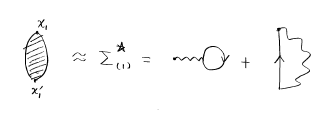
\includegraphics[width = 10cm]{2-6-1.png}\label{Fig2.6.1}
\end{center}


In this approximation, a particle moves in a single particle potential that is created by all the other particles by way of interaction potential. But, in this approximation, these internal fermion lines are just non-interacting Green's function, so that background particles which create an effective single-particle potential are treated as non-interacting. But, in reality, the background particles also move under the effective single-particle potential. Therefore, it is much more natural to replace these non-interacting Green's functions by the interacting Green's function itself. Namely,
\begin{center} 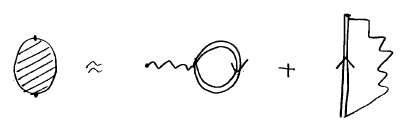
\includegraphics[width=8cm]{2-6-2.png} \label{Fig2.6.2}\end{center}
where these bold lines themselves are given by this proper selfenergy via Dyson equation,
\begin{center} 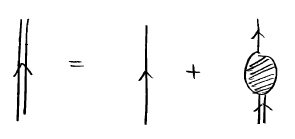
\includegraphics[width=6cm]{2-6-3.png}\label{Fig2.6.3} \end{center}
We will study these equations in details.

To this end, we will consider a spin$=\frac{1}{2}$ fermion system in a static spin-independent potential $U(\mathbf{x})$.
\[\begin{split}
\hat{H}_{0} &= \int \mathrm{d}^{3}x \  \psi_{\alpha}^{\dagger}(x)\left[ -\frac{\hbar^{2}\nabla^{2}}{2m} + U(\mathbf{x}) \right] \psi_{\alpha}(x) \\
\hat{H}_{1} &= \frac{1}{2} \int \mathrm{d}^{3}x \mathrm{d}^{3}x^{'} \ \psi_{\alpha}^{\dagger}(x) \psi_{\beta}^{\dagger}(x^{'})V(x-x^{'})\psi_{\beta}(x^{'})\psi_{\alpha}(x)
\end{split}\]
Here we assumed the spin-independent interaction potential for simplicity.

Within the self-consistent Hatree-Fock approximation, the Dyson equation is given by these two equations:
\[ \left \{ \begin{split}
G(x,y)&= G^{0}(x,y) + \int \mathrm{d}^{4}x_{1} \mathrm{d}^{4}x_{1}^{'} \ G^{0}(x,x_{1}) \Sigma^{\bigstar}% a star character
(x_{1},x_{1}^{'})G(x_{1}^{'},y)\\
\hbar \Sigma^{\bigstar}
(x_{1},x_{1}^{'})&= -i \delta(t_{1}-t_{1}^{'}) \times 
\left[ \delta(\mathbf{x}_{1}-\mathbf{x}_{1}^{'}) \ 2 \int \mathrm{d}^{3}x_{2} \left( \begin{split} &G(\mathbf{x}_{2},t_{2};\mathbf{x}_{2},t_{2}+0) V(\mathbf{x}_{1}-\mathbf{x}_{2}) 
\\- &G(\mathbf{x}_{1},t_{1};\mathbf{x}_{1}^{'},t_{1}+0) V(\mathbf{x}_{1}-\mathbf{x}_{1}^{'}) \end{split}\right)
\right]
\end{split}\right. \]
Where the factor $2$ comes from the spin summations.

Now, it is convenient to use a Fourier representation.
\[ \begin{split}
G(\mathbf{x},t;\mathbf{x}^{'},t^{'})&=\frac{1}{2\pi}\int \mathrm{d} \omega \mathrm{e}^{-i \omega (t-t^{'})} G(\mathbf{x},\mathbf{x}^{'};\omega)\\
G^{0}(\mathbf{x},t;\mathbf{x}^{'},t^{'})&=\frac{1}{2\pi}\int \mathrm{d} \omega \mathrm{e}^{-i \omega (t-t^{'})} G^{0}(\mathbf{x},\mathbf{x}^{'};\omega)\\
\Sigma^{\bigstar}(\mathbf{x},t;\mathbf{x}^{'},t^{'})&=
\delta(t-t^{'})\Sigma^{\bigstar}(\mathbf{x},\mathbf{x}^{'})\\
&=\frac{1}{2\pi}\int \mathrm{d} \omega \mathrm{e}^{-i \omega (t-t^{'})}\Sigma^{\bigstar}(\mathbf{x},\mathbf{x}^{'})
\end{split} \]
\begin{equation}
G(\mathbf{x},\mathbf{y};\omega)=G^{0}(\mathbf{x},\mathbf{y};\omega)+\int \mathrm{d}^{3}\mathbf{x}_{1} \mathrm{d}^{3}\mathbf{x}^{'}_{1} \ G^{0}(\mathbf{x},\mathbf{x}_{1};\omega) \times \Sigma^{\bigstar}(\mathbf{x}_{1},\mathbf{x}^{'}_{1})G(\mathbf{x}^{'}_{1},\mathbf{y},\omega)
\label{Eqs2.6.1}\end{equation}
\begin{equation}\begin{split}
\hbar\Sigma^{\bigstar}(\mathbf{x}_{1},\mathbf{x}^{'}_{1})
=&-i 2 \delta(\mathbf{x}_{1}-\mathbf{x}^{'}_{1}) \int \mathrm{d}^{3}\mathbf{x}_{2} \ V(\mathbf{x}_{1}-\mathbf{x}_{2}) \times \frac{1}{2\pi}\int \mathrm{d} \omega \mathrm{e}^{i \omega 0 t} G(\mathbf{x}_{2},\mathbf{x}_{2};\omega)\\
&+i V(\mathbf{x}_{1}-\mathbf{x}^{'}_{1}) \frac{1}{2\pi}\int \mathrm{d} \omega \mathrm{e}^{i \omega 0 t} G(\mathbf{x}_{1},\mathbf{x}_{1}^{'};\omega)
\end{split}\label{Eqs2.6.2}\end{equation}
Let us also introduce the orthonormal eigenfunctions of $H_{0}$.
\[ H_{0} \ \varphi_{j}^{0}(\mathbf{x}) \equiv \left[ -\frac{\hbar^{2}\nabla^{2}}{2m} + U(\mathbf{x}) \right]\varphi_{j}^{0}(\mathbf{x}) = \epsilon_{j}\varphi_{j}^{0}(\mathbf{x}) \]
In terms of  this eigenfunctions, the field operator in the interaction representation can be expanded as
\[ \left \{ \begin{split}
\psi(\mathbf{x},t) &= \sum_{j} \varphi_{j}(\mathbf{x})c_{j}\mathrm{e}^{-i\frac{\epsilon_{j}t}{\hbar}}\\
\psi^{\dagger}(\mathbf{x},t) &= \sum_{j} \varphi^{*}_{j}(\mathbf{x})c_{j}^{\dagger}\mathrm{e}^{+i\frac{\epsilon_{j}t}{\hbar}}
\end{split} \right. \]
where we used \[\mathrm{e}^{+i\frac{H_{0}t}{\hbar}}c_{j}\mathrm{e}^{-i\frac{H_{0}t}{\hbar}}=\mathrm{e}^{-i\frac{\epsilon_{j}t}{\hbar}}c_{j}\]
In terms of them, the non-interacting Green's function can be calculated as
\[ \begin{split}
i G^{0}(\mathbf{x},t;\mathbf{x}^{'},t^{'})=& \langle \Phi_{0} | \Gamma [ \psi_{I}(\mathbf{x},t) \psi_{I}^{\dagger}(\mathbf{x}^{'},t^{'}) ] | \Phi_{0} \rangle\\
=& \  \theta(t-t^{'}) \  \langle \Phi_{0} | \psi_{I}(\mathbf{x},t) \psi_{I}^{\dagger}(\mathbf{x}^{'},t^{'}) | \Phi_{0} \rangle \\
&-\theta(t^{'}-t) \  \langle \Phi_{0} | \psi_{I}^{\dagger}(\mathbf{x}^{'},t^{'}) \psi_{I}(\mathbf{x},t) | \Phi_{0} \rangle \\
=& \ \theta(t-t^{'}) \sum_{j} \varphi_{j}^{0}(\mathbf{x})\varphi_{j}^{0*}(\mathbf{x}^{'}) \mathrm{e}^{-i\frac{\epsilon_{j}}{\hbar}(t-t^{'})}
\times \langle \Phi_{0} | c_{j}c_{j}^{\dagger} | \Phi_{0} \rangle \\
&-\theta(t^{'}-t) \sum_{j} \varphi_{j}^{0}(\mathbf{x})\varphi_{j}^{0*}(\mathbf{x}^{'}) \mathrm{e}^{-i\frac{\epsilon_{j}}{\hbar}(t-t^{'})}
\times \langle \Phi_{0} | c_{j}^{\dagger}c_{j} | \Phi_{0} \rangle\\
=&\sum_{j} \varphi_{j}^{0}(\mathbf{x})\varphi_{j}^{0*}(\mathbf{x}^{'}) \mathrm{e}^{-i\frac{\epsilon_{j}}{\hbar}(t-t^{'})} \times \left \{ \theta(t-t^{'})\langle \Phi_{0} | c_{j}c_{j}^{\dagger} | \Phi_{0} \rangle
-\theta(t^{'}-t)\langle \Phi_{0} | c_{j}^{\dagger}c_{j} | \Phi_{0} \rangle \right \}\\
=& \sum_{j} \varphi_{j}^{0}(\mathbf{x})\varphi_{j}^{0*}(\mathbf{x}^{'}) \mathrm{e}^{-i\frac{\epsilon_{j}}{\hbar}(t-t^{'})} \times \left \{ \theta(t-t^{'})\theta(\epsilon_{j}^{0}-\epsilon_{F}^{0}) - \theta(t^{'}-t)\theta(-\epsilon_{j}^{0}+\epsilon_{F}^{0}) \right \}
\end{split} \]
where $\epsilon_{F}^{0}$ is the energy of the highest filled state.

The Fourier transformation leads to
\begin{equation}\label{Eqs2.6.3}
G^{0}(\mathbf{x},\mathbf{x}^{'};\omega) = \sum_{j} \varphi_{j}^{0}(\mathbf{x})\varphi_{j}^{0*}(\mathbf{x}^{'}) \times \left[
\frac{\theta(\epsilon_{j}^{0}-\epsilon_{F}^{0})}{\omega-\hbar^{-1}\epsilon_{j}^{0}+i\eta} +\frac{\theta(\epsilon_{F}^{0}-\epsilon_{j}^{0})}{\omega-\hbar^{-1}\epsilon_{j}^{0}-i\eta}
 \right]
\end{equation}
The particle density at $\mathbf{x}$ in the unperturbed ground state is estimated as
\[ \begin{split} n^{0}(\mathbf{x}) =& -i \  2 \ \frac{1}{2\pi} \int \mathrm{d} \omega \mathrm{e}^{i\omega 0 t} G^{0}(\mathbf{x},\mathbf{x};\omega)\\
=& 2 \sum_{j} |\varphi_{j}^{0}(\mathbf{x})|^{2} \theta(\epsilon_{F}^{0}-\epsilon_{j}^{0})
\end{split}\]
where the factor 2 comes from spin.

The total number of fermions is given by its spatial integral:
\[ N = \int \mathrm{d}^{3}\mathbf{x} n^{0}(\mathbf{x}) = 2 \sum_{j} \theta(\epsilon_{F}^{0}-\epsilon_{j}^{0}) \]
where we assume the normalization of $\varphi_{j}^{0}(\mathbf{x})$

These three equations(eq.(\ref{Eqs2.6.1}),eq.(\ref{Eqs2.6.2}),eq.(\ref{Eqs2.6.3})) comprise a set of coupled equations for the Green's function G.

To solve these coupled equations in favor for G, let us apply a following differential operator onto eq.(\ref{Eqs2.6.1})
\[ L_{1} = \hbar \omega + \frac{\hbar^{2}\nabla^{2}}{2m} - V(\mathbf{x})\]
If we apply this onto $G^{0}(\mathbf{x},\mathbf{y};\omega)$, we obtain the delta function in space,
\[\begin{split} L_{1} \ G^{0}(\mathbf{x},\mathbf{y};\omega) =& \sum_{j}(\hbar\omega - \epsilon_{j}^{0})\varphi_{j}^{0}(\mathbf{x})\varphi_{j}^{0*}(\mathbf{y})
 \times \left[
\frac{\theta(\epsilon_{j}^{0}-\epsilon_{F}^{0})}{\omega-\hbar^{-1}\epsilon_{j}^{0}+i\eta} +\frac{\theta(\epsilon_{F}^{0}-\epsilon_{j}^{0})}{\omega-\hbar^{-1}\epsilon_{j}^{0}-i\eta}
 \right]\\
=& \hbar \sum_{j} \varphi_{j}^{0}(\mathbf{x})\varphi_{j}^{0*}(\mathbf{y}) = \hbar \delta^{3}(\mathbf{x}-\mathbf{y})
\end{split} \]
Thus, an application of $L_{1}$ onto eq.(\ref{Eqs2.6.1}) leads to
\[ L_{1} \ G(\mathbf{x},\mathbf{y};\omega) = \hbar\delta^{3}(\mathbf{x}-\mathbf{y}) + \int \mathrm{d}^{3}\mathbf{x}_{1}^{'} 
\hbar\Sigma^{\bigstar}(\mathbf{x},\mathbf{x}_{1}^{'})G(\mathbf{x}_{1}^{'},\mathbf{y};\omega) \]
or equivalently
\begin{equation}\label{Eqs2.6.4}
\left[ \hbar\omega + \frac{\hbar^{2}\nabla^{2}_{\mathbf{x}}}{2m} - V(\mathbf{x}) \right] G(\mathbf{x},\mathbf{y};\omega) - \int \mathrm{d}^{3} \mathbf{x}^{'} \hbar \Sigma^{\bigstar}(\mathbf{x},\mathbf{x}^{'})G(\mathbf{x}^{'},\mathbf{y};\omega) = \hbar\delta^{3}(\mathbf{x}-\mathbf{y})
\end{equation}
Generally, such a linearized integral equation can be solved in terms of following set of eigenstates $\varphi_{j}(\mathbf{x})$
\begin{equation} \label{Eqs2.6.5}
 \left[ -\frac{\hbar^{2}\nabla^{2}_{\mathbf{x}}}{2m} + V(\mathbf{x}) \right]\varphi_{j}(\mathbf{x})+\int \mathrm{d}^{3} \mathbf{x}^{'} \hbar \Sigma^{\bigstar}(\mathbf{x},\mathbf{x}^{'})\varphi_{j}(\mathbf{x}^{'})=\epsilon_{j}\varphi_{j}(\mathbf{x}) \end{equation}

\[ \begin{split} iG_{\alpha\beta}(\mathbf{x},t;\mathbf{x}^{'},t^{'}) =
 \sum_{n} \{ &\theta(t-t^{'}) \mathrm{e}^{\frac{-i(E_{n}-E)(t-t^{'})}{\hbar}} \times \langle \Psi_{0} | \psi_{\alpha}(\mathbf{x}) | \Psi_{n} \rangle \langle \Psi_{n} | \psi_{\beta}^{\dagger}(\mathbf{x}^{'}) | \Psi_{0} \rangle  \\
- \ &\theta(t^{'}-t) \mathrm{e}^{\frac{-i(E_{n}-E)(t-t^{'})}{\hbar}} \times \langle \Psi_{0} | \psi_{\beta}^{\dagger}(\mathbf{x}^{'}) | \Psi_{n} \rangle \langle \Psi_{n} | \psi_{\alpha}(\mathbf{x}) | \Psi_{0} \rangle \}
\end{split} \]
\[ \begin{split} G_{\alpha\beta}(\mathbf{x},\mathbf{x}^{'};\omega) = \sum_{n} [ 
&\frac{\langle \Psi_{0} | \psi_{\alpha}(\mathbf{x}) | \Psi_{n} \rangle \langle \Psi_{n} | \psi_{\beta}^{\dagger}(\mathbf{x}^{'}) | \Psi_{0} \rangle}{\omega-\hbar^{-1}(E_{n}-E)+i\eta} \\
+&\frac{\langle \Psi_{0} | \psi_{\beta}^{\dagger}(\mathbf{x}^{'}) | \Psi_{n} \rangle \langle \Psi_{n} | \psi_{\alpha}(\mathbf{x}) | \Psi_{0} \rangle}{\omega-\hbar^{-1}(E_{n}-E)-i\eta} ]
\end{split} \]
\[ \frac{1}{2\pi} \int_{-\infty}^{+\infty} \mathrm{d}\omega G_{\alpha\beta}(\mathbf{x},\mathbf{x}^{'};\omega)\mathrm{e}^{i\omega 0 t} = i \sum_{n} \langle \Psi_{0} | \psi_{\beta}^{\dagger}(\mathbf{x}^{'}) | \Psi_{n} \rangle \langle \Psi_{n} | \psi_{\alpha}(\mathbf{x}) | \Psi_{0} \rangle \]
\[ {\left ( i \int_{-\infty}^{+\infty} \mathrm{d} \omega G(\mathbf{x},\mathbf{x}^{'};\omega)\mathrm{e}^{i \omega 0 t} \right )}^{*} = i \int_{-\infty}^{+\infty} \mathrm{d} \omega G(\mathbf{x}^{'},\mathbf{x};\omega)\mathrm{e}^{i \omega 0 t} \]
where $\hbar\Sigma^\bigstar$ play role of a static but no-local potential.

Since $\Sigma^\bigstar$ is hermitian,\[\Sigma^{\bigstar*}(\mathbf{x},\mathbf{x}^{'}) = \Sigma^\bigstar(\mathbf{x}^{'},\mathbf{x}) \]
$\{\varphi_{j}\}$ comprises complete set of orthonormal eigenfunctions with
\[ \sum_{j} \varphi_{j}(\mathbf{x})\varphi_{j}^{*}(\mathbf{x}^{'}) = \delta^{3}(\mathbf{x}-\mathbf{x}^{'}) \]
\[ \int \mathrm{d}^3 \mathbf{x} \varphi_j^*(\mathbf{x})\varphi_m(\mathbf{x}) = \delta_{jm} \]
and $\epsilon_j$ is real.

In terms of this eigenstates, the Green's function satisfying eq.(\ref{Eqs2.6.4}) is roughly given in a following form:
\[ G(\mathbf{x},\mathbf{y};\omega) \sim \sum_j \varphi_j(\mathbf{x})\varphi_j^*(\mathbf{y}) \cdot \frac{1}{\omega-\hbar^{-1}\epsilon_j} \]


According to eq.(\ref{2.3.2}), the particle density and total number of the particles are given by the frequency integral of this Green's function.
\[ n(\mathbf{x}) = - i \ 2 \cdot \frac{1}{2\pi} \int_{-\infty}^{+\infty} \mathrm{d} \omega \mathrm{e}^{i \omega  0 t} G(\mathbf{x},\mathbf{x};\omega) \]
\[ N = -i \ 2 \cdot \frac{1}{2\pi} \int \mathrm{d}^3 \mathbf{x} \int_{-\infty}^{+\infty} \mathrm{d} \omega \mathrm{e}^{i \omega  0 t} G(\mathbf{x},\mathbf{x};\omega) \]


But, since the perturbation $\hat{H}_1$ conserves the total number of particles, the number of particles thus calculated should be equal to the number of particles in the unperturbed ground state. To make it possible, the denominator in the r.h.s. of this equation should acquire an infinitesimally small imaginary part like this:
\begin{equation}\label{Eqs2.6.6}
G(\mathbf{x},\mathbf{y};\omega) = \sum_j \varphi_j(\mathbf{x}) \varphi_j^* (\mathbf{y})
\left[ \frac{\theta(\epsilon_j - \epsilon_F)}{\omega - \hbar^{-1}\epsilon_j + i \eta} + \frac{\theta(\epsilon_F - \epsilon_j)}{\omega - \hbar^{-1}\epsilon_j - i \eta} \right]   \quad (\eta > 0)
\end{equation}
$\epsilon_F $ here denote the energy of the highest filled state of these orthonormal eigenstates, which satisfies
\[ \sum_j \theta(\epsilon_F - \epsilon_j) = N \equiv \sum_j \theta(\epsilon_F^0 - \epsilon_j^0) \]
substituting this solution back into eq.(\ref{Eqs2.6.2}), we obtain the self-energy itself, which is given by these orthonormal eigenstates.
\begin{equation}\label{Eqs2.6.7} \begin{split}
 \hbar \Sigma^\bigstar (\mathbf{x}_1,\mathbf{x}_1^{'}) =
& 2 \ \delta(\mathbf{x}_1 - \mathbf{x}_1^{'}) \int \mathrm{d}^3 \mathbf{x}_2 V(\mathbf{x}_1 - \mathbf{x}_2) \times \sum_j |\varphi_j(\mathbf{x}_2)|^2 \theta(\epsilon_F - \epsilon_j) \\
&- V(\mathbf{x}_1 - \mathbf{x}_1^{'}) \sum_j \varphi_j (\mathbf{x}_1) \varphi_j^* (\mathbf{x}_1^{'}) \theta(\epsilon_F - \epsilon_j) \\
=& \delta(\mathbf{x}_1 - \mathbf{x}_1^{'}) \int \mathrm{d}^3 \mathbf{x}_2 V(\mathbf{x}_1 - \mathbf{x}_2) n(\mathbf{x}_2) \quad \text{(Fock term)}\\
&- V(\mathbf{x}_1 - \mathbf{x}_1^{'})\sum_j \varphi_j(\mathbf{x}_1)\varphi_j^*(\mathbf{x}_1^{'})\theta(\epsilon_F - \epsilon_j) \quad \text{(Hartree term)}
\end{split}\end{equation}
Within this HF approximation, the self-energy consists of two terms. One is a local term propotional to particle density, and the other is non-local exchange term. These two are often called as Hartree term and Fock term respectively.

To summarize, eq.(\ref{Eqs2.6.5}) and eq.(\ref{Eqs2.6.7}) comprise a self-consistent equations for the orthonormal eigenstates $\varphi_j$ and its eigenvalue $\epsilon_j$.

Namely, once  $\varphi_j$ and $\epsilon_j$ are given, the self-energy $\Sigma^\bigstar$ are calculated by eq.(\ref{Eqs2.6.7}). In terms of this self-energy, the orthonormal eigenstates $\varphi_j$ and $\epsilon_j$ are recalculated. This process is repeated, until a self-consistent solution for \{$\varphi_j$\} and \{$\epsilon_j$\} is obtained.

Once the self-consistent solution is obtained, we can calculate Green's function from eq.(\ref{Eqs2.6.6}), from which we can calculate various physical quantities such as ground state energy and ground state expectation value of single particle operators.
\begin{center}-------------------\end{center}

This is all about the Hartree-Fock approximation, which is quite commonly used in condensed matter physics research.

In the following two sections, I will describe two other standard approximation scheme commonly used in the contemporary research.

\section{Imperfect Fermi Gas}%wsz 2-7
The first system considered is a dilute Fermi gas with strong short-range repulsive interaction, which is somtimes called as ``imperfect Fermi gas".

We assume that the repulsive interaction is s-wave like, so that the potential depends only on a spatial distance between two particles.

To be specific, we assume that the repulsive interaction is described by a square-well shape potential.
\begin{center} \label{Fig2.7.1} 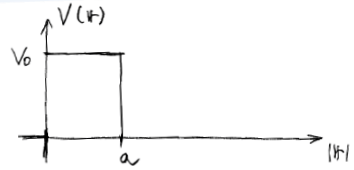
\includegraphics[width=6cm]{2-7-1.png}
\end{center}
where positive $V_0$ means repulsive and ``$a$" represents an interaction range.

``strong short-range repulsive interaction" means that ``$V_0$" will be taken to be sufficiently large, but ``$a$" will be taken to be small.
\[ \left \{ \begin{split} V_0 &\rightarrow \text{large} \\ a &\rightarrow \text{small} \end{split} \right. \]

For the kinetic energy part, we simply assume the free electron Hamiltonian
\[H_0 = \sum_\alpha \int \mathrm{d}^3 \mathbf{x} \psi_\alpha^\dagger (\mathbf{x}) \left[-\frac{\hbar^2\nabla^2_{\mathbf{x}}}{2m}\right]\psi_\alpha(\mathbf{x})\]
whose dispersion take a parabolic form.
\begin{center} \label{Fig2.7.2} 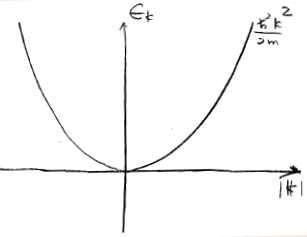
\includegraphics[width=3cm]{2-7-2.png} \end{center}

``dilute Fermi gas" means that the chemical potential is chosen so that the Fermi momentum is sufficiently small. $$k_F \rightarrow \text{small}$$

Now $k_F a$ comprises a dimensionless quantity. The natural coupling constant for ``imperfect Fermi gas" is ``$k_F a$". Namely, we are going to analyize the ``imperfect Fermi gas" by treating ``$k_F a$" as a small parameter. Thereby, physical quantities such as ground state energy, chemical potential and quasi-particle spectrum are calculated, perturbatively in small $k_F a$.
\[ \text{e.g.)} \quad \frac{E}{N} = \frac{\hbar^2 k_F^2}{2m} \left[ A + B(k_F a) + C{(k_F a)}^2 + \ldots \right] \]

To do this perturbation expansion, systematically, let us begin with the 2nd order contribution to the proper self energy.

According to eq.(\ref{Eqs2.6.4}), the 2nd order contribution can be enumerated as follows:
\begin{center}\label{Fig2.7.3} 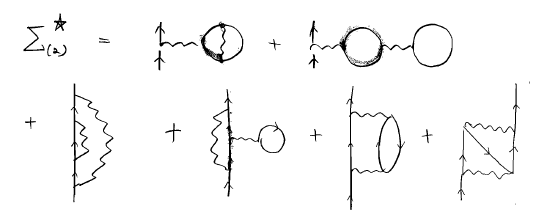
\includegraphics[width=8cm]{2-7-3.png} \end{center}

For the uniform electron gas case, these four term exactly reduce to zero.
\begin{center}-----------------------------\end{center}

\begin{wrapfigure}{l}{3.5cm}
\label{Fig2.7.4} 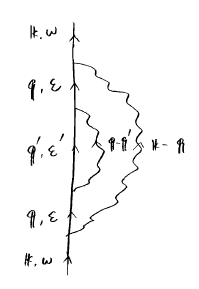
\includegraphics[width=3cm]{2-7-4.png}
\end{wrapfigure}
For example, consider this diagram.

The self energy part can be calculated as this.
\[ \begin{split} & {\left(\frac{i}{\hbar} \right)}^2 \frac{1}{\left( 2\pi \right)^8} \int \mathrm{d}^3 \mathbf{q} \int \mathrm{d}\epsilon \int \mathrm{d}^3 \mathbf{q}^{'} \int \mathrm{d} \epsilon^{'} \\
& \  \times \left\{ V(\mathbf{q}-\mathbf{q}^{'})V(\mathbf{k}-\mathbf{q})\mathrm{e}^{i \epsilon^{'} 0 t} G_0(\mathbf{q}^{'},\epsilon^{'}) \times \left[ G_0(\mathbf{q},\epsilon) \right]^2 \right \} \end{split} \]

where
\[ G_0(\mathbf{q},\epsilon) \equiv \frac{\theta(|\mathbf{q}|-k_F)}{\epsilon - \epsilon_{\mathbf{q}}+i \eta} + \frac{\theta(k_F-|\mathbf{q}|)}{\epsilon - \epsilon_{\mathbf{q}}-i \eta} \]

Putting this into here, this part becomes like this:
\[ \int \frac{\mathrm{d}\epsilon^{'}}{2\pi} \left[ \frac{\theta(|\mathbf{q}|-k_F)}{\epsilon^{'} - \epsilon_{\mathbf{q}^{'}}+i \eta} + \frac{\theta(k_F-|\mathbf{q}|)}{\epsilon^{'} - \epsilon_{\mathbf{q}^{'}}-i \eta} \right]^2 \]

Since $$\theta(|\mathbf{q}|-k_F)\theta(k_F-|\mathbf{q}|) = 0$$

 the cross term vanishes, so that we have
\[ \int \frac{\mathrm{d}\epsilon^{'}}{2\pi} \left[ \frac{\theta(|\mathbf{q}|-k_F)}{\left(\epsilon^{'} - \epsilon_{\mathbf{q}^{'}}+i \eta\right)^2} + \frac{\theta(k_F-|\mathbf{q}|)}{\left(\epsilon^{'} - \epsilon_{\mathbf{q}^{'}}-i \eta\right)^2} \right] \]

Now we can integrate this, by closing the contour either in the upper half plane or in the lower half plane(By using the method of contour integration).

But, since both of these two are the second order pole, the contour integration always reduce to zero, irrespective of whether the integration is carried out in the upper--half plane or in the lower--half plane.

Therefore, this contribution always reduce to zero. Similarly, we can immediately see that all of these also reduce to zero, because these parts give the same integration as this.

\begin{wrapfigure}[8]{l}{4.5cm}
\label{Fig2.7.5} 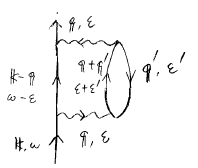
\includegraphics[width=4cm]{2-7-5.png}
\end{wrapfigure}
Thus, we have only to calculate these two contributions,
\[ \begin{split} &- \left( \frac{i}{\hbar}\right)^2 \frac{1}{\left( 2\pi \right)^8} \int \mathrm{d}^3 \mathbf{q} \int \mathrm{d}\epsilon \int \mathrm{d}^3 \mathbf{q}^{'} \int \mathrm{d} \epsilon^{'} \\
&\times \left\{ \ V^2(\mathbf{q})G_0(\mathbf{k}-\mathbf{q},\omega-\epsilon) \times G_0(\mathbf{q} + \mathbf{q}^{'}, \epsilon + \epsilon^{'}) G_0(\mathbf{q}^{'},\mathbf{\epsilon}^{'}) \right\} \end{split} \]

%Let me try this first.

Let me first integrate over these internal frequencies by using the method of contour integration.
\[ \begin{split} \int \frac{\mathrm{d}\epsilon}{2\pi} \int \frac{\mathrm{d}\epsilon^{'}}{2\pi}
&\left[ \frac{\theta(|\mathbf{k}-\mathbf{q}|-k_F)}{\omega - \epsilon - \epsilon_{\mathbf{k}-\mathbf{q}}+i \eta} + \frac{\theta(k_F-|\mathbf{k}-\mathbf{q}|)}{\omega - \epsilon - \epsilon_{\mathbf{k}-\mathbf{q}}-i \eta} \right] \\
& \times \left[ \frac{\theta(|\mathbf{q}+\mathbf{q}^{'}|-k_F)}{\epsilon + \epsilon^{'} - \epsilon_{\mathbf{q}+\mathbf{q}^{'}}+i \eta} + \frac{ \theta(k_F-|\mathbf{q}+\mathbf{q}^{'}|)}{\epsilon + \epsilon^{'} - \epsilon_{\mathbf{q}+\mathbf{q}^{'}}-i \eta} \right] \\
& \times \left[ \frac{\theta(|\mathbf{q}^{'}|-k_F)}{\epsilon^{'} - \epsilon_{\mathbf{q}^{'}}+i \eta} + \frac{\theta(k_F-|\mathbf{q}^{'}|)}{\epsilon^{'} - \epsilon_{\mathbf{q}^{'}}-i \eta} \right]
\end{split} \]
I will first integrate over $\epsilon$, whose integrand is the product between these two:
\[\left[ \frac{\theta(|\mathbf{k}-\mathbf{q}|-k_F)}{\omega - \epsilon - \epsilon_{\mathbf{k}-\mathbf{q}}+i \eta} + \frac{\theta(k_F-|\mathbf{k}-\mathbf{q}|)}{\omega - \epsilon - \epsilon_{\mathbf{k}-\mathbf{q}}-i \eta} \right]
\times \left[ \frac{\theta(|\mathbf{q}+\mathbf{q}^{'}|-k_F)}{\epsilon + \epsilon^{'} - \epsilon_{\mathbf{q}+\mathbf{q}^{'}}+i \eta} + \frac{ \theta(k_F-|\mathbf{q}+\mathbf{q}^{'}|)}{\epsilon + \epsilon^{'} - \epsilon_{\mathbf{q}+\mathbf{q}^{'}}-i \eta} \right] \]

From this product, we have four terms.

But these two reduce to zero, when the contour integration over $\epsilon$ is carried out.
\[ \frac{\ldots}{\omega - \epsilon - \epsilon_{\mathbf{k}-\mathbf{q}} \pm i \eta} \cdot \frac{ \ldots}{\epsilon + \epsilon^{'} - \epsilon_{\mathbf{q}+\mathbf{q}^{'}} \mp i \eta} \]

Namely these two have a pole in the upper half plane, while these two have a pole in the lower half plane. Thus, for this term, we can close the contour in the lower half plane, while for this term, we can close the contour in the upper half plane, which reduce them to zero under the integration.

On the one hand, these combinations always have a pole both in the upper half plane and in the lower half plane.
\[ \frac{\ldots}{\omega - \epsilon - \epsilon_{\mathbf{k}-\mathbf{q}} \pm i \eta} \cdot \frac{ \ldots}{\epsilon + \epsilon^{'} - \epsilon_{\mathbf{q}+\mathbf{q}^{'}} \pm i \eta} \]

Thus, irrespective of how the contour is closed, these two combinations give finite contribution.
\[\begin{split} \int \frac{\mathrm{d} \epsilon}{2\pi}
&\left \{ \frac{\theta(|\mathbf{k}-\mathbf{q}|-k_F)}{\omega - \epsilon - \epsilon_{\mathbf{k}-\mathbf{q}} + i \eta} \cdot \frac{ \theta(|\mathbf{q}+\mathbf{q}^{'}|-k_F)}{\epsilon + \epsilon^{'} - \epsilon_{\mathbf{q}+\mathbf{q}^{'}} + i \eta}
+ \frac{\theta(k_F-|\mathbf{k}-\mathbf{q}|)}{\omega - \epsilon - \epsilon_{\mathbf{k}-\mathbf{q}} - i \eta} \cdot \frac{ \theta(k_F-|\mathbf{q}+\mathbf{q}^{'}|)}{\epsilon + \epsilon^{'} - \epsilon_{\mathbf{q}+\mathbf{q}^{'}} - i \eta} \right \}\\
& = -i \cdot \frac{\theta(|\mathbf{k}-\mathbf{q}|-k_F)\theta(|\mathbf{q}+\mathbf{q}^{'}|-k_F)}{\omega - \epsilon_{\mathbf{k}-\mathbf{q}} + \epsilon^{'} - \epsilon_{\mathbf{q}+\mathbf{q}^{'}} + 2 i \eta }
+i \cdot \frac{\theta(k_F-|\mathbf{k}-\mathbf{q}|)\theta(k_F-|\mathbf{q}+\mathbf{q}^{'}|)}{\omega - \epsilon_{\mathbf{k}-\mathbf{q}} + \epsilon^{'} - \epsilon_{\mathbf{q}+\mathbf{q}^{'}} - 2 i \eta }
\end{split} \]

Let me next integrate over $\epsilon^{'}$, by subtituting this into here. From this product, we again have four terms.

Now these two have a pole in the upper half plane, while these two have a pole in the lower half plane. Due to the same reason, only these two combinations give us a finite contribution.
\[\begin{split}  (-i) \{
&\int \frac{\mathrm{d}\epsilon^{'}}{2\pi} \  \frac{\theta(|\mathbf{k}-\mathbf{q}|-k_F)\theta(|\mathbf{q}+\mathbf{q}^{'}|-k_F)}{\epsilon^{'} + \omega - \epsilon_{\mathbf{k}-\mathbf{q}} - \epsilon_{\mathbf{q}+\mathbf{q}^{'}} + 2 i \eta }
\cdot \frac{\theta(k_F-|\mathbf{q}^{'}|)}{\epsilon^{'}-\epsilon_{\mathbf{q}^{'}}-i \eta} \\
&- \int \frac{\mathrm{d}\epsilon^{'}}{2\pi} \ \frac{\theta(k_F-|\mathbf{k}-\mathbf{q}|)\theta(k_F-|\mathbf{q}+\mathbf{q}^{'}|)}{\epsilon^{'} + \omega - \epsilon_{\mathbf{k}-\mathbf{q}} - \epsilon_{\mathbf{q}+\mathbf{q}^{'}} - 2 i \eta }
\cdot \frac{\theta(|\mathbf{q}^{'}|-k_F)}{\epsilon^{'}-\epsilon_{\mathbf{q}^{'}}+i \eta} \} \\
=(-i) \{
&i \frac{\theta(|\mathbf{k}-\mathbf{q}|-k_F)\theta(|\mathbf{q}+\mathbf{q}^{'}|-k_F)\theta(k_F-|\mathbf{q}^{'}|)}{\omega - \epsilon_{\mathbf{k}-\mathbf{q}}-\epsilon_{\mathbf{q}+\mathbf{q}^{'}}+\epsilon_{\mathbf{q}^{'}}+3i \eta}\\
&+i \frac{\theta(k_F-|\mathbf{k}-\mathbf{q}|)\theta(k_F-|\mathbf{q}+\mathbf{q}^{'}|)\theta(|\mathbf{q}^{'}|-k_F)}{\omega - \epsilon_{\mathbf{k}-\mathbf{q}}-\epsilon_{\mathbf{q}+\mathbf{q}^{'}}+\epsilon_{\mathbf{q}^{'}}-3i \eta}
\}
 \end{split}\]

\begin{wrapfigure}[4]{l}{3.5cm}
\label{Fig2.7.6} 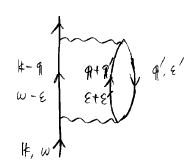
\includegraphics[width=3cm]{2-7-6.png}
\end{wrapfigure}

By substituting this into the original expression we obtain this:
\begin{equation} \label{Eqs2.7.1} \begin{split}
= & \frac{1}{\hbar^2} \int \frac{\mathrm{d}\mathbf{q}}{\left( 2\pi \right)^3} \int \frac{\mathrm{d}\mathbf{q}^{'}}{\left( 2\pi \right)^3} \\
& \times V^2(\mathbf{q}) \{
\frac{\theta(|\mathbf{k}-\mathbf{q}|-k_F)\theta(|\mathbf{q}+\mathbf{q}^{'}|-k_F)\theta(k_F-|\mathbf{q}^{'}|)}{\omega - \epsilon_{\mathbf{k}-\mathbf{q}}-\epsilon_{\mathbf{q}+\mathbf{q}^{'}}+\epsilon_{\mathbf{q}^{'}}}
\\
&+\frac{\theta(k_F-|\mathbf{k}-\mathbf{q}|)\theta(k_F-|\mathbf{q}+\mathbf{q}^{'}|)\theta(|\mathbf{q}^{'}|-k_F)}{\omega - \epsilon_{\mathbf{k}-\mathbf{q}}-\epsilon_{\mathbf{q}+\mathbf{q}^{'}}+\epsilon_{\mathbf{q}^{'}}}
\} \end{split}\end{equation}

\begin{wrapfigure}[4]{l}{3.5cm}
\label{Fig2.7.7} 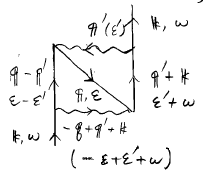
\includegraphics[width=3cm]{2-7-7.png}
\end{wrapfigure}
Similarly we can calculate the other 2nd order contribution to the proper self-energy.
\[ \begin{split} & \left(\frac{i}{\hbar}\right)^2 \frac{1}{(2\pi)^8} \int \mathrm{d}^3 \mathbf{q} \int \mathrm{d} \epsilon \int \mathrm{d}^3 \mathbf{q}^{'} \int \mathrm{d} \epsilon^{'}  \\
& \times \left\{ V(\mathbf{q}^{'})V(-\mathbf{q} + \mathbf{q}^{'}+\mathbf{k})
\times G_0(\mathbf{q}-\mathbf{q}^{'},\epsilon-\epsilon^{'})G_0(\mathbf{q},\epsilon)G_0(\mathbf{q}^{'}+\mathbf{k},\epsilon^{'}+\omega) \right\} \end{split}\]
\begin{center}---------------------------------------------\end{center}
\[ \begin{split}
&\quad \begin{split} \int \frac{\mathrm{d}\epsilon}{2\pi}\int \frac{\mathrm{d}\epsilon^{'}}{2\pi}
& \left[ \frac{\theta(|\mathbf{q}-\mathbf{q}^{'}|-k_F)}{\epsilon - \epsilon^{'}-\epsilon_{\mathbf{q}-\mathbf{q}^{'}}+i\eta} + \frac{\theta(k_F-|\mathbf{q}-\mathbf{q}^{'}|)}{\epsilon - \epsilon^{'}-\epsilon_{\mathbf{q}-\mathbf{q}^{'}}-i\eta} \right] \\
& \times \left[ \frac{\theta(|\mathbf{q}|-k_F)}{\epsilon -\epsilon_{\mathbf{q}}+i\eta} + \frac{\theta(k_F-|\mathbf{q}|)}{\epsilon -\epsilon_{\mathbf{q}}-i\eta} \right] \\
& \times \left[ \frac{\theta(|\mathbf{q}^{'}+\mathbf{k}|-k_F)}{\epsilon^{'}+\omega -\epsilon_{\mathbf{q}^{'}+\mathbf{k}}+i\eta} + \frac{\theta(k_F-|\mathbf{q}^{'}+\mathbf{k}|)}{\epsilon^{'}+\omega -\epsilon_{\mathbf{q}^{'}+\mathbf{k}}-i\eta} \right]
\end{split}
\\
& \begin{split}=
\int \frac{\mathrm{d}\epsilon}{2\pi} \{ & \frac{\theta(|\mathbf{q}|-k_F)}{\epsilon -\epsilon_{\mathbf{q}}+i\eta} + \frac{\theta(k_F-|\mathbf{q}|)}{\epsilon -\epsilon_{\mathbf{q}}-i\eta} \} \\
\times(-i)\{ & \frac{\theta(|\mathbf{q}-\mathbf{q}^{'}|-k_F)\theta(|\mathbf{q}^{'}+\mathbf{k}|-k_F)}{\epsilon + \omega - \epsilon_{\mathbf{q}^{'}+\mathbf{k}} - \epsilon_{\mathbf{q}-\mathbf{q}^{'}} + 2 i \eta }\\
&+\frac{\theta(k_F-|\mathbf{q}-\mathbf{q}^{'}|)\theta(k_F-|\mathbf{q}^{'}+\mathbf{k}|)}{\epsilon + \omega - \epsilon_{\mathbf{q}^{'}+\mathbf{k}} - \epsilon_{\mathbf{q}-\mathbf{q}^{'}} - 2 i \eta }
\}
\end{split}\\
& \begin{split}=  \ - \{&
\frac{\theta(|\mathbf{q}|-k_F)\theta(k_F-|\mathbf{q}-\mathbf{q}^{'}|)\theta(k_F-|\mathbf{q}^{'}+\mathbf{k}|)}{\omega+\epsilon_{\mathbf{q}} - \epsilon_{\mathbf{q}^{'}+\mathbf{k}}-\epsilon_{\mathbf{q}-\mathbf{q}^{'}}-3i \eta}\\
&+\frac{\theta(k_F-|\mathbf{q}|)\theta(|\mathbf{q}-\mathbf{q}^{'}|-k_F)\theta(|\mathbf{q}^{'}+\mathbf{k}|-k_F)}{\omega+\epsilon_{\mathbf{q}} - \epsilon_{\mathbf{q}^{'}+\mathbf{k}}-\epsilon_{\mathbf{q}-\mathbf{q}^{'}}+3i \eta} \} \end{split}
\end{split} \]

%\begin{wrapfigure}{l}{3.5cm}
%\label{Fig2.7.8} 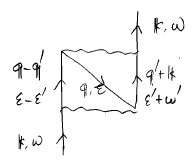
\includegraphics[width=3cm]{2-7-8.png}
%\end{wrapfigure}
\begin{center}---------------------------------------------\end{center}
\begin{equation} \label{Eqs2.7.2} \begin{split}
\rightarrow + \int \frac{\mathrm{d}^3 \mathbf{q}}{(2\pi)^3}\int \frac{\mathrm{d}^3 \mathbf{q}^{'}}{(2\pi)^3} \times [ &\frac{\theta(k_F-|\mathbf{q}|)\theta(|\mathbf{q}-\mathbf{q}^{'}|-k_F)\theta(|\mathbf{q}^{'}+\mathbf{k}|-k_F)}{\omega+\epsilon_{\mathbf{q}} - \epsilon_{\mathbf{q}^{'}+\mathbf{k}}-\epsilon_{\mathbf{q}-\mathbf{q}^{'}}} \\
& \ + \frac{\theta(|\mathbf{q}|-k_F)\theta(k_F-|\mathbf{q}-\mathbf{q}^{'}|)\theta(k_F-|\mathbf{q}^{'}+\mathbf{k}|)}{\omega+\epsilon_{\mathbf{q}} - \epsilon_{\mathbf{q}^{'}+\mathbf{k}}-\epsilon_{\mathbf{q}-\mathbf{q}^{'}}} ]
\end{split} \end{equation}

\begin{center}---------------------\end{center}

Observing these two expressions, notice that the integrants always contain the step function
\[ \theta(x) = \begin{cases} 1 & x > 0\\ 0 & x < 0 \end{cases} \]

which is nothing but the fermion distribution function at the zero temperature. Thus, this step function represents whether the intermediate state is particle-like excited state or hole-like excited state.

Due to this fermi distribution function, the momentum integral regions associated with these internal lines are highly restricted in the low density limit.

For example, this step function $\theta(k_F - |\mathbf{q}|)$ restrict this momentum ($\mathbf{q}$) integral within a small sphere whose radius is $k_F$. While these two step function $\theta(k_F-|\mathbf{q}-\mathbf{q}^{'}|)\theta(k_F-|\mathbf{q}^{'}+\mathbf{k}|)$ restrict these two momentum ($\mathbf{q}$ and $\mathbf{q}^{'}$) variables within a sphere of radius $k_F$.%

Accordingly, in the low density limit, the first term vanishes on the order of $k_F$, while the 2nd term vanishes on the order of $k_F^2$. Thus, we can regard that the first term dominates over the 2nd term, and these two contribution gives a quantity of the order of $k_F a$ in the low--density limit.

When generalizing this argument into higher order contribution to the proper self energy, we see that the leading order contribution in the low density limit comes only from the so--called ladder--type diagrams depicted here:

\begin{center}
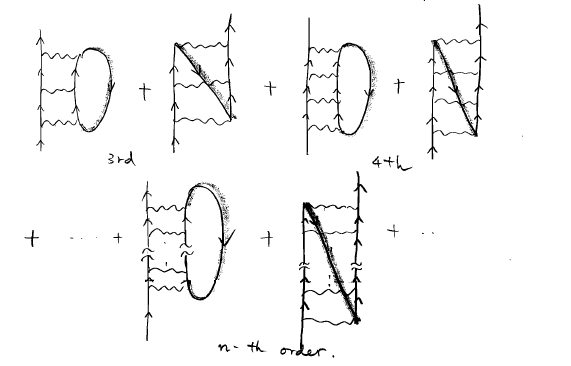
\includegraphics[width=8cm]{2-7-9.png}\label{Fig2.7.9}
\begin{equation} \label{Eqs2.7.3}\end{equation}
\end{center}

A basic feature of these ladder--type diagrams is as follows.

When all the interaction lines are put along the horizontal direction, any ladder--type diagrams contain \underline{only one} internal line which runs in the reverse direction to the other internal lines.

In these diagrams, \underline{these} are the ones which run in the reverse direction.

\begin{wrapfigure}[6]{l}{3.5cm}
\label{Fig2.7.10} 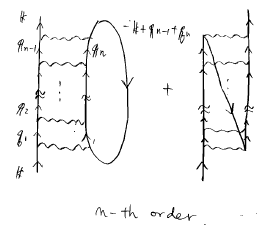
\includegraphics[width=3cm]{2-7-10.png}
\end{wrapfigure}
Due to this feature, the integrant of these diagram contains $(2n-1)$--numbers of fermi distribution function for particle times one fermi distribution function for hole.
\[ \begin{split}
= &\int \frac{\mathrm{d}^3 \mathbf{q}_1}{(2\pi)^3} \int \frac{\mathrm{d}^3 \mathbf{q}_2}{(2\pi)^3} \ldots \int \frac{\mathrm{d}^3 \mathbf{q}_n}{(2\pi)^3} V^n \\
& \times \{  \frac{
\begin{matrix} (2n-1)\text{number for particle lines} \\ \overbrace{ \theta(|\mathbf{q}_1|-k_F)\theta(|\mathbf{q}_2|-k_F)\ldots\theta(|\mathbf{q}_n|-k_F) } \end{matrix}
\begin{matrix} (1) \text{hole line} \\ \overbrace{ \theta(k_F-|-\mathbf{k}+\mathbf{q}_{n-1}+\mathbf{q}_n|)} \end{matrix}}{\text{(energy denominator)}}\\
& + o((k_F a)^2) \}
\end{split} \]

Any Feynman diagrams other than these ladder--type diagram contain at least two internal lines which run in the reverse direction to the other internal lines. Therefore, their leading order term always contain at least two hole lines, so that they are at most the 2nd order of $k_F a$.

For example, consider a following 3rd order perturbation to the proper self energy term.
\begin{center}
\label{Fig2.7.11} 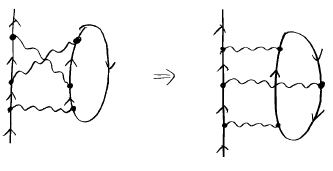
\includegraphics[width=6cm]{2-7-11.png}
\end{center}

When all the interaction lines are put in the horizontal way, this Feynman diagram contain two internal lines which run in the reverse direction to the other.
\begin{center}
\label{Fig2.7.12} 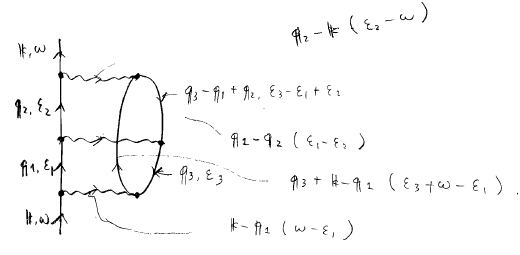
\includegraphics[width=6cm]{2-7-12.png}
\end{center}

\[ \begin{split}
-&\left(\frac{i}{\hbar}\right)^3 \ \frac{1}{(2\pi)^{12}} \int \mathrm{d}^3 \mathbf{q}_1 \int \mathrm{d} \epsilon_1 \int \mathrm{d}^3 \mathbf{q}_2 \int \mathrm{d} \epsilon_2 \int \mathrm{d}^3 \mathbf{q}_3 \int \mathrm{d} \epsilon_3 \\
&\times V(\mathbf{k}-\mathbf{q}_1)V(\mathbf{q}_1-\mathbf{q}_2)V(\mathbf{q}_2-\mathbf{k})\\
&\times G_0(\mathbf{q}_1,\epsilon_1)G_0(\mathbf{q}_2,\epsilon_2)G_0(\mathbf{q}_3,\epsilon_3)\\
&\times G_0(\mathbf{q}_3-\mathbf{q}_1+\mathbf{q}_2,\epsilon_3-\epsilon_1+\epsilon_2)G_0(\mathbf{q}_3-\mathbf{q}_1+\mathbf{k},\epsilon_3-\epsilon_1+\omega)
\end{split} \]
\begin{center}---------------------------------------------\end{center}
\[ \begin{split} &\int \frac{\mathrm{d}\epsilon_1}{2\pi} \int \frac{\mathrm{d}\epsilon_2}{2\pi} \int \frac{\mathrm{d}\epsilon_3}{2\pi}\left[ \frac{\theta(|\mathbf{q}_1|-k_F)}{\epsilon_1-\epsilon_{\mathbf{q}_1}+i \eta} + \frac{\theta(k_F-|\mathbf{q}_1|)}{\epsilon_1-\epsilon_{\mathbf{q}_1}-i \eta} \right] \\
& \times \left[ \frac{\theta(|\mathbf{q}_2|-k_F)}{\epsilon_2-\epsilon_{\mathbf{q}_2}+i \eta} + \frac{\theta(k_F-|\mathbf{q}_2|)}{\epsilon_2-\epsilon_{\mathbf{q}_2}-i \eta} \right] \times \left[ \frac{\theta(|\mathbf{q}_3|-k_F)}{\epsilon_3-\epsilon_{\mathbf{q}_3}+i \eta} + \frac{\theta(k_F-|\mathbf{q}_3|)}{\epsilon_3-\epsilon_{\mathbf{q}_3}-i \eta} \right] \\
& \times \left[ \frac{\theta(|\mathbf{q}_3-\mathbf{q}_1+\mathbf{q}_2|-k_F)}{\epsilon_3-\epsilon_1+\epsilon_2-\epsilon_{\mathbf{q}_3-\mathbf{q}_1+\mathbf{q}_2}+i \eta} + \frac{\theta(k_F-|\mathbf{q}_3-\mathbf{q}_1+\mathbf{q}_2|)}{\epsilon_3-\epsilon_1+\epsilon_2-\epsilon_{\mathbf{q}_3-\mathbf{q}_1+\mathbf{q}_2}-i \eta} \right]\\
& \times \left[ \frac{\theta(|\mathbf{q}_3-\mathbf{q}_1+\mathbf{k}|-k_F)}{\epsilon_3-\epsilon_1+\omega-\epsilon_{\mathbf{q}_3-\mathbf{q}_1+\mathbf{k}}+i \eta} + \frac{\theta(k_F-|\mathbf{q}_3-\mathbf{q}_1+\mathbf{k}|)}{\epsilon_3-\epsilon_1+\omega-\epsilon_{\mathbf{q}_3-\mathbf{q}_1+\mathbf{k}}-i \eta} \right]\\
=& i \int \frac{\mathrm{d}\epsilon_1}{2\pi} \int \frac{\mathrm{d}\epsilon_3}{2\pi} \left[ \frac{\theta(|\mathbf{q}_3-\mathbf{q}_1+\mathbf{q}_2|-k_F)\theta(k_F-|\mathbf{q}_2|)}{\epsilon_3-\epsilon_1+\epsilon_{\mathbf{q}_2}-\epsilon_{\mathbf{q}_3-\mathbf{q}_1+\mathbf{q}_2}+2i \eta} \right. \\
& \left. - \frac{\theta(k_F-|\mathbf{q}_3-\mathbf{q}_1+\mathbf{q}_2|)\theta(|\mathbf{q}_2|-k_F)}{\epsilon_3-\epsilon_1+\epsilon_{\mathbf{q}_2}-\epsilon_{\mathbf{q}_3-\mathbf{q}_1+\mathbf{q}_2}-2i \eta} \right] \times \left[ \ldots \right]
\end{split} \]
%gap
\[ \begin{split} \xlongequal[\mathbf{q}_3-\mathbf{q}_2 \rightarrow \mathbf{q}_3]{\epsilon_3-\epsilon_1 \rightarrow \epsilon_3} &
i \int \frac{\mathrm{d}\epsilon_1}{2\pi} \int \frac{\mathrm{d}\epsilon_3}{2\pi}
\left[ \frac{\theta(|\mathbf{q}_3+\mathbf{q}_2|-k_F)\theta(k_F-|\mathbf{q}_2|)}{\epsilon_3+\epsilon_{\mathbf{q}_2}-\epsilon_{\mathbf{q}_3+\mathbf{q}_2}+2i \eta} \right. \\
& \left. - \frac{\theta(k_F-|\mathbf{q}_3+\mathbf{q}_2|)\theta(|\mathbf{q}_2|-k_F)}{\epsilon_3+\epsilon_{\mathbf{q}_2}-\epsilon_{\mathbf{q}_3+\mathbf{q}_2}-2i \eta} \right] \\
& \times \left[ \frac{\theta(|\mathbf{q}_1|-k_F)}{\epsilon_1-\epsilon_{\mathbf{q}_1}+i \eta} + \frac{\theta(k_F-|\mathbf{q}_1|)}{\epsilon_1-\epsilon_{\mathbf{q}_1}-i \eta} \right]\\
& \times \left[ \frac{\theta(|\mathbf{q}_3+\mathbf{k}|-k_F)}{\epsilon_3+\omega-\epsilon_{\mathbf{q}_3+\mathbf{k}}+i \eta} + \frac{\theta(k_F-|\mathbf{q}_3+\mathbf{k}|)}{\epsilon_3+\omega-\epsilon_{\mathbf{q}_3+\mathbf{k}}-i \eta} \right]\\
& \times \left[ \frac{\theta(|\mathbf{q}_3+\mathbf{q}_1|-k_F)}{\epsilon_3+\epsilon_1-\epsilon_{\mathbf{q}_3+\mathbf{q}_1}+i \eta} + \frac{\theta(k_F-|\mathbf{q}_3+\mathbf{q}_1|)}{\epsilon_3+\epsilon_1-\epsilon_{\mathbf{q}_3+\mathbf{q}_1}-i \eta} \right] \\
=& (i)^2 \int \frac{\mathrm{d}\epsilon_3}{2\pi}
\left[ \frac{\theta(|\mathbf{q}_3+\mathbf{q}_2|-k_F)\theta(k_F-|\mathbf{q}_2|)}{\epsilon_3+\epsilon_{\mathbf{q}_2}-\epsilon_{\mathbf{q}_3+\mathbf{q}_2}+2i \eta} \right. \\
& \left. - \frac{\theta(k_F-|\mathbf{q}_3+\mathbf{q}_2|)\theta(|\mathbf{q}_2|-k_F)}{\epsilon_3+\epsilon_{\mathbf{q}_2}-\epsilon_{\mathbf{q}_3+\mathbf{q}_2}-2i \eta} \right] \\
& \times \left[ -\frac{\theta(|\mathbf{q}_1|-k_F)\theta(k_F-|\mathbf{q}_3+\mathbf{q}_1|)}{\epsilon_3-\epsilon_{\mathbf{q}_3+\mathbf{q}_1}+\epsilon_{\mathbf{q}_1}-2i\eta} + \frac{\theta(k_F-|\mathbf{q}_1|)\theta(|\mathbf{q}_3+\mathbf{q}_1|-k_F)}{\epsilon_3-\epsilon_{\mathbf{q}_3+\mathbf{q}_1}+\epsilon_{\mathbf{q}_1}+2i\eta} \right] \\
& \times \left[ \frac{\theta(|\mathbf{q}_3+\mathbf{k}|-k_F)}{\epsilon_3+\omega-\epsilon_{\mathbf{q}_3+\mathbf{k}}+i \eta} + \frac{\theta(k_F-|\mathbf{q}_3+\mathbf{k}|)}{\epsilon_3+\omega-\epsilon_{\mathbf{q}_3+\mathbf{k}}-i \eta} \right]
\end{split} \]

Due to these reasonings, the leading order diagrams in the low density limit are given by these ladder--type diagrams.
\begin{center}
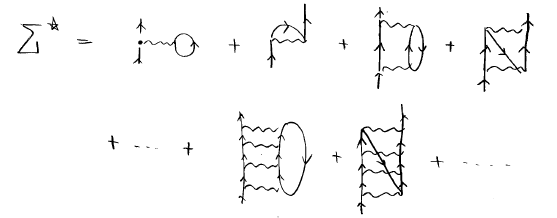
\includegraphics[width=0.8\textwidth]{2-7-13.png}\label{Fig2.7.13}
\end{center}

These ladder-type of diagram can be given by so-called the effective two-particle interaction.
\begin{center}
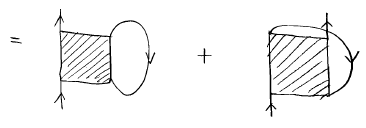
\includegraphics[width=0.55\textwidth]{2-7-13'.png}\label{Fig2.7.13'}
\begin{equation} \label{Eqs2.7.4}\end{equation}
\end{center}

Where the effective two-particle interaction is given by this:
\begin{center}
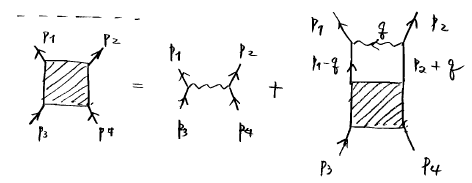
\includegraphics[width=0.6\textwidth]{2-7-14.png}\label{Fig2.7.14}
\begin{equation} \label{Eqs2.7.5}\end{equation}
\end{center}
\begin{center}---------------------------------------------\end{center}
The corresponding analytic expression are given as follows:
\begin{equation*} \label{Eqs2.7.4'} \tag{2.7.4'} \hbar\Sigma^{\bigstar}(p) = -2 i \frac{1}{(2\pi)^4} \int \mathrm{d}^4 k G^0(k) \Gamma(p,k;p,k)+i \frac{1}{(2\pi)^4}\int \mathrm{d}^4 k G^0(k) \Gamma(k,p;p,k) \end{equation*}
\begin{equation} \label{Eqs2.7.6} \begin{split}
\Gamma(p_1,p_2;p_3,p_4) = v_0(p_1-p_3) + &i \hbar^{-1} \frac{1}{(2\pi)^4} \int \mathrm{d}^4 q v_0(q) \\
&\times G^0(p_1-q)G^0(p_2+q)\Gamma(p_1-q,p_2+q;p_3,p_4)
\end{split}\end{equation}

with $v_0(q) = V_0(\mathbf{q})$

This factor ``2" comes from the summation over spin index associated with this closed loop, while the corresponding spin index here is fixed by the external line so that there is no factor ``2" in the 2nd term. The minus sign here comes from this closed loop, while there is no closed loop in the 2nd term.

This self consistent equation for the two-particle interaction is called Bethe-Salpeter equation, for the effective interaction.

Now, the calculation of the proper self energy reduces to solving the Bethe-Salpeter equation in favor for the effective interaction.

To do this, let us define an ``effective wavefunction" $Q$ out of the effective interaction.
\begin{equation} \label{Eqs2.7.7}
\Gamma(p_1,p_2;p_3,p_4) \equiv \frac{1}{(2\pi)^4} \int \mathrm{d}^4 q v_0(q) Q(p_1-q,p_2+q;p_3,p_4)
\end{equation}

The B.S. equation for the effective wavefunction is given by\footnote{\[ \begin{split} \Gamma(p_1,p_2;p_3,p_4) =& (2\pi)^{-4} \int \mathrm{d}^4 q v_0(q) (2\pi)^4 \delta(p_1-q-p_3) \\&+ (2\pi)^{-4} \int \mathrm{d}^4 q v_0(q) \frac{i}{\hbar}G^0(p_1-q)G^0(p_2+q)\Gamma(p_1-q,p_2+q;p_3,p_4) \end{split} \]}:
\begin{equation} \label{Eqs2.7.8}
Q(p_1,p_2;p_3,p_4) = (2\pi)^4 \delta^4(p_1-p_3) + \left(\frac{i}{\hbar}\right) G^0(p_1)G^0(p_2) \times \int \frac{\mathrm{d}^4 q}{(2\pi)^4} v_0(q)\cdot Q(p_1-q,p_2+q;p_3,p_4)
\end{equation}

To study this B.S. equation, let us first introduce the total center of mass wave vector as
\begin{equation} \label{Eqs2.7.9} P \equiv p_1+p_2 = p_3 + p_4 \end{equation}

where the last equality comes from the conservation of total four-momentum.

We also introduce the relative wave vectors as
\begin{equation} \label{Eqs2.7.10} p \equiv \frac{1}{2}(p_1-p_2), p^{'} \equiv \frac{1}{2}(p_3-p_4) \end{equation}

In terms of these three wave vectors, $p_1,p_2,p_3,p_4$ are given as follows.
\begin{equation} \label{Eqs2.7.11} \left \{ \begin{split} &p_1 = \frac{1}{2}P+p, p_2 = \frac{1}{2}P-p \\ &p_3 = \frac{1}{2}P+p^{'} , p_4 = \frac{1}{2}P-p^{'}
\end{split} \right. \end{equation}

Let us integrate $Q(p_1,p_2;p_3,p_4)$ over the frequency component of the former relative wave vector $(p)$:\footnote{$p \equiv (\mathbf{p},p_0), p^{'} \equiv (\mathbf{p}^{'},p_0^{'})$}
\begin{equation} \label{2.7.12} \begin{split}
\frac{1}{2\pi} \int \mathrm{d}p_0 Q(p_1,p_2;p_3,p_4) =
& \frac{1}{2\pi} \int \mathrm{d}p_0 Q(\frac{1}{2}P+p,\frac{1}{2}P-p;\frac{1}{2}P+p^{'},\frac{1}{2}P-p^{'})\\
\equiv & \chi(\mathbf{p},p^{'},P)
\end{split}\end{equation}

which we call as $\chi(\mathbf{p},p^{'},P)$.

Now that $v_0(q)$ is independent of the frequency component of $q$: $v_0(q) \equiv V_0(\mathbf{q})$, the B.S. equation for $Q$ can be made into that for $\chi$.

Namely, this part reduces to this\footnote{$q \equiv (\mathbf{q},q_0)$}:
\[ \int \frac{\mathrm{d}^4 q}{(2\pi)^4} v_0(q) Q(p_1-q,p_2+q;p_3,p_4) = \int \frac{\mathrm{d}^3 \mathbf{q}}{(2\pi)^3} V_0(\mathbf{q}) \chi(\mathbf{p}-\mathbf{q}, p^{'}, P) \]

So that, by integrating over $p_0$, we can reduce this B.S. equation into this:
\[ \begin{split}
&\int \frac{\mathrm{d}p_0}{2\pi} Q(\frac{1}{2}P+p,\frac{1}{2}P-p;\frac{1}{2}P+p^{'},\frac{1}{2}P-p^{'})\\
= &\int \frac{\mathrm{d}p_0}{2\pi} (2\pi)^4 \delta^4(p-p^{'}) + i \hbar^{-1} \int \frac{\mathrm{d}p_0}{2\pi} G^0(\frac{1}{2}P+p)G^0(\frac{1}{2}P-p) \times \int \frac{\mathrm{d}^3\mathbf{q}}{(2\pi)^3} V_0(\mathbf{q})\chi(\mathbf{p}-\mathbf{q},p^{'},P)\\
=&(2\pi)^3 \delta^3(\mathbf{p}-\mathbf{p}^{'}) + i \hbar^{-1} \int \frac{\mathrm{d}p_0}{2\pi} G^0(\frac{1}{2}P+p)G^0(\frac{1}{2}P-p) \times \int \frac{\mathrm{d}^3\mathbf{q}}{(2\pi)^3} V_0(\mathbf{q})\chi(\mathbf{p}-\mathbf{q},p^{'},P)
\end{split} \]

Namely, we obtain the B.S. equation for $\chi$:
\begin{equation} \label{Eqs2.7.13}
\chi(\mathbf{p},p^{'},P) = (2\pi)^3 \delta^3(\mathbf{p}-\mathbf{p}^{'}) + \frac{i}{\hbar} \int \frac{\mathrm{d}p_0}{2\pi} G^0(\frac{1}{2}P+p)G^0(\frac{1}{2}P-p)\times\int\frac{\mathrm{d}^3 \mathbf{q}}{(2\pi)^3}V_0(\mathbf{q}) \chi(\mathbf{p}-\mathbf{q},p^{'},P)
\end{equation}

When solving this equation iteratively, one can see that $\chi(\mathbf{p},p^{'},P)$ thus given is actually independent from the frequency component of $p^{'}$:
\[ \begin{split} \chi(\mathbf{p},p^{'},P) =& (2\pi)^3\delta^3(\mathbf{p}-\mathbf{p}^{'})+\frac{i}{\hbar} \int \frac{\mathrm{d}p_0}{2\pi}G^0(\frac{1}{2}P+p)G^0(\frac{1}{2}P-p)V_0(\mathbf{p}-\mathbf{p}^{'})\\
&+\left(\frac{i}{\hbar}\right)^2 \int \frac{\mathrm{d}p_0}{2\pi}G^0(\frac{1}{2}P+p)G^0(\frac{1}{2}P-p) \\
&\quad \times \frac{1}{(2\pi)^3} \int \mathrm{d}^3\mathbf{q}V_0(\mathbf{q}) \int \frac{\mathrm{d}(p_0-q_0)}{2\pi}G^0(\frac{1}{2}P+p-q)G^0(\frac{1}{2}P-p+q)V_0(\mathbf{p}-\mathbf{q}-\mathbf{p}^{'})\\
&+ \ldots
\end{split} \]

Thus, we just call $\chi(\mathbf{p},p^{'},P)$ as $\chi(\mathbf{p},\mathbf{p}^{'},P)$.
\begin{equation} \label{Eqs2.7.14}
\chi(\mathbf{p},\mathbf{p}^{'},P) = (2\pi)^3 \delta^3(\mathbf{p}-\mathbf{p}^{'}) + \underline{\frac{i}{\hbar} \int \frac{\mathrm{d}p_0}{2\pi} G^0(\frac{P}{2}+p)G^0(\frac{P}{2}-p)}\times\int\frac{\mathrm{d}^3 \mathbf{q}}{(2\pi)^3}V_0(\mathbf{q}) \chi(\mathbf{p}-\mathbf{q},\mathbf{p}^{'},P)
\end{equation}

It is now easy to evaluate the underlined part:
\[\begin{split} =& \frac{i}{\hbar} \int \frac{\mathrm{d}p_0}{2\pi} \left[ \frac{\theta(|\frac{\mathbf{P}}{2}+\mathbf{p}|-k_F)}{\hbar(\frac{P_0}{2}+p_0)-\epsilon_{\frac{\mathbf{P}}{2}+\mathbf{p}}+i\eta} + \frac{\theta(k_F-|\frac{\mathbf{P}}{2}+\mathbf{p}|)}{\hbar(\frac{P_0}{2}+p_0)-\epsilon_{\frac{\mathbf{P}}{2}+\mathbf{p}}-i\eta} \right] \\
& \times \left[ \frac{\theta(|\frac{\mathbf{P}}{2}-\mathbf{p}|-k_F)}{\hbar(\frac{P_0}{2}-p_0)-\epsilon_{\frac{\mathbf{P}}{2}-\mathbf{p}}+i\eta} + \frac{\theta(k_F-|\frac{\mathbf{P}}{2}-\mathbf{p}|)}{\hbar(\frac{P_0}{2}-p_0)-\epsilon_{\frac{\mathbf{P}}{2}-\mathbf{p}}-i\eta} \right]\\
=& i (-i) \left[ \frac{\theta(|\frac{\mathbf{P}}{2}+\mathbf{p}|-k_F)\theta(|\frac{\mathbf{P}}{2}-\mathbf{p}|-k_F)}{\hbar P_0 - \epsilon_{\frac{\mathbf{P}}{2}+\mathbf{p}} - \epsilon_{\frac{\mathbf{P}}{2}-\mathbf{p}} + 2i\eta} - \frac{\theta(k_F-|\frac{\mathbf{P}}{2}+\mathbf{p}|)\theta(k_F-|\frac{\mathbf{P}}{2}-\mathbf{p}|)}{\hbar P_0 - \epsilon_{\frac{\mathbf{P}}{2}+\mathbf{p}} - \epsilon_{\frac{\mathbf{P}}{2}-\mathbf{p}} - 2i\eta} \right]
\end{split} \]

Now that $\epsilon_\mathbf{k} \equiv \frac{\hbar^2\mathbf{k}^2}{2m}$, we have
\begin{equation*} \label{Eqs2.7.15'}\hbar P_0 - \epsilon_{\frac{1}{2}\mathbf{P}+\mathbf{p}}- \epsilon_{\frac{1}{2}\mathbf{P}-\mathbf{p}} = \hbar P_0 - \frac{\hbar^2\mathbf{P}^2}{4m}-\frac{\hbar^2\mathbf{p}^2}{m}=E-\frac{\hbar^2\mathbf{p}^2}{m}\tag{2.7.15'}\end{equation*}

Using also
\begin{equation} \label{Eqs2.7.15}
N(\mathbf{P},\mathbf{p}) = 1-n^0_{\frac{\mathbf{P}}{2}+\mathbf{p}}-n^0_{\frac{\mathbf{P}}{2}-\mathbf{p}} \end{equation}

with $n_\mathbf{p}^0 \equiv \theta(k_F-|\mathbf{p}|)$, the underlined part can be simplified into this:
\[ \frac{i}{\hbar} \int \frac{\mathrm{d}p_0}{2\pi}G^0(\frac{P}{2}+p)G^0(\frac{P}{2}-p) = \frac{N(\mathbf{P},\mathbf{p})}{E-\frac{\hbar^2\mathbf{p}^2}{m}+i\eta N(\mathbf{P},\mathbf{p})} \]

and B.S. equation can be given as follows:
\begin{equation} \label{Eqs2.7.16}
\chi(\mathbf{p},\mathbf{p}^{'},P) = (2\pi)^3 \delta^3(\mathbf{p}-\mathbf{p}^{'}) + \frac{N(\mathbf{P},\mathbf{p})}{E-\frac{\hbar^2\mathbf{p}^2}{m}+i\eta N(\mathbf{P},\mathbf{p})}\int \frac{\mathrm{d}^3 \mathbf{q}}{(2\pi)^3} \times V_0(\mathbf{q})\chi(\mathbf{p}-\mathbf{q},\mathbf{p}^{'},P) \end{equation}

In terms of $\chi$ thus given, the effective two-particle interaction is given as follows:
\begin{equation} \label{Eqs2.7.17}
\Gamma(\mathbf{p},\mathbf{p}^{'},P) = \frac{1}{(2\pi)^3} \int \mathrm{d}^3 \mathbf{q} V_0(\mathbf{q}) \chi(\mathbf{p}-\mathbf{q},\mathbf{p}^{'},P) \end{equation}

To solve this Bethe-Salpeter equation, let us first consider the low density limit, in which $N(\mathbf{P},\mathbf{p})$ can be replaced by $1$.
\begin{equation} \label{Eqs2.7.18}
\chi_0(\mathbf{p},\mathbf{p}^{'},P) = (2\pi)^3 \delta^3(\mathbf{p}-\mathbf{p}^{'}) + \frac{1}{E-\frac{\hbar^2\mathbf{p}^2}{m}+i\eta}\times \int \frac{\mathrm{d}^3\mathbf{q}}{(2\pi)^3}V_0(\mathbf{q})\chi_0(\mathbf{p}-\mathbf{q},\mathbf{p}^{'},P) \end{equation}

By scaling $E$ and $V_0$ by $\frac{\hbar^2}{m}$,
\begin{equation} \label{Eqs2.7.19}
\epsilon = \frac{mE}{\hbar^2}, v_0(\mathbf{q}) = \frac{m V_0(\mathbf{q})}{\hbar^2} \end{equation}

we have:
\begin{equation*} \label{Eqs2.7.18'} \tag{2.7.18'}
\chi_0(\mathbf{p},\mathbf{p}^{'},P) = (2\pi)^3\delta^3(\mathbf{p}-\mathbf{p}^{'}) + \frac{1}{\epsilon-\mathbf{p}^2+i\eta}\times\int\frac{\mathrm{d}^3\mathbf{q}}{(2\pi)^3}v_0(\mathbf{q}) \chi_0(\mathbf{p}-\mathbf{q},\mathbf{p}^{'},P)
\end{equation*}

This equation can be solved closely in paralled to the scattering problem of one electron by a sperical hard core potential.

\begin{center}---------------------\end{center}

I suppose that the scattering problem are usually given in the course of Quantum Mechanics, so that I will not go into the details of it. But, to make this class to be self-contained, I will briefly summarize the scattering problem of single electron by the hard core potential.

Consider that an incident electron wave of momentum $\mathbf{k}$ is injected to a spherical hard core potential:
\begin{equation*} \label{Eqs2.7.A.1} \tag{2.7.A.1}
\left[ -\frac{\hbar^2\nabla^2}{2m}+ V(\mathbf{x}) \right] \psi(\mathbf{x}) = E \psi(\mathbf{x})
\end{equation*}

where $V(\mathbf{x})$ represent the hard core potential depending only on the radial coordinate.
\begin{center} 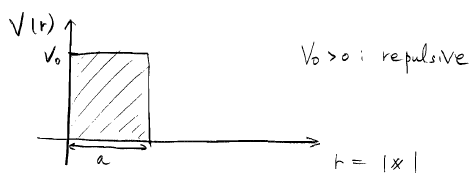
\includegraphics[width=0.5\textwidth]{2-7-15.png} \label{Fig2.7.15} \end{center}

Since the incident wave have momentum $\mathbf{k}$, we want find an eigenstate of this Hamiltonian which have energy of $\frac{\hbar^2\mathbf{k}^2}{2m}$.

With a proper scaling, this reduces to
\begin{equation*} \label{Eqs2.7.A.1'} \tag{2.7.A.1'}
\left[ \nabla^2+ |\mathbf{k}|^2) \right] \psi(\mathbf{x}) = v(\mathbf{x}) \psi(\mathbf{x}) \qquad \left(v(\mathbf{x})=\frac{2mV(\mathbf{x})}{\hbar^2}\right)
\end{equation*}

When $\mathbf{x}$ is far from the origin at which the hard core scattering potential is located, the eigenwavefunction become a plane-wave with the momentum $\mathbf{k}$.
\[ \psi(\mathbf{x}) = \mathrm{e}^{i \mathbf{k}\cdot \mathbf{x}} + \ldots \]

Since this requirement is nothing but the boundary condition, we put $\mathbf{k}$ as a subscript of $\psi$:
\[ \psi_\mathbf{k}(\mathbf{x}) = \mathrm{e}^{i \mathbf{k}\cdot \mathbf{x}} + \ldots \]

When $\mathbf{x}$ becomes close to the scattering potential, we need correction to the eigenwavefunction, which can be given like this:
\begin{equation*} \label{Eqs2.7.A.2} \tag{2.7.A.2} \psi_\mathbf{k}(\mathbf{x}) = \mathrm{e}^{i \mathbf{k}\cdot \mathbf{x}} - \int \mathrm{d}^3 \mathbf{y} G^{(+)}(\mathbf{x}-\mathbf{y}) v(\mathbf{y}) \psi_{\mathbf{k}}(\mathbf{y})
\end{equation*}

An ``out-going-wave" Green's function $G^{(+)}$ which satisfies this:
\begin{equation*} \label{Eqs2.7.A.3} \tag{2.7.A.3}
\left( \nabla_{\mathbf{x}}^2 + {|\mathbf{k}|}^2 \right) G^{(+)}(\mathbf{x}-\mathbf{y}) = - \delta^3 (\mathbf{x}-\mathbf{y}) \end{equation*}

is given by this:
\begin{equation*} \label{Eqs2.7.A.4} \tag{2.7.A.4}
G^{(+)}(\mathbf{x}-\mathbf{y}) = \int \frac{\mathrm{d}^3 \mathbf{p}}{(2 \pi)^3} \frac{\mathrm{e}^{i \mathbf{p} \cdot (\mathbf{x}-\mathbf{y})}}{p^2-k^2-i \eta}
= \frac{1}{4 \pi} \frac{\mathrm{e}^{i k |\mathbf{x}-\mathbf{y}|}}{|\mathbf{x}-\mathbf{y}|}
\end{equation*}

You can check that this set of solutions indeed satisfies this Schr\"odinger equation.

If the scattering potential has no bound state, then this eigenstate support a complete set of states:
\begin{equation*} \label{Eqs2.7.A.5} \tag{2.7.A.5}
\int \frac{\mathrm{d}^3 \mathbf{k}}{(2\pi)^3} \psi_{\mathbf{k}} (\mathbf{x}) \psi_{\mathbf{k}}^* (\mathbf{k}^{'}) = \delta^3 (\mathbf{x}-\mathbf{x}^{'})
\end{equation*}

In the momentum representation,
\begin{equation*} \label{Eqs2.7.A.6} \tag{2.7.A.6}
\left\{ \begin{split}
\psi_{\mathbf{k}} (\mathbf{p}) &\equiv \int \mathrm{d}^3 \mathbf{x} \mathrm{e}^{-i \mathbf{p} \cdot \mathbf{x}} \psi_{\mathbf{k}} (\mathbf{x})\\
v(\mathbf{p}) & \equiv \int \mathrm{d}^3 \mathbf{x} \mathrm{e}^{-i \mathbf{p} \cdot \mathbf{x}} v(\mathbf{x})
\end{split} \right.
\end{equation*}

This equation can be rewritten as
\begin{equation*} \label{Eqs2.7.A.7} \tag{2.7.A.7}
\psi_{\mathbf{k}}(\mathbf{p}) = (2\pi) ^3 \delta^3(\mathbf{k}-\mathbf{p}) - \frac{1}{\mathbf{p}^2 - \mathbf{k}^2 - i \eta} \int \frac{ \mathrm{d}^3 \mathbf{q}}{(2\pi)^3} v(\mathbf{q}) \psi_{\mathbf{k}}(\mathbf{p}-\mathbf{q})
\end{equation*}

Then the scattering amplitude for a transition from an incident wave vector $\mathbf{k}$ to a final wave vector $\mathbf{p}$ is defined by this part:
\begin{equation*} \label{Eqs2.7.A.8} \tag{2.7.A.8}
\tilde{f}(\mathbf{p},\mathbf{k}) \equiv -4 \pi f(\mathbf{p},\mathbf{k}) \equiv \int \frac{\mathrm{d}\mathbf{q}}{(2\pi)^3} v(\mathbf{q}) \psi_{\mathbf{k}}(\mathbf{p}-\mathbf{q})
\end{equation*}

In terms of the scattering amplitude, this reduces to this:
\begin{equation*} \label{Eqs2.7.A.7'} \tag{2.7.A.7'}
\psi_{\mathbf{k}} (\mathbf{p}) = (2\pi)^3 \delta^3(\mathbf{k}-\mathbf{p}) + \frac{\tilde{f}(\mathbf{p},\mathbf{k})}{k^2-p^2+i \eta}
\end{equation*}

According to this completeness relation, this satisfies the corresponding completeness relation, which is given like this:
\begin{equation*} \label{Eqs2.7.A.9} \tag{2.7.A.9}
\int \frac{\mathrm{d}^3 \mathbf{k}}{(2\pi)^3} \psi_{\mathbf{k}}(\mathbf{p}) \psi_{\mathbf{k}}^* (\mathbf{p}^{'}) = (2\pi) ^3 \delta^3 (\mathbf{p} - \mathbf{p}^{'})
\end{equation*}

When the norm of the outgoing-wave momentum($|\mathbf{k}| = |\mathbf{k}^{'}|$) and that of the incident wave is same, the scattering amplitude is calculated by ``the method of partial wave":\footnote{$\mathrm{P}_l(x)$ is the Legendre polynomial.}
\begin{equation*} \label{Eqs2.7.A.10} \tag{2.7.A.10}
f(\mathbf{k},\mathbf{k}^{'}) = \sum_{l=0}^{\infty} \frac{2l+1}{k} \mathrm{e}^{i \delta_l} sin(\delta_l) \mathrm{P}_l (cos\theta)
\end{equation*}

where $\theta$ is angle subtended by $\mathbf{k}$ and $\mathbf{k}^{'}$ and $k = |\mathbf{k}| = |\mathbf{k}^{'}|$.

$\delta_l$ is called a ``phase shift" associated with $l$-th partial wave.

In the limit of hard core($V_0 \rightarrow +\infty$), the phase shift can be expanded with respect to small $k_a$, as:\footnote{see eq.( 19.21) in the text book by L.Schiff ``Quantum Mechanics" (3rd edition).}
\begin{equation*} \label{Eqs2.7.A.11} \tag{2.7.A.11}
tan(\delta_l) = - \frac{(k_a)^{2l+1}}{(2l+1)[(2l-1)!!]^2} + o((k_a)^{2l+2})\end{equation*}

\begin{center}-----------------------------------\end{center}

These are the summary of ``scattering problem of a single electron by a spherical hard core potential", which becomes very useful for solving the Bethe-Salpeter equation in the low-density limit.

\begin{equation*}  \tag{2.7.18'}
\chi_0(\mathbf{p},\mathbf{p}^{'},P) = (2\pi)^3\delta^3(\mathbf{p}-\mathbf{p}^{'}) + \frac{1}{\epsilon-\mathbf{p}^2+i\eta}\cdot\int\frac{\mathrm{d}^3\mathbf{q}}{(2\pi)^3}v_0(\mathbf{q}) \chi_0(\mathbf{p}-\mathbf{q},\mathbf{p}^{'},P)
\end{equation*}

To see this, let us rewrite this as follows
\begin{equation*} \label{Eqs2.7.18''} \tag{2.7.18''}
\begin{split}
(\epsilon-\mathbf{p}^2+i\eta)\chi_0(\mathbf{p},\mathbf{p}^{'},P) - \int\frac{\mathrm{d}^3\mathbf{q}}{(2\pi)^3}v_0(\mathbf{q}) \chi_0(\mathbf{p}-\mathbf{q},\mathbf{p}^{'},P)
&=(2\pi)^3 (\epsilon-\mathbf{p}^2+i\eta) \delta^3(\mathbf{p}-\mathbf{p}^{'})\\
&=(2\pi)^3 (\epsilon-{\mathbf{p}^{'}}^2+i\eta) \delta^3(\mathbf{p}-\mathbf{p}^{'})\end{split}
\end{equation*}

This equation can be satisfied by
\begin{equation} \label{Eqs2.7.20}
\chi_0(\mathbf{p},\mathbf{p}^{'},P) = (\epsilon - {\mathbf{p}^{'}}^2 + i \eta) \int \frac{\mathrm{d}\mathbf{k}}{(2\pi)^3} \frac{\psi_{\mathbf{k}}(\mathbf{p})\psi_{\mathbf{k}^{'}}^{*} (\mathbf{p}^{'})}{\epsilon - \mathbf{k}^2 + i \eta}
\end{equation}

where $\psi_{\mathbf{k}}(\mathbf{p})$ is given by eq.(\ref{Eqs2.7.A.7}), a solution of scattering problem of a single electron by hard core spherical potential.

Here the scattering potential $V(\mathbf{x})$ is replaced by the interaction potential between two particles $V_0(\mathbf{x})$
\begin{equation} \label{Eqs2.7.21}
\left\{ \begin{split} V(\mathbf{x}) &\rightarrow V_0(\mathbf{x})\\ v(\mathbf{q}) &\rightarrow v_0(\mathbf{q})
\end{split} \right.
\end{equation}

With this replacement in mind, we then recycle all the results obtained in the scattering problem here.

By the way, one can easily see this:
\[ \begin{split}
(\epsilon-\mathbf{p}^2+i\eta)\chi_0(\mathbf{p},\mathbf{p}^{'},P) =& (\epsilon-{\mathbf{p}^{'}}^2+i\eta)\int \frac{\mathrm{d}^3 \mathbf{k}}{(2\pi)^3}\frac{(\epsilon-\mathbf{p}^2+i\eta)\psi_{\mathbf{k}}(\mathbf{p})\psi_{\mathbf{k}}^{*}(\mathbf{p}^{'})}{\epsilon-\mathbf{k}^2+i\eta}\\
=&(\epsilon-{\mathbf{p}^{'}}^2+i\eta)\int \frac{\mathrm{d}^3 \mathbf{k}}{(2\pi)^3}\psi_{\mathbf{k}}(\mathbf{p})\psi_{\mathbf{k}}^{*}(\mathbf{p}^{'})\\
&+(\epsilon-{\mathbf{p}^{'}}^2+i\eta)\int \frac{\mathrm{d}^3 \mathbf{k}}{(2\pi)^3}\frac{(\mathbf{k}^2-\mathbf{p}^2+i \eta)\psi_{\mathbf{k}}(\mathbf{p})\psi_{\mathbf{k}}^{*}(\mathbf{p}^{'})}{\epsilon-\mathbf{k}^2+i\eta}\\
=&(\epsilon-{\mathbf{p}^{'}}^2+i\eta)\delta^3(\mathbf{p}-\mathbf{p}^{'})\\
&+(\epsilon-{\mathbf{p}^{'}}^2+i\eta)\int \frac{\mathrm{d}^3 \mathbf{k}}{(2\pi)^3}\int \frac{\mathrm{d} \mathbf{q}}{(2\pi)^3} \frac{v(\mathbf{q})\psi_{\mathbf{k}}(\mathbf{p}-\mathbf{q})\psi_{\mathbf{k}}^{*}(\mathbf{p}^{'})}{\epsilon - \mathbf{k}^2+i \eta}\\
=&(\epsilon-{\mathbf{p}^{'}}^2+i\eta)\delta^3(\mathbf{p}-\mathbf{p}^{'})+\int \frac{\mathrm{d} \mathbf{q}}{(2\pi)^3} N(\mathbf{q}) \chi_0(\mathbf{p}-\mathbf{q},\mathbf{p}^{'},P)
\end{split} \]

Using (\ref{Eqs2.7.A.7'}), this can be rewritten as:
\begin{equation} \label{Eqs2.7.22} \begin{split}
\chi_0(\mathbf{p},\mathbf{p}^{'},P) =& (\epsilon-{\mathbf{p}^{'}}^2+i\eta)\int \frac{\mathrm{d}^3 \mathbf{k}}{(2\pi)^3}\frac{\psi_{\mathbf{k}}(\mathbf{p})\psi_{\mathbf{k}}^{*}(\mathbf{p}^{'})}{\epsilon-\mathbf{k}^2+i \eta}\\
=&(\epsilon-{\mathbf{p}^{'}}^2+i\eta)\int \frac{\mathrm{d}^3 \mathbf{k}}{(2\pi)^3}\frac{\psi_{\mathbf{k}}(\mathbf{p})}{\epsilon-\mathbf{k}^2+i \eta} \times \left\{ (2\pi)^3\delta^3(\mathbf{p}^{'}-\mathbf{k})+\frac{\tilde{f}^{*}(\mathbf{p}^{'},\mathbf{k})}{\mathbf{k}^2-{\mathbf{p}^{'}}^2-i \eta} \right\}\\
=&\psi_{\mathbf{p}^{'}}(\mathbf{p}) + \int \frac{\mathrm{d}^3 \mathbf{k}}{(2\pi)^3} \psi_{\mathbf{k}}(\mathbf{p}) \times \frac{\epsilon-{\mathbf{p}^{'}}^2+i \eta}{[\epsilon-\mathbf{k}^2+i \eta][\mathbf{k}^2-{\mathbf{p}^{'}}^2-i \eta]}\tilde{f}^{*}(\mathbf{p}^{'},\mathbf{k})\\
=&\psi_{\mathbf{p}^{'}}(\mathbf{p}) + \int \frac{\mathrm{d}^3 \mathbf{k}}{(2\pi)^3} \psi_{\mathbf{k}}(\mathbf{p}) \times \left[ \frac{1}{\epsilon-\mathbf{k}^2+2i \eta} + \frac{1}{\mathbf{k}^2-{\mathbf{p}^{'}}^2-i \eta} \right]\tilde{f}^{*}(\mathbf{p}^{'},\mathbf{k})
\end{split} \end{equation}

substituting this into eq.(\ref{Eqs2.7.17}), we finally obtain:
\begin{equation} \label{Eqs2.7.23} \begin{split}
\Gamma_0(\mathbf{p},\mathbf{p}^{'},P) =& \frac{1}{(2\pi)^3} \frac{\hbar^2}{m} \int \mathrm{d}^3\mathbf{q} v_0(\mathbf{q}) \chi_0(\mathbf{p}-\mathbf{q},\mathbf{p}^{'},P)\\
\frac{m}{\hbar^2}\Gamma_0(\mathbf{p},\mathbf{p}^{'},P) \xlongequal{\ref{Eqs2.7.22}}&\frac{1}{(2\pi)^3} \int \mathrm{d}^3 \mathbf{q} v_0(\mathbf{q}) \psi_{\mathbf{p}^{'}}(\mathbf{p}-\mathbf{q})\\
&+ \frac{1}{(2\pi)^3} \int \mathrm{d}^3 \mathbf{q} v_0(\mathbf{q}) \int \frac{\mathrm{d}^3\mathbf{k}}{(2\pi)^3} \psi_{\mathbf{k}}(\mathbf{p}-\mathbf{q})\left[ \frac{1}{\epsilon-\mathbf{k}^2+i \eta} + \frac{1}{\mathbf{k}^2-{\mathbf{p}^{'}}^2-i \eta} \right] \tilde{f}^{*}(\mathbf{p}^{'},\mathbf{k})\\
\xlongequal{\ref{Eqs2.7.A.8}}& \tilde{f}(\mathbf{p},\mathbf{p}^{'}) + \int \frac{\mathrm{d}^3 \mathbf{k}}{(2\pi)^3} \tilde{f}(\mathbf{p},\mathbf{k})\left[ \frac{1}{\epsilon-\mathbf{k}^2+i \eta} + \frac{1}{\mathbf{k}^2-{\mathbf{p}^{'}}^2-i \eta} \right] \times \tilde{f}^{*}(\mathbf{p}^{'},\mathbf{k})
\end{split}\end{equation}

This expression suggests that the effective two particle interaction in the low density limit can be expressed only by the scattering amplitude $\tilde{f}(\mathbf{k},\mathbf{k}^{'})$, which is calculated from the scattering problem of a single electron.

We now try to solve eq.(\ref{Eqs2.7.16}) for finite $N(\mathbf{P},\mathbf{p})$.
\begin{equation*} \label{Eqs2.7.16'} \tag{2.7.16'}
\chi(\mathbf{p},\mathbf{p}^{'},P)=(2\pi)^3 \delta^3(\mathbf{p}-\mathbf{p}^{'}) + \frac{N(\mathbf{P},\mathbf{p})}{\epsilon - p^2 + i \eta N(\mathbf{P},\mathbf{p})} \int \frac{\mathrm{d}^3\mathbf{q}}{(2\pi)^3}v(\mathbf{q})\chi(\mathbf{p}-\mathbf{q},\mathbf{p}^{'},P)
\end{equation*}

\[\int \frac{\mathrm{d}^3\mathbf{p}^{'}}{(2\pi)^3}\left[ (2\pi)^3 \delta^3(\mathbf{p}-\mathbf{p}^{'})-\frac{v(\mathbf{p}-\mathbf{p}^{'})}{\epsilon-\mathbf{p}^2+i \eta} \right] \chi_0(\mathbf{p}^{'},\mathbf{p}^{''},P) = (2\pi)^3 \delta^3(\mathbf{p}-\mathbf{p}^{'}) \]

\[ \int \mathrm{d}^3 \mathbf{p}^{'} \chi_0^{-1}(\mathbf{p},\mathbf{p}^{'},P)\chi_0(\mathbf{p}^{'},\mathbf{p}^{'},P) = (2\pi)^3 \delta^3(\mathbf{p}-\mathbf{p}^{'})\]

Thus
\[ \chi_0^{-1}(\mathbf{p},\mathbf{p}^{'},P) = \delta^3(\mathbf{p}-\mathbf{p}^{'}) - \frac{N(\mathbf{p}-\mathbf{p}^{'})}{\epsilon-\mathbf{p}^2+i \eta} \frac{1}{(2\pi)^3} \]

\[ \int \mathrm{d}^3 \mathbf{p} \chi_0(\mathbf{p}^{''},\mathbf{p},P)\chi_0^{-1}(\mathbf{p},\mathbf{p}^{'},P) = (2\pi)^3 \delta^3(\mathbf{p}^{''}-\mathbf{p}^{'})\]

We first substract the eq in the low density limit:
\[ \begin{split} &\chi(\mathbf{p},\mathbf{p}^{'},P) - \frac{1}{\epsilon-\mathbf{p}^2+i \eta} \int \frac{\mathrm{d}^3 \mathbf{q}}{(2\pi)^3} v(\mathbf{q}) \chi(\mathbf{p}-\mathbf{q},\mathbf{p}^{'},P)\\
&=(2\pi)^3 \delta(\mathbf{p}-\mathbf{p}^{'}) + \left( \frac{N(\mathbf{P},\mathbf{p})}{\epsilon - \mathbf{p}^2+i \eta N(\mathbf{P},\mathbf{p})} - \frac{1}{\epsilon - \mathbf{p}^2+i \eta} \right)\times \underline{\int \frac{\mathrm{d}^3 \mathbf{q}}{(2\pi)^3} v(\mathbf{q})\chi(\mathbf{p}-\mathbf{q},\mathbf{p}^{'},P)}
\end{split} \]

where the underlined part can be replaced by the effective two-particle interaction $\frac{m}{\hbar^2}\Gamma(\mathbf{p},\mathbf{p}^{'},P)$.
\[ \begin{split} &\int \mathrm{d}^3 \mathbf{p}^{''} \chi_0^{-1}(\mathbf{p},\mathbf{p}^{''},P)\chi(\mathbf{p}^{''},\mathbf{p}^{'},P)\\
&=(2\pi)^3 \delta^3(\mathbf{p}-\mathbf{p}^{'}) + \left( \frac{N(\mathbf{P},\mathbf{p})}{\epsilon - \mathbf{p}^2+i \eta N(\mathbf{P},\mathbf{p})} - \frac{1}{\epsilon - \mathbf{p}^2+i \eta} \right)\times\frac{m}{\hbar^2}\Gamma(\mathbf{p},\mathbf{p}^{'},P)
\end{split} \]

\[ \begin{split} &\int \mathrm{d}^3\mathbf{q} \chi_0(\mathbf{p},\mathbf{q},P) \int \mathrm{d}^3 \mathbf{p}^{''} \chi_0^{-1}(\mathbf{q},\mathbf{p}^{''},P)\chi(\mathbf{p}^{''},\mathbf{p}^{'},P)\\
&= \int \mathrm{d}^3\mathbf{q}\chi_0(\mathbf{p},\mathbf{q},P)(2\pi)^3\delta^3(\mathbf{q}-\mathbf{p}^{'})\\&\quad+ \int \mathrm{d}^3 \mathbf{q} \chi_0(\mathbf{p},\mathbf{q},P) \left[ \frac{N(\mathbf{P},\mathbf{q})}{\epsilon - \mathbf{q}^2+i \eta N(\mathbf{P},\mathbf{q})} - \frac{1}{\epsilon - \mathbf{q}^2+i \eta} \right] \frac{m}{\hbar^2} \Gamma(\mathbf{q},\mathbf{p}^{'},P)
\end{split} \]


\[ \begin{split} \Leftrightarrow (2\pi)^3 \chi(\mathbf{p},\mathbf{p}^{'},P) =& (2\pi)^3\chi_0(\mathbf{p},\mathbf{p}^{'},P) \\
&+ \int \mathrm{d}^3 \mathbf{p}^{''} \chi_0(\mathbf{p},\mathbf{p}^{''},P) \left[ \frac{N(\mathbf{P},\mathbf{p}^{''})}{\epsilon - {\mathbf{p}^{''}}^2+i \eta N(\mathbf{P},\mathbf{p}^{''})} - \frac{1}{\epsilon - {\mathbf{p}^{''}}^2+i \eta} \right]\frac{m}{\hbar^2} \Gamma(\mathbf{p}^{''},\mathbf{p}^{'},P) \end{split}\]

\[ \begin{split} \chi(\mathbf{p},\mathbf{p}^{'},P) =& \chi_0(\mathbf{p},\mathbf{p}^{'},P) \\
&+ \int \frac{\mathrm{d}^3 \mathbf{k}}{(2\pi)^3} \chi_0(\mathbf{p},\mathbf{k},P) \times \left[ \frac{N(\mathbf{P},\mathbf{k})}{\epsilon - {\mathbf{k}}^2+i \eta N(\mathbf{P},\mathbf{k})} - \frac{1}{\epsilon - {\mathbf{k}}^2+i \eta} \right]\frac{m}{\hbar^2} \Gamma(\mathbf{k},\mathbf{p}^{'},P)\end{split}\]

Then, multiplying $v(\mathbf{q})$ and replacing $\mathbf{p}$ by $\mathbf{p}-\mathbf{q}$ and intergrating over $\mathbf{q}$, we can replace this by $\Gamma$ and these two by $\Gamma_0$ respectively.
\begin{equation} \label{Eqs2.7.24} \begin{split}
\Gamma(\mathbf{p},\mathbf{p}^{'},P) =& \Gamma_0(\mathbf{p},\mathbf{p}^{'},P) \\
&+ \int \frac{\mathrm{d}^3 \mathbf{k}}{(2\pi)^3} \Gamma_0(\mathbf{p},\mathbf{k},P) \times \left[ \frac{N(\mathbf{P},\mathbf{k})}{\epsilon - {\mathbf{k}}^2+i \eta N(\mathbf{P},\mathbf{k})} - \frac{1}{\epsilon - {\mathbf{k}}^2+i \eta} \right]\frac{m}{\hbar^2} \Gamma(\mathbf{k},\mathbf{p}^{'},P)
\end{split}\end{equation}

A set of these two equations gives effective two-particle potential $\Gamma$ in terms of the scattering amplitude $\tilde{f}$.

Importantly, this scattering amplitude $\tilde{f}$ can be calculated from a single-particle scattering problem due to a hard core spherical scattering potential, which corresponds to our short-range s-wave repulsive interaction potential.

This set of equation are called as Galitskii's integral equation.

For a low density Fermi gas, eq.(\ref{Eqs2.7.24}) can be solved iteratively as a power series in small $k_F a(\ll1)$. Namely, the integrand of the 2nd term vanishes, when the vectors $\frac{1}{2}\mathbf{P}+\mathbf{k}$ and $\frac{1}{2}\mathbf{P}-\mathbf{k}$ are both outside the Fermi sea.

In a `small-Fermi-sea' limit, the integral region of the momentum $\mathbf{k}$ is restricted, so that the 2nd term can be roughly estinated as
\[ \Gamma_0 \cdot k_F \cdot m \Gamma \frac{1}{\hbar^2} \]

Thus, the correction to $\Gamma$ due to the 2nd term can be shown to be subleading order:
\[ \frac{\Gamma-\Gamma_0}{\Gamma} = \frac{k_F m \Gamma_0}{\hbar} = k_F \tilde{f} \xlongequal{\ref{Eqs2.7.A.10} \& \ref{Eqs2.7.A.11}} k_F a \ll 1 \]

Before solving eq.(\ref{Eqs2.7.24}) iteratively, please also notice that, according to eq.(\ref{Eqs2.7.4'}), the full set of variable $\mathbf{p}$,$\mathbf{p}^{'}$,$P$ is not necessary.

Namely, all that is necessary is the proper self-energy, which is given by this:
\[ \hbar \Sigma^{\bigstar}(p) = -2 i \int \frac{\mathrm{d}^4 k}{(2\pi)^4} G^0(k)\Gamma(p,k;p,k) + i \int \frac{\mathrm{d}^4 k}{(2\pi)^4}G^0(k)\Gamma(k,p;p,k) \]

Using
\[ \left. \begin{split}
P =& p_1 + p_2 = p_3 + p_4\\
p =& \frac{1}{2}(p_1-p_2)\\
p^{'} =& \frac{1}{2}(p_3-p_4)
 \end{split} \right\} \ref{Eqs2.7.9} \& \ref{Eqs2.7.10} \& \ref{Eqs2.7.11} \]
we have
\[\Gamma(p_1,p_2;p_3,p_4) \rightarrow \Gamma(p,p^{'},P)\]

Thus
\[ \Gamma(p,k;p,k) \rightarrow \Gamma(p-k,p-k,\frac{p+k}{2}) = \Gamma(q,q,P) \]

where
\[ \begin{split} \frac{1}{2}(p-k) =& q\\ p+k =& P \end{split} \]

and
\[\Gamma(p,k;k,p) \rightarrow \Gamma(q,-q,P)\]

According to eq.(\ref{Eqs2.7.17}), $\Gamma$ does not depend on the frequency component of first two four-dimensional momentum vector, so that, we replace these $q$ by three-dimensional momentum $\mathbf{q}$.

\[\frac{1}{2}(\mathbf{p}-\mathbf{k})=\mathbf{q}, \mathbf{p}+\mathbf{k}=\mathbf{P},p_0+k_0=P_0
 \]

\begin{equation} \label{Eqs2.7.25}
\hbar \Sigma^{\bigstar}(p) = -2 i \int \frac{\mathrm{d}^4 k}{(2\pi)^4} G^0(k)\Gamma(\mathbf{q},\mathbf{q},P) + i \int \frac{\mathrm{d}^4 k}{(2\pi)^4} G^0(k)\Gamma(\mathbf{q},-\mathbf{q},P)
\end{equation}

Many of the physical quantities can be calculated from self-energy, which is now given by two-particle effective interaction with a particular set of its variables.

Namely, $\mathbf{q}$, $\mathbf{q}$ and $P$; or $\mathbf{q}$, $-\mathbf{q}$ and $P$.

Thus, we will calculate $\Gamma$ with these particular set of variables, iteratively as a power of small $k_F a$.

To be more specific, we will obtain $\Gamma$ to the 2nd order of $k_F a$.

Using eq.(\ref{Eqs2.7.23}) and eqs. (\ref{Eqs2.7.A.10}) \& (\ref{Eqs2.7.A.11}), we first obtain $\Gamma_0$ to the 2nd order in $k_F a$.

From eqs. (\ref{Eqs2.7.A.10}) \& (\ref{Eqs2.7.A.11}), the scattering amplitude can be expanded in small $k_F a$ as this, for the case with $|\mathbf{k}|=|\mathbf{k}^{'}|$.
\footnote{the underlined part: see eq. (\ref{Eqs2.7.A.11}).}
\[ \begin{split} f(\mathbf{k},\mathbf{k}^{'}) =& \sum_{l=0}^{+\infty} \frac{2l+1}{k} \mathrm{e}^{i \delta_l} sin \delta_l \mathrm{P}_l(cos\theta)\\
=& k^{-1} (1+i \delta_0) \delta_0 + \underline{o(k^{-1} \cdot (k a)^3)}\\
\xlongequal{\ref{Eqs2.7.A.11}}& -a + i k a^2 + o(k^2 a^3)
\end{split} \]
\[ \tilde{f}(\mathbf{k},\mathbf{k}^{'}) = 4\pi a - 4\pi i a^2 k + o(k^2 a^3) \]

Since $\tilde{f}$ is already at most 1st order in small $a$, we can replace $\tilde{f}$ in the 2nd term of eq.(\ref{Eqs2.7.23}) by its first order contribution, while replace $\tilde{f}$ in the first term of eq.(\ref{Eqs2.7.23}) by its expression up to the 2nd order.

Such treatment gives us $\Gamma_0$ to the 2nd order in small $a$:
\[ \begin{split} \frac{m}{\hbar^2} \Gamma_0(\mathbf{q},\mathbf{q},P) =& 4\pi a - 4\pi i q a^2 + \int \frac{\mathrm{d}^3 k^{'}}{(2\pi)^3} 4\pi a \left( \frac{1}{\epsilon-{k^{'}}^2 + i \eta} + \frac{1}{{k^{'}}^2-q^2-i \eta} \right)4\pi a + o(a^3)\\
=& 4\pi a - 4\pi i q a^2 + (4\pi a)^2 \times \int \frac{\mathrm{d}^3 k^{'}}{(2\pi)^3} \left( \frac{1}{\epsilon-{k^{'}}^2 + i \eta} + \frac{1}{{k^{'}}^2-q^2-i \eta} \right) + \ldots\\
=& 4\pi a - 4\pi i q a^2 + (4\pi a)^2 \times\\
&\int \frac{\mathrm{d}^3 k^{'}}{(2\pi)^3} \left( \frac{1}{\epsilon-{k^{'}}^2 + i \eta} + \frac{\mathscr{P}}{{\mathbf{k}^{'}}^2-\mathbf{q}^2} + i \pi \frac{1}{2q} \delta(|\mathbf{k}^{'}|-|\mathbf{q}|) \right) + \ldots\\
\xlongequal{\mathrm{d}^3 \mathbf{k}^{'} \rightarrow 4\pi |\mathbf{k}^{'}|^2 \mathrm{d} |\mathbf{k}^{'}|}
=&4\pi a - 4\pi i q a^2+ i (4\pi a)^2 \times \frac{q}{4\pi}
\\&+ (4\pi a)^2\int \frac{\mathrm{d}^3 k^{'}}{(2\pi)^3} \left( \frac{1}{\epsilon-{k^{'}}^2 + i \eta} + \frac{\mathscr{P}}{{\mathbf{k}^{'}}^2-\mathbf{q}^2} \right) + \ldots\\
=&4\pi a + (4\pi a)^2\int \frac{\mathrm{d}^3 k^{'}}{(2\pi)^3} \left( \frac{1}{\epsilon-{k^{'}}^2 + i \eta} + \frac{\mathscr{P}}{{\mathbf{k}^{'}}^2-\mathbf{q}^2} \right) + \ldots
\end{split} \]

subtituting this solution to eq.(\ref{Eqs2.7.24}), we obtain $\Gamma$ up to the second order in small $a$:
\begin{equation} \label{Eqs2.7.26} \begin{split}
\frac{m}{\hbar^2}\Gamma(\mathbf{q},\mathbf{q},P) =& 4\pi a + (4\pi a)^2 \int \frac{\mathrm{d}^3 \mathbf{k}^{'}}{(2\pi)^3} \left( \frac{1}{\epsilon-{\mathbf{k}^{'}}^2 + i \eta} + \frac{\mathscr{P}}{{\mathbf{k}^{'}}^2-\mathbf{q}^2} \right)\\
&+ (4\pi a)^2 \int \frac{\mathrm{d}^3 \mathbf{k}}{(2\pi)^3} \left[ \frac{N(\mathbf{P},\mathbf{k})}{\epsilon-\mathbf{k}^2+i \eta N(\mathbf{P},\mathbf{k})} - \frac{1}{\epsilon-{\mathbf{k}}^2 + i \eta} \right]\\
=& 4\pi a + (4\pi a)^2 \int \frac{\mathrm{d}^3 \mathbf{k}}{(2\pi)^3}\left[ \frac{N(\mathbf{P},\mathbf{k})}{\epsilon-\mathbf{k}^2+i \eta N(\mathbf{P},\mathbf{k})} + \frac{\mathscr{P}}{{\mathbf{k}}^2-\mathbf{q}^2} \right] + o(a^3)
\end{split} \end{equation}

To the 2nd order in small $a$, we can also see that
\begin{equation*} \label{Eqs2.7.26'} \tag{2.7.26'}
\Gamma(-\mathbf{q},\mathbf{q},P)=\Gamma(\mathbf{q},\mathbf{q},P) + o(a^3)
\end{equation*}

Thus, substituting these solution into eq.(\ref{Eqs2.7.25}), we finally obtain:
\begin{equation} \label{Eqs2.7.27} \begin{split}
\hbar \Sigma^{\bigstar}(p) =& -i \int \frac{\mathrm{d}^4 k}{(2\pi)^4} G^0(k) \Gamma(\mathbf{q},\mathbf{q},P)\\
\equiv& \hbar \Sigma_1^{\bigstar}(p) + \hbar \Sigma_2^{\bigstar}(p) + o((k_F a)^3)
\end{split} \end{equation}

\begin{equation*} \label{Eqs2.7.27'} \tag{2.7.27'}
\hbar \Sigma_1^{\bigstar}(p) = -i \int \frac{\mathrm{d}^4 k}{(2\pi)^4} G^0(k) \mathrm{e}^{i k_0 0 +} \cdot \frac{4\pi a \hbar^2}{m}
\end{equation*}

\begin{equation*} \label{Eqs2.7.27''} \tag{2.7.27''}
\hbar \Sigma_2^{\bigstar}(p) = -i \int \frac{\mathrm{d}^4 k}{(2\pi)^4} G^0(k) \mathrm{e}^{i k_0 0 +} \times (4\pi a)^2 \int \frac{\mathrm{d}^3 \mathbf{k}^{'}}{(2\pi)^3}\left[ \frac{N(\mathbf{P},\mathbf{k}^{'})}{\epsilon-{\mathbf{k}^{'}}^2 + i \eta N(\mathbf{P},\mathbf{k}^{'})} + \frac{\mathscr{P}}{{\mathbf{k}^{'}}^2-\mathbf{q}^2} \right]
\end{equation*}

where $\Sigma_1^{\bigstar}(p)$ is the first order in $k_F a$, while $\Sigma_2^{\bigstar}(p)$ is the 2nd order in $k_F a$.

We put $\mathrm{e}^{i k_0 0+}$ in order to this frequency integral to be well-defined.

The reason for choosing positive small number instead of negative small number is essentially same as that explained in the item \textcircled{7} of Feynman's rule in the momentum space.

With this phase factor in mind, one can easily see that $\Sigma_1^{\bigstar}$ is indeed on the first order in $k_F a$.

\begin{equation} \label{Eqs2.7.28} \begin{split}
\hbar \Sigma_1^{\bigstar}(p) =& -i \int \frac{\mathrm{d}^3 \mathbf{k}}{(2\pi)^3}\frac{4\pi a \hbar^2}{m} \int \frac{\mathrm{d}k_0}{2\pi} \mathrm{e}^{i k_0 0+} \left[ \frac{\theta(k-k_F)}{k_0-\omega_k + i \eta} + \frac{\theta(k_F-k)}{k_0-\omega_k-i \eta} \right]\\
=& \frac{4\pi a \hbar^2}{m} \int \frac{\mathrm{d}^3 \mathbf{k}}{(2\pi)^3} \theta(k_F-k)\\
=&\frac{4\pi a \hbar^2}{m} \cdot \frac{4\pi}{(2\pi)^3} \frac{k_F^3}{3} = \frac{\hbar^2 k_F^2}{m}\cdot\frac{2}{3\pi} k_F a
\end{split} \end{equation}

To evaluate $\Sigma_2^{\bigstar}$, let us remember that $\epsilon$ here depends on the frequency component $k$, i.e. $k_0$.

Namely, according to eqs.(\ref{Eqs2.7.15'}) \& (\ref{Eqs2.7.19}) $\epsilon$ is given like this:
\[ \epsilon = \frac{m P_0}{\hbar} - \frac{\mathbf{P}^2}{4} = \frac{m}{\hbar}(p_0+k_0)-\frac{\mathbf{P}^2}{4}\]

Thus we obtain $\Sigma_2$ as
\[ \allowdisplaybreaks \begin{split}
\hbar\Sigma_2^{\bigstar}(p)=&-i \int \frac{\mathrm{d}^3\mathbf{k}}{(2\pi)^3} \int \frac{\mathrm{d}k_0}{2\pi}\mathrm{e}^{i k_0 0 +}\\
& \times \left[ \frac{\theta(|\mathbf{k}|-k_F)}{k_0-\omega_{\mathbf{k}} +i \eta} + \frac{\theta(k_F-|k|)}{k_0-\omega_{\mathbf{k}}-i \eta} \right]\\
&\times (4\pi a)^2 \int \frac{\mathrm{d}^3 \mathbf{k}^{'}}{(2\pi)^3}\left[ \frac{N(\mathbf{P},\mathbf{k}^{'})}{\frac{m}{\hbar}p_0 + \frac{m}{\hbar} k_0 - \frac{\mathbf{P}^2}{4} - {\mathbf{k}^{'}}^2+i \eta N(\mathbf{P},\mathbf{k}^{'})} + \frac{\mathscr{P}}{{\mathbf{k}^{'}}^2-\mathbf{q}^2} \right]\\
=& -i (4\pi a)^2 \int \frac{\mathrm{d}^3\mathbf{k}}{(2\pi)^3}  \int \frac{\mathrm{d}^3\mathbf{k}^{'}}{(2\pi)^3} (-2\pi i) \frac{1}{2\pi}\\
&\left\{ \frac{\theta(|\mathbf{k}|-k_F)\delta_{N,-1} N}{\frac{m}{\hbar}p_0+\frac{m}{\hbar}\omega_{\mathbf{k}}-\frac{\mathbf{P}^2}{4}-{\mathbf{k}^{'}}^2-i \eta} - \frac{\theta(k_F-|\mathbf{k}|)\delta_{N,1} N}{\frac{m}{\hbar}p_0+\frac{m}{\hbar}\omega_{\mathbf{k}}-\frac{\mathbf{P}^2}{4}-{\mathbf{k}^{'}}^2+i \eta} - \frac{\mathscr{P}}{{\mathbf{k}^{'}}^2-\mathbf{q}^2}\theta(k_F-|\mathbf{k}|) \right\}
\end{split} \]

using
\[ \frac{m}{\hbar}\omega_{\mathbf{k}} = m\epsilon_{\mathbf{k}} = \frac{\mathbf{k}^2}{2m}m = \frac{\mathbf{k}^2}{2}\]
\[ \frac{1}{2}\mathbf{k}^2 - \frac{\mathbf{P}^2}{4} = \frac{1}{2}\mathbf{k}^2-\frac{1}{4}(\mathbf{p}+\mathbf{k})^2= -\frac{1}{2}\mathbf{P}^2+\frac{1}{4}(\mathbf{p}-\mathbf{k})^2 = -\frac{1}{2}\mathbf{p}^2+\mathbf{q}^2\]

\begin{equation} \label{Eqs2.7.29} \begin{split}
\hbar \Sigma_2^{\bigstar}(p)=& (4\pi a)^2 \int \frac{\mathrm{d}^3\mathbf{k}}{(2\pi)^3}  \int \frac{\mathrm{d}^3\mathbf{k}^{'}}{(2\pi)^3} \\
\times&\{ \frac{\theta(k_F-|\mathbf{k}|)\theta(|\frac{1}{2}\mathbf{P}+\mathbf{k}^{'}|-k_F)\theta(|\frac{1}{2}\mathbf{P}-\mathbf{k}^{'}|-k_F)}{\frac{m}{\hbar}p_0-\frac{1}{2}\mathbf{p}^2+\mathbf{q}^2-{\mathbf{k}^{'}}^2+i \eta}\\
&+ \frac{\theta(|\mathbf{k}|-k_F)\theta(k_F-|\frac{1}{2}\mathbf{P}+\mathbf{k}^{'}|)\theta(k_F-|\frac{1}{2}\mathbf{P}-\mathbf{k}^{'}|)}{\frac{m}{\hbar}p_0-\frac{1}{2}\mathbf{p}^2+\mathbf{q}^2-{\mathbf{k}^{'}}^2-i \eta}\\
&+\frac{\mathscr{P}}{{\mathbf{k}^{'}}^2-\mathbf{q}^2}\theta(k_F-|\mathbf{k}|) \}
\end{split} \end{equation}

In terms of these proper self energy, the single-particle Green's function takes a following form
\[ G(\mathbf{p},p_0) = \left[p_0-\frac{\hbar \mathbf{p}^2}{2m} - \Sigma_1^{\bigstar}(\mathbf{p},p_0)-\Sigma_2^{\bigstar}(\mathbf{p},p_0)\right]^{-1} \]

where the one-particle spectrum can be calculated as a pole of this Green's function.

The pole of this function is generally complex value:
\begin{equation} \label{Eqs2.7.30}
p_0 = k^{-1}\epsilon_{\mathbf{p}} +i \gamma_p,
\end{equation}

which satisfies this equation:
\begin{equation} \label{Eqs2.7.31}
p_0 - \frac{\hbar^2\mathbf{p}^2}{2m}-\Sigma_1^{\bigstar}(\mathbf{p},p_0)-\Sigma_2^{\bigstar}(\mathbf{p},p_0) = 0
\end{equation}

The imaginary part $\gamma_{\mathbf{p}}$ stands for the inverse of a life-time of one-particle excitation $a_{\mathbf{p}} |F.S.\rangle$, while the real part $\epsilon_{\mathbf{p}}$ describes a ``renormalized" one-particle spectrum, which includes the effect of particle-particle interactions.

Now that $\Sigma_1^{\bigstar}$ is free from $\mathbf{p}$ and $p_0$, and it is of the first order of small $k_F a$, we can solving this equation in favor for the pole, perturbatively in small $k_F a$.

Namely,
\[ \begin{split}
\text{0th: } p_0=&\frac{\hbar\mathbf{p}^2}{2m}\\
\text{1st: } p_0=&\frac{\hbar\mathbf{p}^2}{2m} + \frac{\hbar k_F^2}{m}\cdot\frac{2 k_F a}{3\pi}
\end{split} \]

To the 2nd order in small $k_F a$, we have only to substitute the zero-th order solution of $p_0$ into the argument of $\Sigma_2^{\bigstar}$ in this equation:
\[ p_0 - \frac{\hbar \mathbf{p}^2}{2m}-\frac{\hbar k_F^2}{m}\cdot\frac{2 k_F a}{3\pi} - \Sigma_2^{\bigstar}(\mathbf{p},\frac{\hbar \mathbf{p}^2}{2m}) = 0\]

or
\begin{equation} \label{Eqs2.7.32}
p_0 = \frac{\hbar \mathbf{p}^2}{2m}+\frac{\hbar k_F^2}{m}\cdot\frac{2 k_F a}{3\pi} + \Sigma_2^{\bigstar}(\mathbf{p},\frac{\hbar \mathbf{p}^2}{2m})
\end{equation}
\[ \begin{split}=&\frac{\hbar \mathbf{p}^2}{2m}+\frac{\hbar k_F^2}{m}\cdot\frac{2 k_F a}{3\pi} + \frac{\hbar}{m}16\pi^2 a^2 \int \frac{\mathrm{d}^3 \mathbf{k} \mathrm{d}^3 \mathbf{k}^{'} }{(2\pi)^6} \\
& [  \frac{\theta(k_F-|\mathbf{k}|)\theta(|\frac{1}{2}\mathbf{P}+\mathbf{k}|-k_F)\theta(|\frac{1}{2}\mathbf{P}-\mathbf{k}|-k_F)}{\frac{1}{2}\mathbf{p}^2-\frac{1}{2}\mathbf{p}^2+\mathbf{q}^2-{\mathbf{k}^{'}}^2+i \eta} \\
&+ \frac{\theta(|\mathbf{k}|-k_F)\theta(k_F-|\frac{1}{2}\mathbf{P}+\mathbf{k}|)\theta(k_F-|\frac{1}{2}\mathbf{P}-\mathbf{k}|)}{\frac{1}{2}\mathbf{p}^2-\frac{1}{2}\mathbf{p}^2+\mathbf{q}^2-{\mathbf{k}^{'}}^2-i \eta}\\
&-\frac{\mathscr{P}}{\mathbf{q}^2-{\mathbf{k}^{'}}^2}\theta(k_F-|\mathbf{k}|) ]
\end{split} \]
\begin{equation} \label{Eqs2.7.33} \begin{split}
=& \frac{\hbar \mathbf{p}^2}{2m} + \frac{\hbar^2 k_F^2}{m} \{ \frac{2 k_F a}{3\pi} + 16 \pi^2 (k_F a)^2 \times\\
&\int \frac{\mathrm{d}^3 \mathbf{k} \mathrm{d}^3 \mathbf{k}^{'} }{(2\pi)^6} [ \frac{\theta(1-|\mathbf{k}|)\theta(|\frac{1}{2}\mathbf{P}+\mathbf{k}|-1)\theta(|\frac{1}{2}\mathbf{P}-\mathbf{k}|-1)}{\mathbf{q}^2-{\mathbf{k}^{'}}^2+i \eta} \\
&+ \frac{\theta(|\mathbf{k}|-1)\theta(1-|\frac{1}{2}\mathbf{P}+\mathbf{k}|)\theta(1-|\frac{1}{2}\mathbf{P}-\mathbf{k}|)}{\mathbf{q}^2-{\mathbf{k}^{'}}^2-i \eta} \\
&-\frac{\mathscr{P}}{\mathbf{q}^2-{\mathbf{k}^{'}}^2}\theta(1-|\mathbf{k}|) ] + o\left( (k_F a)^3 \right)
\}
\end{split}\end{equation}

where $\mathbf{P}=\mathbf{p}+\mathbf{k}$
, $\mathbf{q}=\frac{1}{2}(\mathbf{p}-\mathbf{k})$.

Note also that, within this integral, all the momentum variables are rescaled by $k_F$, so that this integral itself is on the order of unit.

This momentum integrals require an involved mathematics, so that I'm not going to calculate this here. But, the integrals were carried out by Victor Galitskii in 1958 in this paper: Sov. Phys. JETP $\mathbf{7}$, 104, (1958).

To put his result first, the inverse of the life time is given like this:
\begin{equation} \label{Eqs2.7.34}
\gamma_{\mathbf{p}} = \frac{\hbar k_F^2}{2m}\left\{ \frac{2}{\pi} (k_F a)^2 \left(\frac{k_F - |\mathbf{p}|}{k_F}\right)^2 sgn(k_F-|\mathbf{p}|) + o((k_F a)^3) \right\}
\end{equation}

which is valid when $||\mathbf{p}|-k_F|$ is much smaller than $k_F$ itself.

Thus when $|\mathbf{p}|\rightarrow k_F$, the life time of the one-particle excited state becomes infinite.

The long-lived single-particle excitations are often called as quasi-particles.

His calculation also dictates that $\gamma_\mathbf{p}$ changes the sign at $k_F$, which is the Fermi momentum in the non-interacting electron gas. This implies that the ground state in interacting system remains a Fermi sea filled up the wavenumber $k_F$, but a different dispersion relation for quasi-particle spectrum $\epsilon_{\mathbf{p}}$.

Since $\gamma_{\mathbf{p}}$ changes sign at $k_F$, the preceding general argument based on Lehmann representation concludes that the chemical potential is equal to a quasi particle energy evaluated at $k_F$.
\[ \mu=\epsilon_{k_F} \]

Galitskii's evaluation of eq.(\ref{Eqs2.7.33}) shows that the right hand side is calculated as follows
\begin{equation} \label{Eqs2.7.35}
\mu = \frac{\hbar^2 k_F^2}{2m}\left[ 1+\frac{4}{3\pi}k_F a + \frac{4}{15\pi^2}(11-2 \ln2)(k_F a)^2 \right]
\end{equation}

up to the 2nd order in small $k_F a$,

Near the Fermi surface, the quasi-particle spectrum can be expanded in small $\mathbf{p}-|k_F|$:
\begin{equation} \label{Eqs2.7.36} \begin{split}
\epsilon_{|\mathbf{p}|} =& \epsilon_{k_F} + \left. \frac{\partial \epsilon_{|\mathbf{p}|}}{\partial |\mathbf{p}|} \right|_{k_F} (p-k_F) + \ldots\\
\equiv& \epsilon_{k_F} + \frac{\hbar^2 k_F}{m^{*}} (p-k_F) + \ldots
\end{split} \end{equation}

From which we can define effective mass at the Fermi surface.

A detailed calculation with eq.(\ref{Eqs2.7.24}) shows that the effective mass thus defined is given as follow to the 2nd order in small $k_F a$.
\begin{equation} \label{Eqs2.7.37}
\frac{m^{*}}{m} = 1+ \frac{8}{15\pi^2}(7 \ln2 -1)(k_F a)^2
\end{equation}

$m^{*}$ has no 1st order correction in $k_F a$, which is simply because $\Sigma_1^{\bigstar}$ has no momentum dependence.

The effective mass of quasi-particles determines the heat capacity of the system in the Low-temperature limit as
\begin{equation} \label{Eqs2.7.38}
\frac{C_V}{V} \rightarrow \frac{k_B^2 T m^{*} k_F}{3\hbar^2}\qquad(T \rightarrow 0)
\end{equation}

Another physical quantity which we can calculate along this line of argument is the ground state energy.

According to standard theory of therodynamics($\mathrm{d}E=T\mathrm{d}S-P\mathrm{d}V+\mu\mathrm{d}N$), the chemical potential is given by a partial derivative of the internal energy $E$ with respect to the total number of particles with fixed volume $V$ and entropy $S$.
\begin{equation} \label{Eqs2.7.39}
\mu = \left( \frac{\partial E}{\partial N} \right)_{S,V}
\end{equation}

As discussed above, the ground state remains a Fermi sea filled up to the wavenumber $k_F$, which has no degeneracy in general. Thus, as far as physical quantities are evaluated at ground state, we can regard that the entropy is fixed to be zero.

Thus, we can replace this by
\[ \mu = \left( \frac{\partial E}{\partial N} \right)_{V} \]

Now that the chemical potential is evaluated as a polynominal of small $k_F a$, where $k_F$ depends on $V$ and $N$ as 
\begin{equation} \label{Eqs2.7.40}
k_F = \left( \frac{3\pi^2 N}{V} \right)^{\frac{1}{3}} \end{equation}

As such, the ground state energy at given particle, $N$ can be calculated from the integral of $\mu$ over the particle number up to $N$.
\footnote{ \[ \begin{split} \int_0^N \mathrm{d}N^{'}(k_F(N^{'}))^\lambda =& \int_0^N \mathrm{d}N^{'}\left( \frac{3\pi^2}{V} \right)^{\frac{\lambda}{3}}(N^{'})^{\frac{\lambda}{3}}\\
=& \left( \frac{3\pi^2}{V} \right)^{\frac{\lambda}{3}} \frac{1}{\frac{\lambda}{3}+1}\left[ (N^{'})^{\frac{\lambda}{3}+1} \right]_0^N\\
=&\left( \frac{3\pi^2}{V} \right)^{\frac{\lambda}{3}} \frac{3}{\lambda+3}N^{\frac{\lambda}{3}+1}\\
=&\frac{3}{\lambda +3} k_F(N) \cdot N
\end{split} \]}
\[ \begin{split}
E=& \int_0^N \mathrm{d}N^{'} \mu(V,N^{'})\\
=&\int_0^N \mathrm{d}N^{'}\frac{\hbar^2 k_F^2}{2m} \times \left[ 1+\frac{4}{3\pi}k_F a + \frac{4}{15\pi^2}(11-2 \ln2)(k_F a)^2 \right]\\
=&\frac{\hbar^2 k_F^2}{2m}\cdot N\cdot \left[ \frac{3}{2+3} + \frac{3}{3+3}\cdot\frac{4}{3\pi}k_F a + \frac{3}{4+3}\cdot\frac{4}{15\pi^2}(11-2 \ln2)(k_F a)^2 \right]
\end{split}\]

From which we obtain
\begin{equation} \label{Eqs2.7.41}
\frac{E}{N} = \frac{\hbar^2 k_F^2}{2m}\left[ \frac{3}{5}+\frac{2}{3\pi}k_F a + \frac{4}{35\pi^2}(11-2 \ln2)(k_F a)^2 + \ldots \right]
\end{equation}

This is the ground state energy given perturbatively in small $k_F a$. Clearly the first term is just a ground state energy in the non-interacting limit, while the next two terms are correction to this.

Especially, the 2nd order correction was originally obtained by Huang and Yang and Lee and Yang, prior to Galitskii.
\[ \left\{ \begin{split}
\text{K.Huang \& C.N.Yang Phy.Rev.\underline{105} 767 (1957)}\\
\text{T.D.Lee \& C.N.Yang Phy.Rev.\underline{105} 1119(1957)}
\end{split} \right. \]

\section{Ring approximation: High density Fermi gas with long-range Coulomb interaction}%wsz 2-8

The 2nd system considered is a degenerate, high-density electron gas with long-range Coulomb interaction.
The most straightforward approximation approach is to sum up all the leading order terms in the proper self-energy.

In the case of the low-density imperfect Fermi gas, the leading terms summed up is the ladder-type diagrams.
In the case of the high-density Fermi gas with long-range Coulomb interaction, the leading terms summed up is the ring-type diagrams.

In the following, I will describe how the ground state energy of high-density Fermi gas with long-range Coulomb interaction can be calculated from the ring-type diagrams.

In the previous section, we have obtained ground state energy, by calculating the self-energy.
In this section, however, we will employ an alternative way of calculating the ground state energy.

We begin with a general Hamiltonian for interacting many-particle systems
\[\hat{H}(\lambda) = \hat{H}_0+\lambda\hat{H}_1\]

where $\hat{H}_0$ denote the kinetic energy part and $\hat{H}_1$ denote the interaction part.

We put $\lambda$ as an overall coefficient of the interaction part, so that $\hat{H}(\lambda)$ interpolates between non-interacting Hamiltonian and interacting Hamiltonian.
\[ \hat{H}(\lambda=0)=\hat{H}_0,\hat{H}(\lambda=1)=\hat{H}=\hat{H}_0+\hat{H}_1 \]

Suppose that the ground state of $\hat{H}(\lambda)$ is non-degenerate and is given by $|\Psi_0(\lambda)\rangle$:
\[ \hat{H}(\lambda)|\Psi_0(\lambda)\rangle = E_0(\lambda)|\Psi_0(\lambda)\rangle \]

with $\langle \Psi_0(\lambda)|\Psi_0(\lambda) \rangle = 1$, we have
\[ E_0(\lambda) = \langle \Psi_0(\lambda)|\hat{H}(\lambda)|\Psi_0(\lambda) \rangle \]

so that the derivative of $E_0(\lambda)$ with respect to $\lambda$ is given by
\[\begin{split}
\frac{\mathrm{d}}{\mathrm{d}\lambda}E_0(\lambda)=&
\langle \frac{\partial \Psi_0(\lambda)}{\partial \lambda} | \hat{H}(\lambda) | \Psi_0(\lambda) \rangle + \langle \Psi_0(\lambda)  | \hat{H}(\lambda) | \frac{\partial \Psi_0(\lambda)}{\partial \lambda} \rangle +  \langle \Psi_0(\lambda)  | \hat{H}_1(\lambda) |  \Psi_0(\lambda)  \rangle\\
=& E_0(\lambda) \cdot \frac{\partial}{\partial \lambda} \left\{ \langle \Psi_0(\lambda) | \Psi_0(\lambda) \rangle \right\} +  \langle \Psi_0(\lambda)  | \hat{H}_1(\lambda) |  \Psi_0(\lambda)  \rangle\\
=& \langle \Psi_0(\lambda)  | \hat{H}_1(\lambda) |  \Psi_0(\lambda)  \rangle
\end{split}\]

Now, we want the ground state energy at $\lambda=1$, which is given by a integral of the r.h.s with respect to $\lambda$:
\begin{equation} \label{Eqs2.8.1}
E_0(\lambda=1) = E_0(\lambda=0) + \int_{\lambda=0}^{\lambda=1} \frac{\mathrm{d}\lambda}{\lambda}\langle \Psi_0(\lambda)|\lambda\hat{H}_1|\Psi_0(\lambda) \rangle
\end{equation}

where the ground state energy in the non-interacting limit, $E_0(\lambda=0)$, is already known.

As such we have only calculate the integrand as a function of $\lambda$.

To do this explicitly, let us restrict the system studied here to a spatially homogeneous Fermi system with a spin-independent static interaction potential. Namely,
\[ \left\{ \begin{split}
\hat{H}_0 =& \sum_{\alpha} \int \mathrm{d}^3 \mathbf{x} \psi_\alpha^\dagger(\mathbf{x})\left[ - \frac{\hbar^2\nabla_{\mathbf{x}}^2}{2m} \right] \psi_\alpha(\mathbf{x})\\
\hat{H}_1 =& \frac{1}{2}\sum_{\alpha,\beta} \int \mathrm{d}^3 \mathbf{x} \int \mathrm{d}^3 \mathbf{x}^{'} V(\mathbf{x}-\mathbf{x}^{'})\psi_\alpha^\dagger(\mathbf{x}) \psi_\beta^\dagger(\mathbf{x}^{'}) \times\psi_\beta(\mathbf{x}^{'})\psi_\alpha(\mathbf{x})
\end{split}\right. \]

\[ \begin{split}
\langle \Psi_0(\lambda)  | \lambda \hat{H}_1(\lambda) |  \Psi_0(\lambda)  \rangle \equiv& \langle\hat{H}_1\rangle_\lambda\\
=& \frac{\lambda}{2}\int \mathrm{d}^3 \mathbf{x} \mathrm{d}^3 \mathbf{x}^{'} V(\mathbf{x}-\mathbf{x}^{'})\sum_{\alpha,\beta}
\langle \psi_\alpha^\dagger(\mathbf{x}) \psi_\beta^\dagger(\mathbf{x}^{'}) \psi_\beta(\mathbf{x}^{'})\psi_\alpha(\mathbf{x}) \rangle_\lambda\\
=& \frac{1}{2}\int \mathrm{d}^3\mathbf{x}\mathrm{d}^3\mathbf{x}^{'}
V(\mathbf{x}-\mathbf{x}^{'}) \times
\left[ \langle \hat{n}(\mathbf{x}) \hat{n}(\mathbf{x}^{'}) \rangle_\lambda - \delta^3(\mathbf{x}-\mathbf{x}^{'})\langle \hat{n}(\mathbf{x}) \rangle_\lambda \right]
\end{split}\]

In a spatially homogeneous system, this can be replaced by a constant, which is identical to $\frac{N}{V}$ irrespective of $\lambda$.
\[ = \frac{1}{2}\int \mathrm{d}^3\mathbf{x}\mathrm{d}^3\mathbf{x}^{'}
V(\mathbf{x}-\mathbf{x}^{'}) \times
\left[ \langle \hat{n}(\mathbf{x}) \hat{n}(\mathbf{x}^{'}) \rangle_\lambda - \delta^3(\mathbf{x}-\mathbf{x}^{'}) n \right] \]

For later convenience, we introduce deviation of the density from its average
\[ \tilde{n}(\mathbf{x})\equiv \hat{n}(\mathbf{x}) - \langle \hat{n}(\mathbf{x}) \rangle = \hat{n}(\mathbf{x})-n \]

In terms of this operator, the r.h.s. can be further calculated as
\[= \frac{\lambda}{2}\int \mathrm{d}^3\mathbf{x}\mathrm{d}^3\mathbf{x}^{'}
V(\mathbf{x}-\mathbf{x}^{'})\times \left[ \langle \tilde{n}(\mathbf{x})\tilde{n}(\mathbf{x}^{'}) \rangle_{\lambda} + n^2-\delta^3(\mathbf{x}-\mathbf{x}^{'}) n \right]
\]

To make use of the diagramatic analysis, let us introduce a time-ordered density-density correlation function.
\begin{equation} \label{Eqs2.8.2}
i D^\lambda(x,x^{'}) \equiv \frac{\langle \Psi_0(\lambda)|\Gamma[\tilde{n}_{H(\lambda)}(x)\tilde{n}_{H(\lambda)}(x^{'})]|\Psi_0(\lambda) \rangle}{\langle \Psi_0(\lambda)|\Psi_0(\lambda) \rangle}
\end{equation}

where both $x$ and $x^{'}$ are four-component coordinate vector $x\equiv(\mathbf{x},t)$, $x^{'}\equiv(\mathbf{x}^{'},t^{'})$.

In terms of this, the r.h.s. can be rewritten as:
\[= \frac{\lambda}{2}\int \mathrm{d}^3\mathbf{x}\mathrm{d}^3\mathbf{x}^{'}
V(\mathbf{x}-\mathbf{x}^{'})\times \left[ i D^\lambda(\mathbf{x},t;\mathbf{x}^{'},t) + n^2-\delta^3(\mathbf{x}-\mathbf{x}^{'}) n \right]
\]

where this is just an equal-time density-density correlation function.

We can further decompose the r.h.s. into the contribution at $\lambda=0$ and the other.
\[ \begin{split}=& \frac{\lambda}{2}\int \mathrm{d}^3\mathbf{x}\mathrm{d}^3\mathbf{x}^{'}
V(\mathbf{x}-\mathbf{x}^{'})\times \left[ i D^0(\mathbf{x},t;\mathbf{x}^{'},t) + n^2-\delta^3(\mathbf{x}-\mathbf{x}^{'}) n \right]\\
&+\frac{\lambda}{2}\int \mathrm{d}^3\mathbf{x}\mathrm{d}^3\mathbf{x}^{'}
V(\mathbf{x}-\mathbf{x}^{'})\times \left[ i D^\lambda(\mathbf{x},t;\mathbf{x}^{'},t) -  i D^0(\mathbf{x},t;\mathbf{x}^{'},t) \right]\\
=& \lambda \langle \hat{H}_1 \rangle_{\lambda=0} + \frac{\lambda}{2}\int \mathrm{d}^3\mathbf{x}\mathrm{d}^3\mathbf{x}^{'}
V(\mathbf{x}-\mathbf{x}^{'})\times \left[ i D^\lambda(\mathbf{x},t;\mathbf{x}^{'},t) -  i D^0(\mathbf{x},t;\mathbf{x}^{'},t) \right]
\end{split}\]

substituting this back into eq.(\ref{Eqs2.8.1}), we obtain\footnote{The underlined part equals to $\langle \Psi_0(\lambda=0)|H|\Psi_0(\lambda=0)\rangle$.}
\begin{equation} \label{Eqs2.8.3} \begin{split}
E_0(\lambda=1) =& \langle H_0 \rangle_{\lambda=0} + \int_{\lambda=0}^{\lambda=1} \frac{\mathrm{d}\lambda}{\lambda} \left\{ 
\lambda\langle H_1 \rangle_{\lambda=0} + \frac{\lambda}{2}\int \mathrm{d}^3 \mathbf{x} \mathrm{d}^3 \mathbf{x}^{'} V(\mathbf{x}-\mathbf{x}^{'})\right. \\&\left.\times \left[ i D^\lambda(\mathbf{x},t;\mathbf{x}^{'},t)- i D^0(\mathbf{x},t;\mathbf{x}^{'},t)\right] \right\}\\
=& \langle H \rangle_{\lambda=0} + \frac{1}{2}\int_0^1 \frac{\mathrm{d}\lambda}{\lambda} \int \mathrm{d}^3 \mathbf{x} \mathrm{d}^3 \mathbf{x}^{'} \lambda V(\mathbf{x}-\mathbf{x}^{'})\left[ i D^\lambda(\mathbf{x},t;\mathbf{x}^{'},t)- i D^0(\mathbf{x},t;\mathbf{x}^{'},t) \right]\\
=&\underline{\langle H \rangle_{\lambda=0}} + E_{corr}
\end{split} \end{equation}

To calculate the density-density correaltion function, let us briefly summarize the Feynman's rule for the two-particle Green's function.
\begin{equation} \label{Eqs2.8.4}
G_{\alpha,\beta;\gamma,\delta}(\mathbf{x}_1,t_1,\mathbf{x}_2,t_2;\mathbf{x}_1^{'},t_1^{'},\mathbf{x}_2^{'},t_2^{'}) = (-i)^2 \frac{\langle \Psi_0 | \Gamma[\hat{\psi}_\alpha(\mathbf{x}_1,t_1) \hat{\psi}_\beta(\mathbf{x}_2, t_2) \hat{\psi}_\gamma^\dagger(\mathbf{x}_2^{'},t_2^{'}) \hat{\psi}_\delta^\dagger(\mathbf{x}_1^{'},t_1^{'})]|\Psi_0\rangle}{\langle \Psi_0 | \Psi_0 \rangle}
\end{equation}

where $| \Psi_0 \rangle$ is the ground state wavefunction of the interacting Fermi system.

So far, these fermion fields are all given in the Heisenberg picture.

Using the same mathematics as we did for eq.(\ref{2.4.3}), we can reexpress this in terms of the interaction picture.
\[ \begin{split} i^2 G_{\alpha,\beta;\gamma,\delta}(\mathbf{x}_1,t_1,\mathbf{x}_2,t_2;\mathbf{x}_1^{'},t_1^{'},\mathbf{x}_2^{'},t_2^{'}) =& \sum_{\nu=0}^{+\infty} \left( \frac{-i}{\hbar} \right)^\nu \frac{1}{\nu!} \int_{-\infty}^{+\infty}\mathrm{d}t_1 \ldots \int_{-\infty}^{+\infty}\mathrm{d}t_\nu \\
&\times \frac{\langle \Phi_0 | \Gamma[\hat{H}_1(t_1)\ldots\hat{H}_1(t_\nu)\psi_\alpha(x_1) \psi_\beta(x_2) \psi_\gamma^\dagger(x_2^{'}) \psi_\delta^\dagger(x_1^{'})]|\Phi_0\rangle}{\langle \Phi_0 | S | \Phi_0  \rangle}
\end{split} \]
\[ S = \sum_{\nu=0}^{+\infty}\left( \frac{-i}{\hbar} \right)^\nu \frac{1}{\nu!} \int_{-\infty}^{+\infty}\mathrm{d}t_1 \ldots \int_{-\infty}^{+\infty}\mathrm{d}t_\nu \Gamma[\hat{H}_1(t_1)\ldots\hat{H}_1(t_\nu)] \]

where $| \Phi_0 \rangle$ is the ground state wavefunction in non-interacting system.

Using the Wick's theorem, we can rewrite this time-ordered product in terms of a sum of many normal-ordered products.

Among them, all the uncontracted normal-ordered products vanish for the ground state average.

So that, both the numerator and the denominator can be expanded in terms of fully-contracted normal-ordered products.

As in the single-particle Green's function, the fully-contracted normal-ordered products are symbolically expressed in terms of Feynman diagram.

Since we have two creation fields and two annihilation fields, which are nothing to do with the interaction potentials, we have two external lines which connects $x_1^{'}$ and $x_2^{'}$ into $x_1$ and $x_2$.
\begin{center} \label{Fig2.8.1}
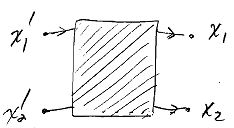
\includegraphics[width=0.3\textwidth]{2-8-1.png}
\end{center}

As we did in the single-particle Green's function, $\nu$-numbers of interaction Hamiltonians can be divided into $n$-numbers of those interaction Hamiltonian which are connected to these external lines. And $(\nu-n)$-numbers of the interaction Hamiltonians which are disconnected from these external lines.

The temporal arguments of the former group of interaction Hamiltonian and those of the latter are nothing to do with each other.

As such, we can rewrite this as
\[ \begin{split} &(i)^2\tilde{G}^{(\nu)}_{\alpha,\beta;\gamma,\delta}(x_1,x_2;x_1^{'},x_2^{'})\\
 =& \left( \frac{-i}{\hbar} \right)^\nu \frac{1}{\nu!} \int_{-\infty}^{+\infty}\mathrm{d}t_1 \ldots \int_{-\infty}^{+\infty}\mathrm{d}t_\nu \\
&\times \langle \Phi_0 | \Gamma[\hat{H}_1(t_1)\ldots\hat{H}_1(t_\nu)\hat{\psi}_\alpha(x_1) \hat{\psi}_\beta(x_2) \hat{\psi}_\gamma^\dagger(x_2^{'}) \hat{\psi}_\delta^\dagger(x_1^{'})]|\Phi_0\rangle\\
=& \sum_{n=0}^{\nu}\left( \frac{-i}{\hbar} \right)^\nu \frac{1}{\nu!}\cdot\frac{\nu!}{n!(\nu-n)!}\\
&\times\int_{-\infty}^{+\infty}\mathrm{d}t_1 \ldots \int_{-\infty}^{+\infty}\mathrm{d}t_n
\langle \Phi_0 | \Gamma[\hat{H}_1(t_1)\ldots\hat{H}_1(t_n)\hat{\psi}_\alpha(x_1) \hat{\psi}_\beta(x_2) \hat{\psi}_\gamma^\dagger(x_2^{'}) \hat{\psi}_\delta^\dagger(x_1^{'})]|\Phi_0\rangle\\
&\times\int_{-\infty}^{+\infty}\mathrm{d}t_1 \ldots \int_{-\infty}^{+\infty}\mathrm{d}t_{\nu-n}
\langle \Phi_0 | \Gamma[\hat{H}_1(t_1)\ldots\hat{H}_1(t_{\nu-n})]|\Phi_0\rangle
\end{split} \]

Here we put this factor, because the numbers of ways of dividing $\nu$-number of interaction Hamiltonians into $n$-numbers of interaction Hamiltonians and $(\nu-n)$-numbers of interaction Hamiltonians.

When we take the summation over $\nu$, the denominator can be decomposed into two part:
\[ \begin{split} &(i)^2\sum_{\nu=0}^{+\infty}\tilde{G}^{(\nu)}_{\alpha,\beta;\gamma,\delta}(x_1,x_2;x_1^{'},x_2^{'}) \\
=& \sum_{n=0}^{+\infty}\left( \frac{-i}{\hbar} \right)^n \frac{1}{n!} \int_{-\infty}^{+\infty}\mathrm{d}t_1 \ldots \int_{-\infty}^{+\infty}\mathrm{d}t_n\\&\times
\langle \Phi_0 | \Gamma[\hat{H}_1(t_1)\ldots\hat{H}_1(t_n)\hat{\psi}_\alpha(x_1) \hat{\psi}_\beta(x_2) \hat{\psi}_\gamma^\dagger(x_2^{'}) \hat{\psi}_\delta^\dagger(x_1^{'})]|\Phi_0\rangle\\
&\times\sum_{m=0}^{+\infty}\left( \frac{-i}{\hbar} \right)^m \frac{1}{m!} \int_{-\infty}^{+\infty}\mathrm{d}t_1 \ldots \int_{-\infty}^{+\infty}\mathrm{d}t_m
\langle \Phi_0 | \Gamma[\hat{H}_1(t_1)\ldots\hat{H}_1(t_m)]|\Phi_0\rangle
\end{split} \]

where the latter part can be set off by the denominator.

As a result, the two-particle Green's function can be also given by the sum of all connected Feynman diagrams.
\[ \begin{split} &(i)^2 G_{\alpha,\beta;\gamma,\delta}(x_1,x_2;x_1^{'},x_2^{'}) \\
=& \sum_{\nu=0}^{+\infty}\left( \frac{-i}{\hbar} \right)^\nu \frac{1}{\nu!} \int_{-\infty}^{+\infty}\mathrm{d}t_1 \ldots \int_{-\infty}^{+\infty}\mathrm{d}t_\nu\\&\times
\langle \Phi_0 | \Gamma[\hat{H}_1(t_1)\ldots\hat{H}_1(t_\nu) \psi_\alpha(x_1) \psi_\beta(x_2) \psi_\gamma^\dagger(x_2^{'}) \psi_\delta^\dagger(x_1^{'})]|\Phi_0\rangle
\end{split} \]

Feynman's rule for the two particle Green's function can be readily derived as a generalization of the Feynman's rule for the single-particle Green's function.

For the $n$-th order contribution to the two-particle Green's function $G_{\alpha,\beta;\gamma,\delta}(x_1,x_2;x_2^{'},x_1^{'})$:
\begin{enumerate}[(a)]
\item Draw \underline{all topologically distict} connected diagrams with $n$ interaction lines, $\nu$ and $(2n+2)$ Green's function $G^0$.
\item Label each vertex with a four dimensional space-time coordinate $x_i$.
\item Each solid line represents a Green's function $G^0_{\alpha,\beta}(x,y)$, running from $y$ to $x$.
\item Each wavy line represents an interaction
\[U_{\lambda,\lambda^{'};\mu,\mu^{'}}(x,y) = V_{\lambda,\lambda^{'};\mu,\mu^{'}}(\mathbf{x},\mathbf{y}) \delta(t_x-t_y)\]
\item Integrate all internal variables over space \& time.
\item Take the sum over all the spin indices along each fermion line.

Now that we have four external variables associated with these four fermion field operators.

\begin{center} \label{Fig2.8.2}
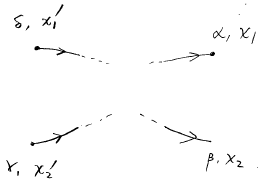
\includegraphics[width=0.3\textwidth]{2-8-2.png}
\end{center}

Two fermion lines which start from these two points should be terminated to either $\alpha$, $x_1$ or $\beta$, $x_2$.

We have two way of connecting these two creation fields with these two annihilation fields.

One is to connect $(\delta,x_1^{'})$ with $(\alpha,x_1)$ and $(\gamma,x_2^{'})$ with $(\beta,x_2)$.

\begin{center} \label{Fig2.8.3}
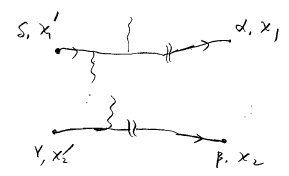
\includegraphics[width=0.3\textwidth]{2-8-3.png}
\end{center}

The other is to connect $(\delta,x_1^{'})$ with $(\beta,x_2)$ and $(\gamma,x_2^{'})$ with $(\alpha,x_1)$

\begin{center} \label{Fig2.8.4}
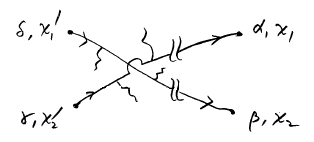
\includegraphics[width=0.3\textwidth]{2-8-4.png}
\end{center}

\item We affix a sign factor $(-1)^F$ to the former type of Feynman diagram where ``$F$" is the number of closed fermion loops in the diagram, while we affix a sign factor $(-1)^{F+1}$ to the ladder type of Feynman diagram.

* This additional $(-1)$ factor simply comes from the $(-1)$ factor which we get when exchanging these two creation operators.

The $n$-th order term has an explicit numerical factor $\left( \frac{-i}{\hbar} \right)^n$, while the $(2n+2)$ contractions of field operators contribute an additional factor $(i)^{2n+2}$.

On top of this, we have $(-i)^2$ factor, in the definition of the two-particle Green's function.
\item Thus, to compute $G_{\alpha,\beta;\gamma,\delta}(x_1,x_2;x_2^{'},x_1^{'})$, we assign a factor $(-i)^2\cdot\left( \frac{-i}{\hbar} \right)^n(i)^{2n+2} = \left( \frac{i}{\hbar} \right)^n$ to every $n$-th order term.

\item Finally, for a Green's function with equal time variables must be interpreted as $G_{\alpha,\beta}^0 (\mathbf{x},t;\mathbf{x}^{'},t+0)$.
\end{enumerate}

\begin{center}--------------------------\end{center}

These are all about the Feynman's rule for two-particle Green's function in the real space representation.

With this Feynman's rule in mind, let us go back to the density-density correlation function:
\[i D(x,x^{'}) = \frac{\langle \Psi_0|\Gamma[\tilde{n}_H(x)\tilde{n}_H(x^{'})]|\Psi_0\rangle} {\langle \Psi_0|\Psi_0 \rangle}\]

where we omit the fictitious mechanical parameter $\lambda$.

The r.h.s. can be calculated as follows:
\[ \begin{split} i D(x,x^{'})
=&\frac{1}{\langle \Psi_0 | \Psi_0 \rangle}\left\{
\begin{split} \langle \Psi_0|\Gamma[&\{\sum_\alpha \psi_{H,\alpha}^\dagger(x)\psi_{H,\alpha}(x)-\langle n_H (x) \rangle\}\\
&\{\sum_\beta \psi_{H,\beta}^\dagger(x^{'}) \psi_{H,\beta}(x^{'})-\langle n_H (x^{'}) \rangle\}]|\Psi_0 \rangle
 \end{split} \right\}\\
=&\frac{1}{\langle \Psi_0 | \Psi_0 \rangle}\\
&\sum_{\alpha,\beta} \langle \Psi_0 | \Gamma\{\psi_{H,\alpha}^\dagger(x)\psi_{H,\alpha}(x)\psi_{H,\beta}^\dagger(x^{'})\psi_{H,\beta}(x^{'})\}|\Psi_0 \rangle\\
&-\langle n_H(x) \rangle \langle n_H(x^{'}) \rangle\\
=& - \left( \sum_{\alpha,\beta} G_{\alpha,\beta;\beta,\alpha}(x,x^{'};x,x^{'}) - \sum_{\alpha} G_{\alpha,\alpha}(x,x) \sum_{\beta}G_{\beta,\beta}(x^{'},x^{'}) \right)
 \end{split}\]

Now both the two-particle Green's function here and the one-particle Green's function here are given by the sum of connected Feynman diagrams.

Especially, two-particle Green's function contain those Feynman diagrams in which the external line from $x,\alpha$ to $x,\alpha$ and that from $x^{'},\beta$ to $x^{'},\beta$ are disconnected.

\begin{center} \label{Fig2.8.5}
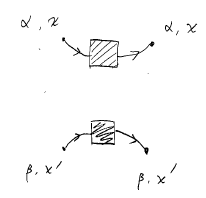
\includegraphics[width=0.3\textwidth]{2-8-5.png}
\end{center}

Connected Feynman diagrams to $G_{\alpha,\beta;\beta,\alpha}(x,x^{'};x,x^{'})$, in which an external line from $(\alpha,x)$ to $(\alpha,x)$ and that from $(\beta,x^{'})$ to $(\beta,x^{'})$ are disconnected.

\begin{center}--------------------------\end{center}

Since each of these two are described by single particle Green's functions $G_{\alpha,\alpha}(x,x)$ and $G_{\beta,\beta}(x^{'},x^{'})$ respectively, such Feynman diagrams are completely cancelled by this second term.

Such a cancellation becomes possible, because any $n$-th order term in this class of diagrams are accompanied by $\left(\frac{i}{\hbar}\right)^n (-1)^F$ where $F$ denotes the number of fermion loop.

Such a factor can be always decomposed into two part:
\[ \left(\frac{i}{\hbar}\right)^n (-1)^F=\left(\frac{i}{\hbar}\right)^{n_1} (-1)^{F_1}\cdot\left(\frac{i}{\hbar}\right)^{n_2} (-1)^{F_2} \]

each of which can be ascribed to these two part respectively.

Thus.
\[\begin{split}
-i D(x,x^{'})=& \sum_{\alpha,\beta} G_{\alpha,\beta;\beta,\alpha}(x,x^{'};x,x^{'}) - \sum_{\alpha}G_{\alpha,\alpha}(x,x)\cdot\sum_{\beta}G_{\beta,\beta}(x^{'},x^{'})\\
=& \sum_{\alpha,\beta}G_{\alpha,\beta;\beta,\alpha}^{(C)}(x,x^{'};x^{'},x)
\end{split}\]

where this superscript ``$(C)$" means that the fermion field at $(\alpha,x)$ and the fermion field at $(\beta,x^{'})$ is always connected in these Feynman diagrams.

Examples of such Feynman diagrams include,
\begin{center} \label{Fig2.8.6}
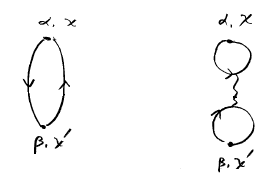
\includegraphics[width=0.3\textwidth]{2-8-6.png}
\end{center}

Here, I put together two fermion fields whose arguments are same.

As in eq.(\ref{Eqs2.8.3}), to obtain the ground state energy, we need the density-density correlation function as a function of $\lambda$, where $\lambda$ denotes a mechanical(fictitions) parameter we put in front of the interaction potential.

When this $\lambda$ is taken to be zero, we don't have any interaction potential. In such a case, we only have two way of contracting the fermion fields \underline{here}.
\[\begin{split}
-i D^{\lambda=0}(x,x^{'})=& \sum_{\alpha,\beta} G^{\lambda=0}_{\alpha,\beta;\beta,\alpha}(x,x^{'};x,x^{'}) - \sum_{\alpha}G^{\lambda=0}_{\alpha,\alpha}(x,x)\cdot\sum_{\beta}G^{\lambda=0}_{\beta,\beta}(x^{'},x^{'})
\end{split}\]

One is {\label{Fig2.8.7} 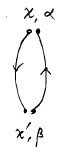
\includegraphics[width=0.05\textwidth]{2-8-7.png}} and the other is {\label{Fig2.8.8} 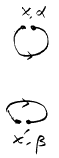
\includegraphics[width=0.05\textwidth]{2-8-8.png}}.

The latter one is cancelled by the 2nd term($\sum_{\beta} G^{\lambda=0}_{\beta,\beta}(x^{'},x^{'})$), so that the density-density correlation function is given by the former one.

Following the Feynman's rule described so far, the analytic expression for the former one is given as follows:
\[\begin{split}-i D^{\lambda=0}(x,x^{'})=&G^{\lambda=0,(C)}_{\alpha,\beta;\beta,\alpha}(x,x^{'};x,x^{'})\\
=& \underline{(-)} G^0_{\beta,\alpha}(x^{'},x) G^0_{\alpha,\beta}(x,x^{'})\end{split}\]

where this underlined $(-)$ sign comes from the interchange between these two fields.

\[D^{\lambda=0}(x,x^{'})=-i G^0_{\alpha,\beta}(x,x^{'}) G^0_{\beta,\alpha}(x^{'},x) \equiv \hbar \Pi^0(x,x^{'})\]

where we call this as a bare polarization part.

Similarly, we can define polarization part as the density-density correlation function.
\begin{equation*} \label{Eqs2.8.4'} \tag{2.8.4'}
D(x,x^{'}) \equiv \hbar \Pi(x,x^{'})
\end{equation*}

(or $D^{\lambda}(x,x^{'}) \equiv \hbar \Pi^{\lambda}(x,x^{'})$ )

Since our system is spatially and temporally homogeneous, the correlation function between two points depends only on their relative distance:
\[D^{\lambda}(x,x^{'}) = D^{\lambda}(\mathbf{x}-\mathbf{x}^{'},t-t^{'})\]

so that we can introduce its Fourier series.
\[=\int \frac{\mathrm{d}\mathbf{q}}{(2\pi)^3}\int \frac{\mathrm{d} \omega}{2\pi} \mathrm{e}^{i \mathbf{q}(\mathbf{x}-\mathbf{x}^{'})-i \omega(t-t^{'})}D^{\lambda}(\mathbf{q},\omega)\]

In the momentum representation, the bare polarization part is given as follows.
\[ \hbar \Pi^0(\mathbf{q},\omega) = -i \int \frac{\mathrm{d}\mathbf{k}}{(2\pi)^3} \int \frac{\mathrm{d}\epsilon}{2\pi} G^0_{\alpha,\beta}(\mathbf{k}+\mathbf{q},\epsilon+\omega)G^0_{\beta,\alpha}(\mathbf{k},\epsilon) \]

and: the corresponding Feynman diagram can be described like this
\begin{center} \label{Fig2.8.9}
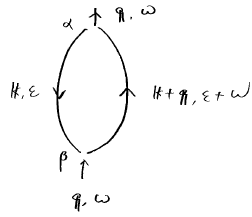
\includegraphics[width=0.3\textwidth]{2-8-9.png}
\end{center}

Similarly, Feynman diagrams for the full polarization part can be schematically described as follows:
\begin{center} \label{Fig2.8.10}
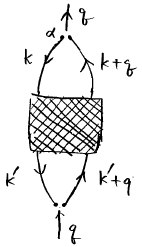
\includegraphics[width=0.15\textwidth]{2-8-10.png}
\end{center}

where $k$, $k^{'}$, $q$ here are all four-dimensional momentum vector.

This shadow region contains all possible Feynman diagrams which connect the upper part \& the lower part.

Such diagrams can be generally classified into proper part and inproper part, in the same way as we did for the self-energy.

The proper part is a polarization part that \textbf{cannot} be separated into two part by cutting a single interaction line. While the improper part is a polarization part that \textbf{can} be divided into the upper part and lower part by cutting a single interaction line.

For example, this is a proper polarization part, while this is improper, because we can cut this into two polarization part by removing this interaction line.
\begin{center} \label{Fig2.8.11}
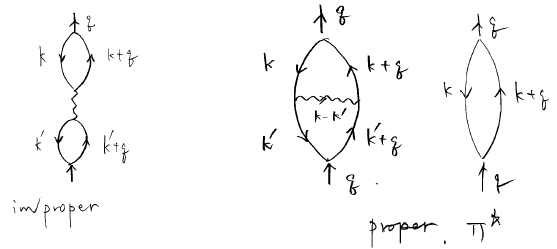
\includegraphics[width=0.6\textwidth]{2-8-11.png}
\end{center}

\begin{center}--------------------------\end{center}

Then, in the same way as we did for the Dyson equation for self-energy, we can also derive the Dyson equation for the polarization part:

\begin{itemize}
\item Firstly, the full polarization part consist of a sum of all possible repetitions of the proper polarization part.
\begin{center} \label{Fig2.8.12}
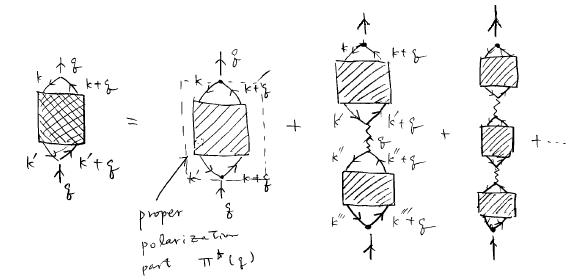
\includegraphics[width=0.8\textwidth]{2-8-12.png}
\end{center}

where this part denotes the proper polarization part, while this wavy line is for interaction potential.

\item This description becomes possible, especially because any $n$-th order Feynman diagram is accompanied by $\left( \frac{i}{\hbar} \right)^n \cdot (-1)^{F^{'}}$, where $F^{'}$ stands for the number of fermion loop.

\item As is clear from this repetitive structure, this can be rewritten into a self-consistent equation:
\begin{center} \label{Fig2.8.13}
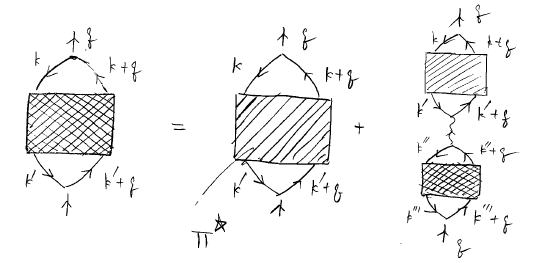
\includegraphics[width=0.8\textwidth]{2-8-13.png}
\end{center}

where this singly shaded one is a collection of all possible proper polarization part.

while this doubly daded one denote a collection of all possible polarization part.
\end{itemize}

This equation is called as Dyson's equation for polarization part and its analytic expression is given like this:
\[(-i \hbar)\Pi(q) = (-i \hbar)\Pi^{\bigstar}(q)+(-i \hbar)\Pi^{\bigstar}(q) \cdot \frac{i}{\hbar} V(q) (-i\hbar)\Pi(q)\]

Here $V(q)$ stands for the Fourier transform of the interaction potential, which corresponds to this wavy line.

As I mentioned already, we assumed spin-independent interaction potential.
\[V_{\lambda,\lambda^{'};\mu,\mu^{'}}(\mathbf{x},\mathbf{x}^{'}) = V(\mathbf{x}-\mathbf{x}^{'}) \delta_{\lambda\lambda^{'}}\delta_{\mu\mu^{'}}\]

with $V(\mathbf{q})=\int \mathrm{d}^3 \mathbf{x} \mathrm{e}^{-i \mathbf{k} \mathbf{x}} V(\mathbf{x})$.

so that the product between $\Pi_0(q)$ and $V(\mathbf{q})$ and $V(\mathbf{q})$ and $\Pi(q)$ reduces to a single scalar product.

This interaction potential is accompanied by $\left( \frac{i}{\hbar} \right)$, which is this. Remember also that both $\Pi_0$ and $\Pi$ are always accompanied by factor $(-i \hbar)$ here.
This factor($-i \hbar$) comes from our definition of polarization part:\footnote{see eq.(\ref{Eqs2.8.4})}
\[-i \hbar \Pi(x,x^{'})\equiv -i D(x,x^{'}) \equiv (-i)^2 \frac{\langle \Psi_0 | \Gamma[\tilde{n}_H(x)\tilde{n}_H(x^{'})]|\Psi_0\rangle}{\langle\Psi_0|\Psi_0\rangle}\]

Namely, I put this factor in front of the polarization part, in order to make this corresponding r.h.s. to be consistent with definition of two-particle Green's function, for which we can apply Feynman's rule.

With these factors in mind, one can see that this equation can be simplified into this form:
\begin{equation} \label{Eqs2.8.5}
\Pi(q) = \Pi^{\bigstar}(q)+\Pi^{\bigstar}(q) V(q) \Pi(q)
\end{equation}

which can be solved exactly as
\begin{equation*} \label{Eqs2.8.5'} \tag{2.8.5'} \Pi(q) = \frac{\Pi^{\bigstar}(q)}{1-\Pi^{\bigstar}(q) V(q)} \end{equation*}

Then, the density-density correlation function is given as follows:
\begin{equation} \label{Eqs2.8.6}
D^{\lambda}(x,x^{'}) = \hbar \Pi^{\lambda}(x,x^{'}) = \frac{\hbar \Pi^{\bigstar,\lambda}(q)}{1-\lambda\Pi^{\bigstar,\lambda}(q) V(q)} = \frac{\hbar \Pi^{\bigstar,\lambda}(q)}{K^{\lambda}(q)}
\end{equation}

Here, I put $\lambda$ in order to make explicit the $\lambda$-dependence of the correlation function.

substituting this back into eq.(\ref{Eqs2.8.3}), we finally obtain
\begin{eqnarray}
E_{corr} =& \frac{i}{2} V \int_0^1 \mathrm{d}\lambda \cdot \lambda^{-1} \int \frac{\mathrm{d}^4 q}{(2\pi)^4} \lambda V(q) [D^{\lambda}(q)-D^0(q)]\nonumber\\
=& \frac{i}{2} \hbar V \int_0^1 \mathrm{d}\lambda \cdot \lambda^{-1} \int \frac{\mathrm{d}^4 q}{(2\pi)^4} \left[ \frac{\lambda V(q)\Pi^{\bigstar,\lambda}(q)}{1-\lambda V(q)\Pi^{\bigstar,\lambda}(q)} - \lambda V(q)\Pi^0(q) \right] \label{Eqs2.8.7}\\
=& \frac{i}{2} \hbar V \int_0^1 \mathrm{d}\lambda \cdot \lambda^{-1} \int \frac{\mathrm{d}^4 q}{(2\pi)^4} \left[ -1 + \frac{1}{1-\lambda V(q)\Pi^{\bigstar,\lambda}(q)} - \lambda V(q)\Pi^0(q) \right] \nonumber\\
=&\frac{i}{2} \hbar V \int_0^1 \mathrm{d}\lambda \cdot \lambda^{-1} \int \frac{\mathrm{d}^4 q}{(2\pi)^4} \left[ \left[ K^{\lambda}(q) \right]^{-1} - 1 - \lambda V(q)\Pi^0(q) \right] \label{Eqs2.8.8}
\end{eqnarray}

where $V$ here denote the total volume of the system.

Eq.(\ref{Eqs2.8.8}) can be applied to any homogeneous system with spin-independent interaction.

In the following, however, we specialize to a degenerate electron gas with long-range Coulomb interaction, whose Hamiltonian is already defined in eq.(\ref{eq1.8.14}).

As I have already explained there, the uniform positive background precisely cancels the $\mathbf{q}=0$ term in the interaction potential $V(\mathbf{q})$, so that $V(\mathbf{q}=0)$ vanishes.

To understand the structure of eq.(\ref{Eqs2.8.8}), let us expand $\left[ \ldots \right]$ in $\lambda$(or interaction potential):
\footnote{\begin{center} \label{Fig2.8.14}
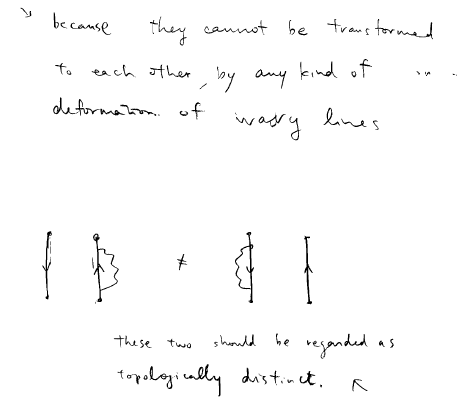
\includegraphics[width=0.6\textwidth]{2-8-14.png}
\end{center}}

\[[\ldots] = \frac{\lambda V(q)\Pi^{\bigstar,\lambda}(q)}{1-\lambda V(q)\Pi^{\bigstar,\lambda}(q)} - \lambda V(q)\Pi^0(q)\]

Generally, the proper polarization part depends on $\lambda$ in a non-trivial manner.

But, we can expand $\Pi^{\bigstar,\lambda}$ in the powers of $\lambda$:
\[ \Pi^{\bigstar,\lambda}(q) = \Pi^{\bigstar}_0(q) + \lambda\Pi^{\bigstar}_1(q)+\lambda^2 \Pi^{\bigstar}_2(q) + \ldots \]

where
\begin{itemize}
\item \[\Pi_0^\bigstar(q)= 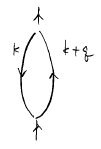
\includegraphics[width=0.1\textwidth]{2-8-15.png}\quad(\equiv \Pi_0(q))\]

\item \[\Pi_1^\bigstar(q) = 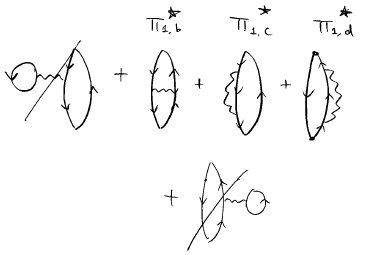
\includegraphics[width=0.4\textwidth]{2-8-16.png} \]

The 1st term and last term vanish because $V(\mathbf{q}=0)=0$.

\item \[\Pi_2^\bigstar(q) = \ldots\]
\end{itemize}

With this expansion in mind, we can expand this in powers of $\lambda$ as:
\[ [\ldots] = \lambda V(q) \Pi_0^\bigstar(q) + \lambda^2 V(q) \Pi_1^\bigstar(q) + \lambda^2 V(q) \Pi_0^\bigstar(q) V(q) \Pi_0^\bigstar(q) + \ldots - \lambda V(q) \Pi^0(q)\]

Now $\Pi_0^\bigstar = \Pi^0$, so that this starts from 2nd order in $\lambda$.
\[ [\ldots] = \lambda^2 V(q) \Pi_1^\bigstar(q) + \lambda^2 \left( V(q) \Pi^0 (q) \right)^2 \]

Correspondingly, we have the expansion of ground state energy as
\[E_{corr} = E_2^r + E_2^b + E_2^c + E_2^d+\ldots\]

where
\[\begin{split}E_2^r =& \frac{1}{2}i V \hbar \int_0^1 \mathrm{d} \lambda \cdot \lambda^{-1} \int \frac{\mathrm{d}^4 q}{(2\pi)^4} \left[ \lambda V_0(q)\Pi^0(q) \right]^2\\
E_2^{b,c,d} =& \frac{1}{2}i V \hbar \int_0^1 \mathrm{d} \lambda \cdot \lambda^{-1} \int \frac{\mathrm{d}^4 q}{(2\pi)^4} \left[ \lambda V_0(q)\Pi^\bigstar_{1,b,c,d}(q) \right]
 \end{split}\]

where we named these 3 as $\Pi_{1,b}$, $\Pi_{1,c}$, $\Pi_{1,d}$ respectively.

One can explicitly show that the correlation energy due to these proper polarization parts are finite.

On the one hand, the correlation energy dut to this improper polartization part contain the logarithmic divergence of the $q$-integral, which we will see later.

This divergence comes from the singular behaviour of the Coulomb potential $V(q)\equiv \frac{4\pi e^2}{\mathbf{q}^2}$ for small $\mathbf{q}$ region. Namely, $E_2^r$ contains two $V(q)$, which gives its intergrand with $\mathbf{q}^{-4}$ behaviour.

A similar divergence also occurs in all orders in $\lambda$, because these is always a single $m$-th order term with the integrand $\left[ V(q) \Pi^0(q) \right]^m$.

\begin{center} \label{Fig2.8.17}
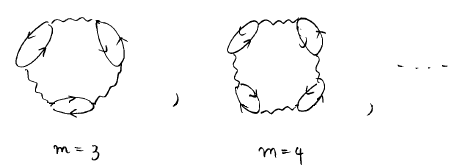
\includegraphics[width=0.6\textwidth]{2-8-17.png}
\end{center}

An idea of ``ring diagram approximation" is to sum up all these singular terms up to all order in the perturbation theory by introducting an effective interaction potential as
\[\begin{split} U_r(q) =& V(q) + V(q)\Pi^0(q) V(q) + [V(q)\Pi^0(q)]^2 V(q) + [V(q)\Pi^0(q)]^3 V(q) + \ldots \\ 
=& \frac{V(q)}{1-V(q)\Pi^0(q)}
\end{split}\]

Namely, with this effective interaciton potential, these singular terms can be summed up in all order in $\lambda$ as
\begin{equation} \label{Eqs2.8.9} \begin{split}
E_r =& \frac{1}{2}i V\hbar \int_0^1 \mathrm{d} \lambda \cdot \lambda^{-1} \int \frac{\mathrm{d}^4 q}{(2\pi)^4} \sum_{n=2}^\infty [ \lambda V_0(q) \Pi^0(q) ]^n\\
=& \frac{1}{2}i V\hbar \int_0^1 \mathrm{d} \lambda \cdot \lambda^{-1} \int \frac{\mathrm{d}^4 q}{(2\pi)^4} \frac{[\lambda V_0(q) \Pi^0(q)]^2}{1-\lambda V_0(q) \Pi^0(q)}\\
=& \frac{1}{2}i V\hbar \int_0^1 \mathrm{d} \lambda \cdot \lambda^{-1} \int \frac{\mathrm{d}^4 q}{(2\pi)^4} \lambda V_0(q) \Pi^0(q) \underline{U_r^\lambda(q)} \Pi^0(q)
\end{split}\end{equation}

where the underlined term is the effective interaction potential.

To summarize, the correlation energy of a degenerate electron gas can be given as
\[E_{corr} = E_r + E_2^b + E_2^c + E_2^d+\ldots\]

where $E_r$ is the collection of leading contributions, while $E_2^{b,c,d}$ are at most finite and less leading contribution.

$E_r$ can be schematically given by the following diagrams:
\begin{center} \label{Fig2.8.18}
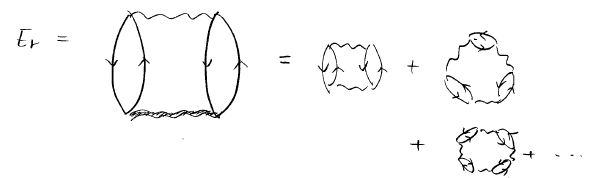
\includegraphics[width=0.6\textwidth]{2-8-18.png}
\end{center}

where the bold wavy line represents the effective interaction potential $U_r(q)$;
\begin{center} \label{Fig2.8.19}
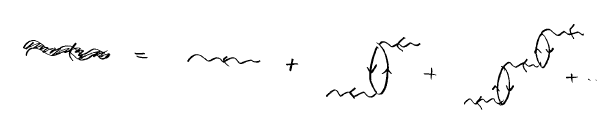
\includegraphics[width=0.6\textwidth]{2-8-19.png}
\end{center}

Taking into account only these singular diagrams is called a ``ring-diagram approximation".

Ring-diagram approximation is equivalent to employing Dyson equation with its proper polarization part being replaced by the zero-th order contribution.

Namely, when we replace $\Pi^{\bigstar,\lambda}(q)$ in eq.(\ref{Eqs2.8.7}) by its zero-th order contribution $\Pi^0(q)$, we safely have $E_r$:
\begin{equation*} \begin{split}
E_{corr} =&\frac{i}{2} \hbar V \int_0^1 \mathrm{d}\lambda \cdot \lambda^{-1} \int \frac{\mathrm{d}^4 q}{(2\pi)^4} \left[ \frac{\lambda V(q) \Pi^{\bigstar,\lambda}(q)}{1- \lambda V(q) \Pi^{\bigstar,\lambda}(q)} - \lambda V(q)\Pi^0(q) \right]\\
\approx& \frac{i}{2} \hbar V \int_0^1 \mathrm{d}\lambda \cdot \lambda^{-1} \int \frac{\mathrm{d}^4 q}{(2\pi)^4} \left[ \frac{\lambda V(q) \Pi^0(q)}{1- \lambda V(q) \Pi^0(q)} - \lambda V(q)\Pi^0(q) \right]\\
=& \frac{i}{2} \hbar V \int_0^1 \mathrm{d}\lambda \cdot \lambda^{-1} \int \frac{\mathrm{d}^4 q}{(2\pi)^4} \frac{[\lambda V(q) \Pi^0(q)]^2}{1- \lambda V(q) \Pi^0(q)}\\
=& E_r 
\end{split}\end{equation*}

Correspondingly, the effective interaction potential $U_r(q)$ can be rewritten in terms of a dielectric constant.
\begin{eqnarray}
U_r(q) = \frac{V(q)}{K_r(q)} \label{Eqs2.8.10}\\
K_r(q) = 1-V(q) \Pi^0(q) \label{Eqs2.8.11}
\end{eqnarray}

Where $K_r(q)$ can be regarded as the ring-diagram approximation to the exact dielectric constant.

We next evaluate this lowest-order proper polarization part. $\Pi_0(q)$
\begin{equation} \label{Eqs2.8.12}
\Pi_0(q) = - \frac{2i}{\hbar} \int \frac{\mathrm{d}^3 \mathbf{k}}{(2\pi)^3} \int \frac{\mathrm{d} \epsilon}{2\pi} G^0(\mathbf{k}+\mathbf{q},\epsilon+\omega) G^0(\mathbf{k},\epsilon)
\end{equation}

where this factor 2 comes from the summation over the spin index, using this
\begin{equation} \label{Eqs2.8.13}
G^0(\mathbf{k},\epsilon) = \frac{\theta(|\mathbf{k}|-k_F)}{\omega-\omega_{\mathbf{k}}+i \eta} + \frac{\theta(k_F - |\mathbf{k}|)}{\omega-\omega_{\mathbf{k}}-i \eta}
\end{equation}

we have
\[\begin{split}\Pi_0(q) =&- \frac{2i}{\hbar} \int \frac{\mathrm{d}^3 \mathbf{k}}{(2\pi)^3} \int_{-\infty}^{+\infty} \frac{\mathrm{d} \epsilon}{2\pi} \times \left\{ \frac{\theta(|\mathbf{k}+\mathbf{q}|-k_F)}{\epsilon+\omega-\omega_{\mathbf{k}+\mathbf{q}} +i \eta} + \frac{\theta(k_F - |\mathbf{k}+\mathbf{q}|)}{\epsilon + \omega - \omega_{\mathbf{k}+\mathbf{q}}-i \eta} \right\}\\
&\times \left\{ \frac{\theta(|\mathbf{k}|-k_F)}{\epsilon-\omega_{\mathbf{k}} +i \eta} + \frac{\theta(k_F - |\mathbf{k}|)}{\epsilon - \omega_{\mathbf{k}}-i \eta} \right\} \end{split}\]

Out of this integrand, we have four terms, 2 of which vanish under the integration over $\epsilon$.

Namely, product between these two and that between these two have their poles only in the lower half plane and only in the upper half plane respectively.

Such terms reduce to zero, when we close the contour in the opposite side of the half plane.

Accordingly, we end up a product between these two and that between these two.\[\begin{split}\Pi_0(q) =- \frac{2i}{\hbar} \int \frac{\mathrm{d}^3 \mathbf{k}}{(2\pi)^3} \int_{-\infty}^{+\infty} \frac{\mathrm{d} \epsilon}{2\pi} \times &\left\{  \frac{\theta(|\mathbf{k}+\mathbf{q}|-k_F)}{\epsilon+\omega-\omega_{\mathbf{k}+\mathbf{q}} +i \eta} \cdot \frac{\theta(k_F - |\mathbf{k}|)}{\epsilon - \omega_{\mathbf{k}}-i \eta} \right.\\
&\left.+ \frac{\theta(k_F - |\mathbf{k}+\mathbf{q}|)}{\epsilon + \omega - \omega_{\mathbf{k}+\mathbf{q}}-i \eta} \cdot \frac{\theta(|\mathbf{k}|-k_F)}{\epsilon-\omega_{\mathbf{k}} +i \eta} \right\} 
 \end{split}\]

\[\begin{split}=\frac{2}{\hbar} \int \frac{\mathrm{d}^3 \mathbf{k}}{(2\pi)^3}
 &\left\{  \frac{\theta(|\mathbf{k}+\mathbf{q}|-k_F)\theta(k_F - |\mathbf{k}|)}{\omega + \omega_{\mathbf{k}}- \omega_{\mathbf{k}+\mathbf{q}} +\underline{2}i \eta} - \frac{\theta(k_F - |\mathbf{k}+\mathbf{q}|) \theta(|\mathbf{k}|-k_F)}{\omega + \omega_{\mathbf{k}} - \omega_{\mathbf{k}+\mathbf{q}}-\underline{2}i \eta} \right\} 
 \end{split}\]

As for the 2nd term, we can define $\mathbf{k}^{'} = -\mathbf{k}-\mathbf{q}$, so that, $\mathbf{k}$ and $\mathbf{k} + \mathbf{q}$ are replaced by $-\mathbf{k}^{'}-\mathbf{q}$ and $-\mathbf{k}^{'}$ respectively.

Now $\omega_\mathbf{k}$ are an even function in momentum. these two can be replaced by $\mathbf{k}^{'} + \mathbf{q}$ and $\mathbf{k}^{'}$ respectively.

$\mathbf{k}^{'}$ as well as $\mathbf{k}$ are dummy index, we can replace $\mathbf{k}^{'}$ by $\mathbf{k}$.
\[=\frac{2}{\hbar} \int \frac{\mathbf{d}^3 \mathbf{k}}{(2\pi)^3}\theta(|\mathbf{k}+\mathbf{q}|-k_F)\theta(k_F - |\mathbf{k}|) \times \left\{ \frac{1}{\omega+\omega_{\mathbf{k}}- \omega_{\mathbf{k}+\mathbf{q}}+i \eta} - \frac{1}{\omega-\omega_{\mathbf{k}}+ \omega_{\mathbf{k}+\mathbf{q}}-i \eta} \right\}\]

This clearly suggests that $\Pi^0(\mathbf{q},\omega)$ is an even function of $\omega$.
\begin{equation} \label{Eqs2.8.14} \Pi^0(\mathbf{q},\omega) = \Pi^0(\mathbf{q},-\omega)\end{equation}

so that we have only to study $\Pi^0(\mathbf{q},\omega)$ for positive $\omega$
\begin{center}-----------------------\end{center}

Let us begin with the real part of $\Pi^0(\mathbf{q},\omega)$:
\footnote{This ``$\mathscr{P}$" stands for the principal integral(value).}
\begin{equation} \label{Eqs2.8.15} \begin{split}
\text{Re} \Pi^0(\mathbf{q},\omega) =& \frac{2}{\hbar} \int \frac{\mathrm{d}^3 \mathbf{k}}{(2\pi)^3} \theta(|\mathbf{k}+\mathbf{q}|-k_F)\theta(k_F - |\mathbf{k}|)\\
& \times \left\{ \frac{\mathscr{P}}{\omega+\omega_{\mathbf{k}}- \omega_{\mathbf{k}+\mathbf{q}}} - \frac{\mathscr{P}}{\omega-\omega_{\mathbf{k}}+ \omega_{\mathbf{k}+\mathbf{q}}} \right\}
\end{split}\end{equation}
\begin{equation} \label{Eqs2.8.16} \begin{split}
\text{Im} \Pi^0(\mathbf{q},\omega) =& -\frac{1}{\hbar} \int \frac{\mathrm{d}^3 \mathbf{k}}{(2\pi)^3} \theta(|\mathbf{k}+\mathbf{q}|-k_F)\theta(k_F - |\mathbf{k}|) \\
&\times \left\{ \delta(\omega+\omega_{\mathbf{k}}- \omega_{\mathbf{k}+\mathbf{q}}) + \delta(\omega-\omega_{\mathbf{k}}+ \omega_{\mathbf{k}+\mathbf{q}}) \right\}
\end{split}\end{equation}

By replacing $\theta(|\mathbf{k}+\mathbf{q}|-k_F)$ by $1-\theta(k_F - |\mathbf{k}+\mathbf{q}|)$, we have
\[ \text{Re} \Pi^0(\mathbf{q},\omega) = \frac{2}{\hbar} \mathscr{P} \int \frac{\mathrm{d}^3 \mathbf{k}}{(2\pi)^3} \left( 1-\theta(k_F-|\mathbf{k}+\mathbf{q}|)\right)\theta(k_F - |\mathbf{k}|) \times \left\{ \frac{1}{\omega+\omega_{\mathbf{k}}- \omega_{\mathbf{k}+\mathbf{q}}} - \frac{1}{\omega-\omega_{\mathbf{k}}+ \omega_{\mathbf{k}+\mathbf{q}}} \right\}
\]

This part vanishes under the $\mathbf{k}$-integral.

One can see this by introducing again $\mathbf{k}^{'}=-\mathbf{k}-\mathbf{q}$.

\[ \text{Re} \Pi^0(\mathbf{q},\omega) = \frac{2}{\hbar} \mathscr{P} \int \frac{\mathrm{d}^3 \mathbf{k}}{(2\pi)^3} \theta(k_F - |\mathbf{k}|) \times \left\{ \frac{1}{\omega+\omega_{\mathbf{k}}- \omega_{\mathbf{k}+\mathbf{q}}} - \frac{1}{\omega-\omega_{\mathbf{k}}+ \omega_{\mathbf{k}+\mathbf{q}}} \right\}
\]

$\omega_{\mathbf{k}}$ denotes the kinetic energy of electron gas;
\[ \omega_{\mathbf{k}} = \frac{\epsilon_{\mathbf{k}}}{\hbar} = \frac{\hbar \mathbf{k}^2}{2m} \]

so that we have
\begin{equation} \label{Eqs2.8.17} \begin{split}
\omega_{\mathbf{k}+\mathbf{q}} - \omega_{\mathbf{k}} =& \frac{\hbar}{2m}\left( (\mathbf{k}+\mathbf{q})^2-\mathbf{k}^2 \right)\\
=& \frac{\hbar}{2m}\left( 2 \mathbf{k} \cdot \mathbf{q} + \mathbf{q}^2 \right)\\
=& \frac{\hbar}{m} \left( \mathbf{k}\cdot \mathbf{q} + \frac{\mathbf{q}^2}{2} \right)
\end{split}\end{equation}

using this, the real part is given by
\[ \text{Re} \Pi^0(\mathbf{q},\omega) = \frac{2}{\hbar} \mathscr{P} \int \frac{\mathrm{d}^3 \mathbf{k}}{(2\pi)^3} \theta(k_F - |\mathbf{k}|) \times \left\{ \frac{1}{\omega-\frac{\hbar}{m}(\mathbf{q}\cdot\mathbf{k}+\frac{\mathbf{q}^2}{2})} - \frac{1}{\omega+\frac{\hbar}{m}(\mathbf{q}\cdot\mathbf{k}+\frac{\mathbf{q}^2}{2})} \right\}
\]

By making $\omega$ to be dimensionless variable and measuring all wave vectors in the unit of $k_F$;
\begin{equation} \label{Eqs2.8.18}
\nu = \frac{m}{\hbar k_F^2} \omega \qquad
\left( \begin{split} \mathbf{q}_{old} =& k_F \mathbf{q}_{new}\\
\mathbf{k}_{old} =& k_F \mathbf{k}_{new}  \end{split}\right)
\end{equation}

we have
\[ \begin{split} &\text{Re} \Pi^0_{old}(k_F\mathbf{q},\frac{\hbar k_F^2}{m}\nu) \equiv \text{Re} \Pi^0_{new}(\mathbf{q},\nu) \\
=& \frac{2 m k_F}{\hbar^2} \mathscr{P} \int \frac{\mathrm{d}^3 \mathbf{k}}{(2\pi)^3} \theta(1 - |\mathbf{k}|) \times \left\{ \frac{1}{\nu-(\mathbf{q}\cdot\mathbf{k} + \frac{\mathbf{q}^2}{2})} - \frac{1}{\nu-(-\mathbf{q}\cdot\mathbf{k}-\frac{\mathbf{q}^2}{2})} \right\}
\end{split}\]

\begin{equation} \label{Eqs2.8.19} \begin{split} \text{Re} \Pi^0(\mathbf{q},\nu)
= \frac{2 m k_F}{\hbar^2} \int_0^1 k^2 \cdot \mathrm{d} k \int_{-1}^{1} \mathrm{d} t \times \left\{ \frac{\mathscr{P}}{\nu-\underline{(q k t + \frac{q^2}{2})}} - \frac{\mathscr{P}}{\nu-(-q k t-\frac{q^2}{2})} \right\}
\end{split}\end{equation}

Since these integrals are Cauchy principal integral, we need to pay attention to those possibilities of these denominators being zero.

To clarify these possibilities, notice that this quantity(the underlined part) is bounded like this:
\[ -q+\frac{q^2}{2} \leq qkt + \frac{q^2}{2} \leq q + \frac{q^2}{2}  \]

while this quantity is bounded by this form
\[ -q-\frac{q^2}{2} \leq -qkt - \frac{q^2}{2} \leq q - \frac{q^2}{2}\]

As such, depending on $\nu$ and $q$, we have following five cases:
\begin{enumerate}[(i)]
\item $\nu > \frac{q^2}{2}+q > \frac{q^2}{2}-q, -\frac{q^2}{2}+q > -\frac{q^2}{2}-q$
\item $\frac{q^2}{2}+q>\nu > \frac{q^2}{2}-q, -\frac{q^2}{2}+q > -\frac{q^2}{2}-q$
\item $\frac{q^2}{2}+q > max(\frac{q^2}{2}-q,-\frac{q^2}{2}+q) > \nu > min(\frac{q^2}{2}-q,-\frac{q^2}{2}+q) > -\frac{q^2}{2}-q$
\item $\frac{q^2}{2} + q > \frac{q^2}{2}-q, -\frac{q^2}{2}+q>\nu>-\frac{q^2}{2}-q$
\item $\frac{q^2}{2}+q > \frac{q^2}{2}-q, -\frac{q^2}{2}+q > -\frac{q^2}{2}-q > \nu$
\end{enumerate}

In the case of (i), these are no possibilities of these denominators being zero, so that we can freely integrate this:

\[\text{Re} \Pi^0(\mathbf{q},\nu)
= -\frac{2 m k_F}{\hbar^2} \frac{1}{q} \int_0^1 k \cdot \mathrm{d} k \times \left\{ 
\left[ \log(\nu-q k t-\frac{q^2}{2}) \right]_{t=-1}^{t=+1} - \left[ \log(\nu+q k t+\frac{q^2}{2}) \right]_{t=-1}^{t=+1}
 \right\}\]

we obtain
\footnote{Using
\[ \int x \log(\beta-\alpha x) \mathrm{d}x = \frac{x^2}{2} \log(\beta - \alpha x) - \frac{\beta^2}{2 \alpha^2} \log(\beta - \alpha x) - \frac{x^2}{4}- \frac{\beta}{2\alpha}x \]}

\[ \begin{split}\text{Re} \Pi^0(\mathbf{q},\nu)
= \frac{2 m k_F}{\hbar^2} \frac{1}{4\pi^2} \times&\left\{ -1 + \frac{1}{2q}\left( 1-(\frac{\nu}{q}-\frac{q}{2})^2 \right) \log\left[ \frac{\nu-\frac{q^2}{2}+q}{\nu-\frac{q^2}{2}-q} \right] \right. \\
&\left. -\frac{1}{2q}\left( 1-(\frac{\nu}{q}+\frac{q}{2})^2 \right) \log\left[ \frac{\nu+\frac{q^2}{2}+q}{\nu+\frac{q^2}{2}-q} \right] \right\}
\end{split}\]

As for other cases, we can do a similar integral, from which we obtain.
\begin{equation} \label{Eqs2.8.20}
\begin{split}\text{Re} \Pi^0(\mathbf{q},\nu)
= \frac{2 m k_F}{\hbar^2} \frac{1}{4\pi^2} \times&\left\{ -1 + \frac{1}{2q}\left( 1-(\frac{\nu}{q}-\frac{q}{2})^2 \right) \log\left[ \frac{|\nu-\frac{q^2}{2}+q|}{|\nu-\frac{q^2}{2}-q|} \right] \right. \\
&\left. -\frac{1}{2q}\left( 1-(\frac{\nu}{q}+\frac{q}{2})^2 \right) \log\left[ \frac{|\nu+\frac{q^2}{2}+q|}{|\nu+\frac{q^2}{2}-q|} \right] \right\}
\end{split}
\end{equation}

for any cases.

Let us next calculate the imginary part of $\Pi^0(\mathbf{q},\omega)$.
\begin{equation*} \tag{2.8.16} \begin{split}
\text{Im} \Pi^0(\mathbf{q},\omega) =& -\frac{1}{\hbar} \int \frac{\mathrm{d}^3 \mathbf{k}}{(2\pi)^3} \theta(|\mathbf{k}+\mathbf{q}|-k_F)\theta(k_F - |\mathbf{k}|)\\
& \times \left\{ \delta(\omega+\omega_{\mathbf{k}}- \omega_{\mathbf{k}+\mathbf{q}}) + \delta(\omega-\omega_{\mathbf{k}}+ \omega_{\mathbf{k}+\mathbf{q}}) \right\}
\end{split}\end{equation*}

Since $\Pi^0(\mathbf{q},\omega)$ is an even function of $\omega$, we consider positive $\omega$ case.

For $\omega > 0$, we have
\[
\text{Im} \Pi^0(\mathbf{q},\omega) = -\frac{1}{\hbar} \int \frac{\mathrm{d}^3 \mathbf{k}}{(2\pi)^3} \theta(|\mathbf{k}+\mathbf{q}|-k_F)\theta(k_F - |\mathbf{k}|) \delta(\omega-(\omega_{\mathbf{k}+\mathbf{q}} - \omega_{\mathbf{k}}))
\]

because, under this condition, $\omega_{\mathbf{k}+\mathbf{q}}$ is always greater than $\omega_{\mathbf{k}}$.
\footnote{\[\begin{split}k_F\mathbf{k}_{new} =& \mathbf{k}_{old}\\
k_F \mathbf{q}_{new} =& \mathbf{q}_{old}\end{split}\]}
\[\begin{split} &\delta(\omega - (\omega_{\mathbf{k}+\mathbf{q}} - \omega_{\mathbf{k}})) \\=& \delta(\frac{\hbar k_F^2}{m}\nu - \frac{\hbar k_F^2}{m}(\frac{\mathbf{k}}{k_F}\cdot \frac{\mathbf{q}}{k_F} + \frac{1}{2}\left( \frac{q}{k_F} \right)^2) )\\
=& \frac{m}{\hbar k_F^2} \delta(\nu - (\mathbf{k}\cdot \mathbf{q} + \frac{q^2}{2}))
\end{split}\]

substituting this expression into this, we have
\[\begin{split}& Im\Pi^0(k_F \mathbf{q}, \frac{\hbar k_F^2}{m}\nu) = Im\Pi^0_{new}(\mathbf{q},\nu)\\
=& -m k_F \frac{1}{(2\pi \hbar)^2} \int \mathrm{d}^3 \mathbf{k} \theta(|\mathbf{q}+\mathbf{k}|-1) \theta(1-|\mathbf{k}|) \times \delta(\nu-(\mathbf{k}\cdot \mathbf{q}+\frac{q^2}{2})) \end{split}\]

To evaluate this integral, let us introduce two unit spheres whose centers are seqarated by a vector $\mathbf{q}$.

\begin{center} \label{Fig2.8.20}
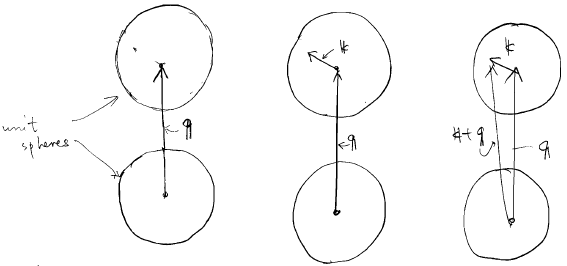
\includegraphics[width=0.6\textwidth]{2-8-20.png}
\end{center}
\begin{itemize}
\item We consider the vector $\mathbf{k}$ from the center of this unit sphere.

\item Then a vector, which connects this point and the other center is nothing but $\mathbf{k}+\mathbf{q}$.

\item These two factors require that the allowed integral region for $\mathbf{k}$ is within this unit sphere, while $\mathbf{k}$ should be outside the other unit sphere.

\item In this picture, these two conditions are always compatible, so that $\mathbf{k}$ can be freely integrated within this sphere.
\end{itemize}

\begin{center} \label{Fig2.8.21}
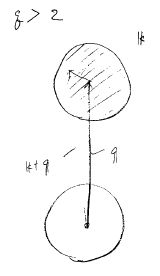
\includegraphics[width=0.17\textwidth]{2-8-21.png}
\end{center}
\begin{itemize}
\item This situation holds true, whenever the amplitude of $\mathbf{q}$ is greater than 2.
\end{itemize}

\begin{center} \label{Fig2.8.22}
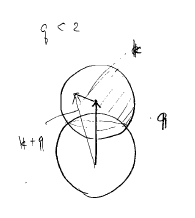
\includegraphics[width=0.2\textwidth]{2-8-22.png}
\end{center}
\begin{itemize}
\item Otherwise, these two unit spheres have a finite overlap, where the integral region for $\mathbf{k}$ is restricted within this shadow region.
\end{itemize}

Let us first consider $q>2$ case.

In such a case, this part is bounded by this form:\footnote{equality holds true when $|\mathbf{k}|=1,\mathbf{k}\cdot \mathbf{q} < 0, \mathbf{k} \parallel \mathbf{q}$ or $|\mathbf{k}|=1,\mathbf{k}\cdot \mathbf{q} > 0, \mathbf{k} \parallel \mathbf{q}$}
\[ -q + \frac{q^2}{2} \leq \mathbf{k}\cdot\mathbf{q}+\frac{q^2}{2} \leq q+ \frac{q^2}{2} \]

As such, the right hand side remains finite, only when $\nu$ is within this regions.
\[ \underline{-q + \frac{q^2}{2} < \nu < q + \frac{q^2}{2}} \]

Otherwise, $Im\Pi^0(\mathbf{q},\nu)$ always reduces to zero.

If this(underlined) is the case, the integrand remains finite only when $k$ is within the plane which satisfies $\frac{q^2}{2}+\mathbf{q}\cdot \mathbf{k} = \nu$,
\begin{center} \label{Fig2.8.23}
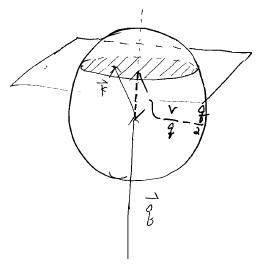
\includegraphics[width=0.35\textwidth]{2-8-23.png}
\end{center}

where the distance between this plane and the center of this unit sphere is given by
\[ k_d = |\frac{\nu}{q} - \frac{q}{2}| \]

With this in mind, we have
\begin{equation} \label{Eqs2.8.21} \begin{split}
Im\Pi^0(\mathbf{q},\nu) =& -\frac{m k_F}{4\pi^2 \hbar^2} 2\pi \int_{|\frac{\nu}{q}-\frac{q}{2}|}^1 k^2 \cdot \mathrm{d}k \int_{-1}^{+1} \mathrm{d}t \delta(\nu-qkt -\frac{q^2}{2})\\
=& -\frac{m k_F}{4\pi^2 \hbar^2} 2\pi \int_{|\frac{\nu}{q}-\frac{q}{2}|}^1 k^2 \cdot \mathrm{d}k \int_{-1}^{+1} \mathrm{d}t \frac{1}{qk}\delta(t - \frac{\nu}{qk} + \frac{q}{2k})\\
=&-\frac{m k_F}{4\pi^2 \hbar^2} \frac{2\pi}{q} \left[ \frac{k^2}{2} \right]_{k=|\frac{\nu}{q}-\frac{q}{2}|}^{k=1}\\
=&-\frac{m k_F}{\hbar^2} \cdot \frac{1}{4\pi} \left[ 1-\left( \frac{\nu}{q}-\frac{q}{2} \right)^2 \right]
\end{split}\end{equation}

Let us next consider $q<2$ case.
\begin{center}\label{Fig2.8.24}
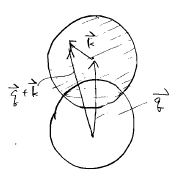
\includegraphics[width=0.17\textwidth]{2-8-24.png}
\end{center}

In this case, the integration over $k$ is restricted within this shaded region.

In such a case, this part($\frac{q^2}{2} + \mathbf{q} \cdot \mathbf{k}$) is bounded by this form
\[ 0 \leq \frac{q^2}{2} + \mathbf{q} \cdot \mathbf{k} \leq \frac{q^2}{2} + q \]
\begin{center}\label{Fig2.8.25}
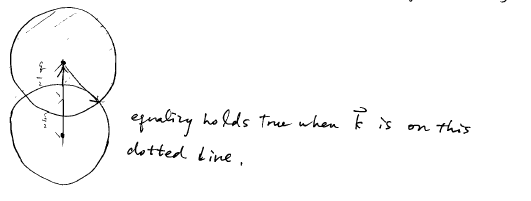
\includegraphics[width=0.6\textwidth]{2-8-25.png}
\end{center}

Therefore, the integral remains finite only when $\nu$ is bounded by this region
\[ 0 \leq \nu \leq \frac{q^2}{2} + q \]

To perform this integral explicitly, it is technically useful to divide this region into these two regions.
\begin{enumerate}[(i)]
\item $q-\frac{q^2}{2} \leq \nu(=\frac{q^2}{2}+\mathbf{q}\cdot\mathbf{k}) \leq \frac{q^2}{2} + q$
\item $0\leq \nu(=\frac{q^2}{2}+\mathbf{q}\cdot\mathbf{k}) \leq q - \frac{q^2}{2}$
\end{enumerate}

When $\mathbf{k}$ is along the plane which touches with this lower unit sphere, this term becomes equal to this quantity.
\begin{center}\label{Fig2.8.26}
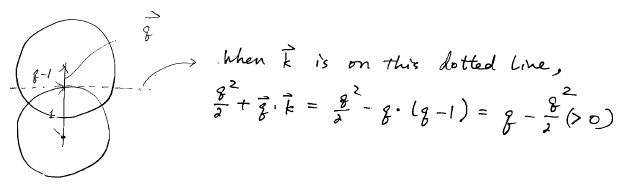
\includegraphics[width=0.6\textwidth]{2-8-26.png}
\end{center}

In the former case, the integral can be performed exactly in the same way as we did for $q>2$ case.
\begin{equation} \label{Eqs2.8.22} \begin{split}
Im\Pi^0(q,\nu) =& -\frac{m k_F}{4\pi^2 \hbar^2} 2\pi \int_{|\frac{\nu}{q} - \frac{q}{2}|}^{1} k^2  \cdot \mathrm{d} k \int_{-1}^{1} \mathrm{d} t \delta(\nu - qkt - \frac{q^2}{2})\\
=& - \frac{m k_F}{\hbar^2}\frac{1}{4\pi} \left[ 1-\left( \frac{\nu}{q}-\frac{q}{2} \right)^2 \right]
\end{split}\end{equation}

In the latter case, the integration becomes a little involved, bacause the plane also enters inside the lower unit sphere, which is the forbidden region.
\[ Im\Pi^0(\mathbf{q},\nu) = -\frac{m k_F}{(2\pi \hbar)^2} \int \mathrm{d}^3 k \cdot \theta(1-|k|) \theta(|\mathbf{q}+\mathbf{k}|-1) \delta(\nu-\mathbf{q}\cdot\mathbf{k}-\frac{q^2}{2})
\]

\begin{center}\label{Fig2.8.27}
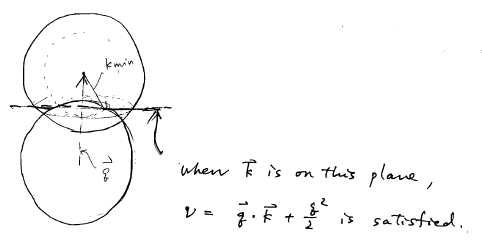
\includegraphics[width=0.6\textwidth]{2-8-27.png}
\end{center}

When $\mathbf{k}$ is within this shaded annulus, the integrand remains finite.

Thus we define $k_{min}$ as a distance between the center of the upper sphere and the inner boundary of the annulus.

In terms of $k_{min}$ thus defined, the integral is given by
\[ Im\Pi^0(\mathbf{q},\nu) = - \frac{m k_F}{\hbar^2}\frac{1}{2\pi} \int_{k_{min}}^1 k^2  \cdot \mathrm{d} k \int_{-1}^1 \mathrm{d} t \cdot \delta(\nu-qkt-\frac{q^2}{2})\]

By a simple geometry, $k_{min}$ is given by $\nu$ as follows:
\[ k_{min} = (1-2\nu)^{\frac{1}{2}} \]
\begin{center}\label{Fig2.8.28}
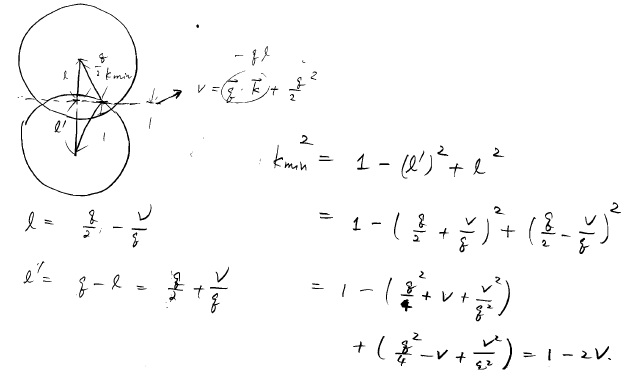
\includegraphics[width=0.6\textwidth]{2-8-28.png}
\end{center}

Thus
\begin{equation} \label{Eqs2.8.23} \begin{split}
 Im\Pi^0(\mathbf{q},\nu) =& - \frac{m k_F}{\hbar^2}\frac{1}{2\pi q} \int_{(1-2\nu)^{\frac{1}{2}}}^1 k  \cdot \mathrm{d} k \int_{-1}^1 \mathrm{d} t \cdot \delta(\frac{\nu}{qk}-\frac{q}{2 k}-t)\\
=& - \frac{m k_F}{\hbar^2}\frac{1}{2\pi q} \left[ \frac{k^2}{2} \right]_{k=(1-2\nu)^{\frac{1}{2}}}^{k=1}\\
=& - \frac{m k_F}{\hbar^2}\frac{1}{4\pi q} \left[ 1 - (1-2\nu) \right]\\
=& - \frac{m k_F}{\hbar^2}\frac{1}{4\pi q} 2\nu
\end{split}\end{equation}

To summarize, so far, the imaginary part can be given as follows
\begin{equation} \label{Eqs2.8.24}
\text{Im} \Pi^0(q,\nu) = \left\{ \begin{split}
&-\frac{m k_F}{\hbar^2} \frac{1}{4\pi q} \left[ 1-\left( \frac{\nu}{q} - \frac{q}{2} \right)^2 \right] \qquad \left( \begin{split}
&(i) q > 2 \quad\&\quad \frac{q^2}{2} - q\leq \nu \leq \frac{q^2}{2} + q\\
&or\\
&(ii) q < 2 \quad\&\quad -\frac{q^2}{2} + q \leq \nu \leq \frac{q^2}{2} + q
\end{split}  \right)\\
&-\frac{m k_F}{\hbar^2} \frac{1}{4\pi q} 2\nu \qquad 
\left( (iii) q < 2 \quad\&\quad 0 \leq \nu \leq -\frac{q^2}{2}+q \right)\\
&0\qquad  (otherwise)
\end{split} \right.
\end{equation}

When viewed as a function of $\nu$, the Imaginary part can be drawn like this:

\begin{itemize}
\item For $(0 < ) q < 2$ case:
\begin{center}\label{Fig2.8.29}
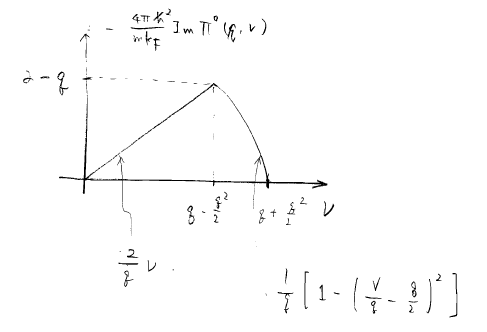
\includegraphics[width=0.6\textwidth]{2-8-29.png}
\end{center}
\item For $2 < q$ case:
\begin{center}\label{Fig2.8.30}
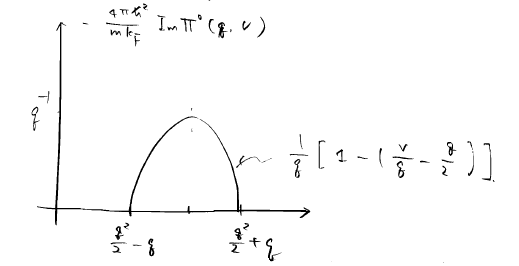
\includegraphics[width=0.6\textwidth]{2-8-30.png}
\end{center}
\end{itemize}

For many applications, it is useful to enumerate limiting forms of $\Pi^0(\mathbf{q},\nu)$:
\begin{itemize}
\item One is called as a static limit, in which we take $\nu$ to be zero, while $q$ is fixed:

\begin{center}Fixed $q$, while $\nu \rightarrow 0$.\end{center}

In these two graphs, this limit corresponds to approaching the origin in \underline{this way} or approaching the origin in \underline{this way}.

Therefore, $Im\Pi^0(\mathbf{q},\nu)$ reduces to zero in this limit.
\begin{equation} \label{Eqs2.8.25.a} \tag{2.8.25.a}
Im\Pi^0(\mathbf{q},\nu) = 0
\end{equation}
\setcounter{equation}{25}

The real part of $\Pi^0(\mathbf{q},\nu)$ can be also easily calculated from eq.(F)
\begin{equation*} \label{Eqs2.8.25.b} \tag{2.8.25.b}
Re\Pi^0(\mathbf{q},\nu) = \frac{m k_F}{\hbar^2}\cdot \frac{1}{2\pi^2} \times \left\{ -1 + \frac{1}{q}(1-\frac{q^2}{4})log\left( \frac{1-\frac{q}{2}}{1+\frac{q}{2}} \right) \right\}
\end{equation*}

\item Another physically important limit is the dynamic limit, in which we take $q$ to be zero, with fixed $\nu$:

\begin{center}Fixed $\nu$, while $q\rightarrow 0$\end{center}

When $q$ goes to zero, these upper bounds and lower bounds go to zero.

Since we fix $\nu$ to be finite, this limit ends up in outside of these regions, where the imaginary part reduces to zero.
\begin{equation*} \label{Eqs2.8.26.a} \tag{2.8.26.a}
Im\Pi^0(\mathbf{q},\nu) = 0
\end{equation*}
\setcounter{equation}{26}

To calculate the real part in the dynamical limit, we need to Taylor-expand this logarithmic part in small $q$:
\[log\left( \frac{\nu+q\mp\frac{q^2}{2}}{\nu-q\mp\frac{q^2}{2}}\right) = \frac{2 q}{\nu}\pm\frac{q^3}{\nu^2}+\frac{2}{3}\frac{q^3}{\nu^3}+\frac{q^5}{2\nu^3}\pm\frac{q^5}{\nu^4}+\frac{2}{5}\frac{q^5}{\nu^5}+o(q^7) \]

In terms of these expansions, eq.(\ref{Eqs2.8.20}) can be calculated as
\[ \begin{split}
Re\Pi^0(\mathbf{q},\nu) =& \frac{2 m k_F}{\hbar^2}\cdot \frac{1}{4\pi^2} \times\\
&\left\{ -1 + \frac{1}{2q} \left( 1- (\frac{\nu}{q})^2+\nu-\frac{q^2}{4} \right) \times  \left( \frac{2 q}{\nu}+\frac{q^3}{\nu^2}+\frac{2}{3}\frac{q^3}{\nu^3}+\frac{q^5}{2\nu^3}+\frac{q^5}{\nu^4}+\frac{2}{5}\frac{q^5}{\nu^5} \right)\right.\\
&\left.-\frac{1}{2q}\left( 1- (\frac{\nu}{q})^2-\nu-\frac{q^2}{4} \right) \times \left( \frac{2 q}{\nu}-\frac{q^3}{\nu^2}+\frac{2}{3}\frac{q^3}{\nu^3}+\frac{q^5}{2\nu^3}-\frac{q^5}{\nu^4}+\frac{2}{5}\frac{q^5}{\nu^5} \right)\right\}\\
=&\frac{2 m k_F}{\hbar^2}\cdot \frac{1}{4\pi^2} \times\\
&\left\{ -1 + \frac{1}{2q}\left( 1-(\frac{\nu}{q})^2-\frac{q^2}{4} \right) \times \left( \frac{2 q^3}{\nu^2}+\frac{2 q^5}{\nu^4} \right) + \frac{\nu}{2q}\left( \frac{4 q}{\nu} + \frac{4 q^3}{3 \nu^3} + o(q^5) \right) \right\}\\
=&\frac{2 m k_F}{\hbar^2}\cdot \frac{1}{4\pi^2} \times \left\{ -1 -1 + 2 + \frac{2}{3}\frac{q^2}{\nu^2}+o(q^4) \right\}
\end{split}\]
\begin{equation*}\label{Eqs2.8.26.b}\tag{2.8.26.b}
Re\Pi^0(\mathbf{q},\nu) = \frac{2 m k_F}{\hbar^2}\cdot \frac{1}{4\pi^2} \cdot \frac{2}{3}\frac{q^2}{\nu^2} + o(q^4)
\end{equation*}

\item The third limit is an intermediate limit between the static limit \& the dynamic limit.

More specifically, we take $q$ \& $\nu$ to be zero simultaneously, while the ratio between $q$ and $\nu$ to be fixed:

\begin{center}Fixed $\frac{\nu}{q} \equiv x$, while $q\rightarrow 0$ \end{center}

This limit corresponds to this case, so that the imaginary part is given by
\[ Im\Pi^0(q,v=q x) = \left\{ \begin{split}&-\frac{m k_F}{\hbar^2} \cdot \frac{1}{4\pi q} 2\nu \quad (0\leq \nu \leq q)\\
&0 \quad (q \leq \nu) \end{split} \right. \]

\begin{equation*} \label{Eqs2.8.27.a} \tag{2.8.27.a}
\text{Im} \Pi^0(q,\nu=q x) = -\frac{m k_F}{\hbar^2}\frac{x}{2\pi} \theta(1-x)
\end{equation*}
\setcounter{equation}{27}

To calculate the real part, we taylor-expand these logarithmic parts in small $q$, while $\frac{\nu}{q}$ being regarded as a constant:
\[log\left| \frac{1+\frac{\nu}{q}-\frac{q}{2}}{1-\frac{\nu}{q}+\frac{q}{2}} \right| = \log \left| \frac{1+\frac{\nu}{q}}{1-\frac{\nu}{q}} \right| - \frac{\frac{q}{2}\cdot 2}{1-(\frac{\nu}{q})^2} + o(q^2)\]

\[log\left| \frac{1+\frac{\nu}{q}+\frac{q}{2}}{1-\frac{\nu}{q}-\frac{q}{2}} \right| = \log \left| \frac{1+\frac{\nu}{q}}{1-\frac{\nu}{q}} \right| + \frac{\frac{q}{2}\cdot 2}{1-(\frac{\nu}{q})^2} + o(q^2)\]

Uing these expansions, we obtain the leading order expression for the real part as follows:
\[ \begin{split}Re\Pi^0(\mathbf{q},\nu=q x) =& \frac{2m k_F}{\hbar^2} \frac{1}{4\pi^2} \times\\
&\left\{ -1 + \frac{1}{2q}\left( 1-(\frac{\nu}{q})^2+\nu-\frac{q^2}{4} \right) \times \left( \log \left| \frac{1+\frac{\nu}{q}}{1-\frac{\nu}{q}} \right| - \frac{q}{1-(\frac{\nu}{q})^2} + o(q^2) \right) \right.\\
&\left.-\frac{1}{2q}\left( 1-(\frac{\nu}{q})^2-\nu-\frac{q^2}{4} \right) \times \left( \log \left| \frac{1+\frac{\nu}{q}}{1-\frac{\nu}{q}} \right| + \frac{q}{1-(\frac{\nu}{q})^2} + o(q^2) \right)\right\}\\
=&\frac{m k_F}{\hbar^2} \frac{1}{2\pi^2}\left\{ -1 + \frac{\nu}{2q}log\left| \frac{1+\frac{\nu}{q}}{1-\frac{\nu}{q}} \right| \times 2 - 1 + o(q) \right\}
\end{split}\]
\begin{equation*} \label{Eqs2.8.27.b} \tag{2.8.27.b}
Re\Pi^0(\mathbf{q},\nu=q x)=\frac{m k_F}{\hbar^2} \frac{1}{2\pi^2} \left\{ -2 + x\cdot \log\left| \frac{1+x}{1-x} \right|+ o(q) \right\}
\end{equation*}
\end{itemize}

\begin{center}--------------------\end{center}

Using these expressions for the zero-th order proper polarization part, let us next calculate the dielectric constant given within the ring-diagram approximation.

Namely, using eq.(\ref{Eqs2.8.10}), we have
\begin{equation} \label{Eqs2.8.28} \begin{split}
K_r(k_F \mathbf{q}, \omega= \frac{\hbar k_F^2}{m}\nu) =& 1- V(k_F \mathbf{q}) \Pi^0(\mathbf{q},\nu)\\
=& 1- \frac{4\pi e^2}{k_F^2}\frac{1}{q^2} \left( Re\Pi^0(\mathbf{q},\nu)+i Im\Pi^0(\mathbf{q},\nu) \right)
\end{split}\end{equation}

where the real part and imaginary part are given in eq.(\ref{Eqs2.8.20}) \& eq.(\ref{Eqs2.8.24}) respectively.

\begin{itemize}
\item In the static limit, the dielectric constant thus obtained takes the following asymptotic form:
\item \begin{center}static limit ($\nu \rightarrow 0$, while fixing $q$)\end{center}

\begin{equation} \label{Eqs2.8.29}
K_r(q,0) = 1-\underline{\frac{4\pi e^2}{k_F^2}} \frac{1}{q^2} \cdot \underline{\frac{m k_F}{\hbar^2} \frac{1}{2\pi^2}} \times \left\{ -1 + \frac{1}{q}\left( 1-\frac{q^2}{4} \right)log\left| \frac{1-\frac{q}{2}}{1+\frac{q}{2}} \right| \right\}
\end{equation}

The underlined coefficient part is proportional to a ratio between Fermi wavelength and Bohr radius.
\begin{equation} \label{Eqs2.8.30} \begin{split}
\frac{4\pi e^2}{k_F^2}\cdot\frac{m k_F}{\hbar^2} \frac{1}{2\pi^2} =& \frac{2}{\pi}\cdot\frac{1}{k_F}\cdot\frac{m e^2}{\hbar^2} = \frac{2}{\pi} \frac{1}{k_F}\frac{1}{a_B}\\
=& \frac{1}{\pi^2}\frac{\lambda_F}{a_B}
\end{split}\end{equation}

Fermi wavelength is proportional to the interparticle spacing in degenerate electron gas:
\begin{equation} \label{Eqs2.8.31}
\lambda_F = \frac{2\pi}{k_F} = 2\pi \left( \frac{4}{9\pi} \right)^{\frac{1}{3}} r_0 \equiv 2\pi \alpha r_0
\end{equation}

Thus, this coefficient is a dimensionless quantity which measures the density of a degenerate electron gas.
\begin{equation} \label{Eqs2.8.32}
=\frac{2}{\pi} \alpha (\frac{r_0}{a_B}) \equiv \frac{2}{\pi} \alpha r_S
\end{equation}

Especially, the ratio between the interparticle spacing and Bohr radius is often called as $r_S$, which plays role of the most important coupling constant in a degenerate electron gas.

By its definition, $r_S$ goes to zero in the high-density limit, while $r_S$ goes infinity in the low-density limit.
\[ r_S \rightarrow 0 \qquad\text{(high-density limit)} \]

In terms of $r_S$, the dielectric constant in the static limit is given by
\begin{equation} \label{Eqs2.8.33}
K_r(q,0) = 1+ \frac{2\alpha r_S}{\pi q^2}\left[ 1-\frac{1}{q}(1-\frac{q^2}{4})ln\left| \frac{1-\frac{q}{2}}{1+\frac{q}{2}} \right| \right]
\end{equation}

\item In the dynamic limit, the dielectric constant is given as follows within the ring-diagram approximation:
\item \begin{center}dynamic limit($q \rightarrow 0$, while fixing $\nu$)\end{center}
\begin{equation} \label{Eqs2.8.34} \begin{split}
K_r(0,\nu) =& 1- \frac{4\pi e^2}{k_F^2} \frac{1}{q^2}\frac{2 m k_F}{\hbar^2} \cdot \frac{1}{4\pi^2} \frac{2}{3}\frac{q^2}{\nu^2}\\
=& 1- \frac{4\alpha r_S}{3\pi \nu^2}
\end{split}\end{equation}

\item In the intermediate limit, the dielectric constant takes the following  asymptotic form:
\begin{equation} \label{Eqs2.8.35} \begin{split}
K_r(q,qx) =& 1-\frac{4\pi e^2}{k_F^2}\frac{1}{q^2} \times \left\{ - \frac{m k_F}{\hbar^2}\cdot\frac{1}{2\pi^2}\left( 2-x \ln\left| \frac{1+x}{1-x} \right| \right) - \frac{m k_F}{\hbar^2}\cdot \frac{x}{2\pi} i \theta(1-x) \right\}\\
=& 1+ \frac{4 \alpha r_S}{\pi q^2}\left( 1-\frac{x}{2} \ln\left| \frac{1+x}{1-x} \right|  \right) + \frac{2 i \alpha r_S}{q} x \theta(1-x)
\end{split}\end{equation}

\end{itemize}

These three expressions for the dielectric constant turns out to be very useful to understand physical properties of high-density degenerate electron gas.

In the latter sections, we will use these expressions, in order to understand many important properties of the degenerate electron gas.
\begin{center}----------------------------\end{center}

In the remain part of this section, we will go back to the evaluation of correlation energy within the ring-diagram approximation.

For its comparison, we will also evaluate the second-order term.
\begin{equation*} \tag{2.8.9}
E_r = \frac{1}{2}i V\hbar \int \frac{\mathrm{d}^4 q}{(2\pi)^4} \int_0^1 \mathrm{d} \lambda \cdot \lambda^{-1} \frac{[\lambda V_0(q) \Pi^0(q)]^2}{1-\lambda V_0(q) \Pi^0(q)}
\end{equation*}

\begin{equation*} \label{Eqs2.8.9.a} \tag{2.8.9.a}
E_2^r = \frac{1}{2}i V \hbar\int \frac{\mathrm{d}^4 q}{(2\pi)^4} \int_0^1 \mathrm{d} \lambda \cdot \lambda^{-1}  \left[ \lambda V_0(q)\Pi^0(q) \right]^2
\end{equation*}

Equivalently
\begin{center} \label{Fig2.8.31}
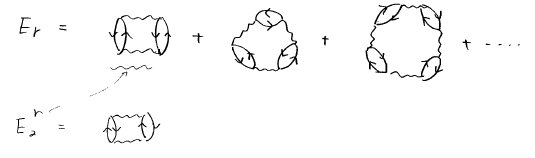
\includegraphics[width=0.6\textwidth]{2-8-31.png}
\end{center}

Let us begin with the 2nd-order term first:
\[E_2^r = \frac{1}{4}i V \hbar\int \frac{\mathrm{d}^3 \mathbf{q}}{(2\pi)^3} \int_{-\infty}^{+\infty} \frac{\mathrm{d} \omega}{2\pi} V_0^2(\mathbf{q})  \left[ \Pi^0(\mathbf{q},\omega) \right]^2\]

As before, we introduce dimensionless frequency and momentum
\begin{equation*} \tag{2.8.18}
\nu = \frac{m}{\hbar k_F^2} \omega, \quad \mathbf{q}_{new} = \frac{\mathbf{q}_{old}}{k_F}
\end{equation*}

In terms of these new variables, $E_2^r$ is given as follows
\[\begin{split}E_2^r =& \frac{1}{4}i V \hbar \frac{k_F^3}{16\pi^4} \frac{\hbar k_F^2}{m}
\int \mathrm{d}^3 \mathbf{q} \int \mathrm{d} \nu \cdot [V_0 \Pi^0]^2\\
\xlongequal{k_F^3 = \frac{3\pi^2 N}{V}}& \frac{1}{4}i\frac{\hbar^2 k_F^2}{m e^2}\cdot \frac{3 e^2 N}{16 \pi^2}
\int \mathrm{d}^3 \mathbf{q} \int \mathrm{d} \nu \cdot [V_0 \Pi^0]^2\\
\xlongequal{\frac{\hbar^2}{m e^2}=a_0}& \frac{N e^2}{2 a_0} \left( \frac{3i}{32\pi^2}(k_F a_0)^2 \int \mathrm{d}^3 \mathbf{q} \int \mathrm{d} \nu \left[ V_0 \Pi^0 \right]^2 \right)
\end{split}\]

\begin{equation*} \label{Eqs2.8.9.b} \tag{2.8.9.b}
E_2^r = \frac{N e^2}{2 a_0} \left( \frac{3i}{16\pi^2 (\alpha r_S)^2} \int \mathrm{d}^3 \mathbf{q} \int_0^{+\infty} \mathrm{d} \nu \left[ V_0 \Pi^0 \right]^2 \right)
\end{equation*}

expressions for the polarization part obtained in the dynamic limit and the intermediate limit.

One can also confirm that the expression in the intermediate limit(eq.(\ref{Eqs2.8.27.a}) \& eq.(\ref{Eqs2.8.27.b})), includes that of the dynamic limit(eq.(\ref{Eqs2.8.26.a}) \& eq.(\ref{Eqs2.8.26.b})) as a limiting situation.

Therefore, we may use the expression obtained in the intermediate limit,
\[\left\{ \begin{split}
\text{Im} \Pi^0(|\mathbf{q}|, \nu = |\mathbf{q}| x) =& - \frac{m k_F}{\hbar^2} \frac{x}{2\pi} \theta(1-x)\\
\text{Re} \Pi^0(|\mathbf{q}|, \nu = |\mathbf{q}| x) =& \frac{m k_F}{\hbar^2}\frac{1}{2\pi^2}\left\{ -2 + x \ln\left| \frac{1+x}{1-x} \right| \right\}
\end{split} \right.\]

Now that the energy must be always real-valued, we only focus on the real part of the right hand side.

As mentioned before, $E_2^r$ diverges logarithmically due to the singular behaviour of the Coulomb potential: $V_0(q) = \frac{4\pi e^2}{q^2}$ around $q=0$.

To see this situation, let us separate the momentum integral into two parts:
\[ \epsilon_2^r = \frac{3i}{16\pi^2 \alpha^2 r_S^2} \left( \int_{|\mathbf{q}|<q_c} \mathrm{d}^3 \mathbf{q} + \int_{|\mathbf{q}|>q_c} \mathrm{d}^3 \mathbf{q} \right) \int_0^{+\infty} \mathrm{d} \nu \cdot V_0^2(\mathbf{q}) {\Pi^0}^2(\mathbf{q},\nu) \]

and let us focus only on the first integral.
\begin{equation*} \label{Eqs2.8.9.c} \tag{2.8.9.c}
\epsilon_2^{r,1} = \frac{3i}{16\pi^2 \alpha^2 r_S^2} \int_{|\mathbf{q}|<q_c} \mathrm{d}^3 \mathbf{q} \int_0^{+\infty} \mathrm{d} \nu \cdot V_0^2(\mathbf{q}) {\Pi^0}^2(\mathbf{q},\nu)
\end{equation*}

When $q_c$ is chosen to be much smaller than $1$, we may approximately employ the
\footnote{$\left(\frac{m k_F}{\hbar^2}\right)^2\left( \frac{4\pi e^2}{k_F^2} \right)^2 = \left( \frac{4\pi}{k_F a_0} \right)^2 = (4\pi)^2(\alpha r_S)^2$}
\footnote{$f(x)=\frac{2}{\pi} \left\{ 1 - \frac{x}{2} \ln\left| \frac{1+x}{1-x} \right| \right\}$}

\[\begin{split}
\epsilon_2^{r,1} =& -\frac{3}{8\pi^2 \alpha^2 r_S^2} \int_{|\mathbf{q}|<q_c} \mathrm{d}^3 \mathbf{q} \int_0^{+\infty} \mathrm{d} \nu \cdot V_0^2(\mathbf{q}) Re\Pi^0(\mathbf{q},\nu) Im\Pi^0(\mathbf{q},\nu)\\
=&-\frac{3}{2\pi \alpha^2 r_S^2} \int_0^{q_c} q^2 \cdot \mathrm{d} q \int_0^{+\infty} \mathrm{d} (q x) \cdot V_0^2(\mathbf{q}) \times Re\Pi^0(\mathbf{q},q x) Im\Pi^0(\mathbf{q},q x)\\
=& -\frac{6}{\pi} \int_0^{q_c} q^3 \cdot \mathrm{d} q \int_0^{+\infty} \mathrm{d} x \cdot \frac{1}{q^4} x \frac{2}{\pi} \left\{ 1 - \frac{x}{2} \ln\left| \frac{1+x}{1-x} \right| \right\} \theta(1-x)
\end{split}\]

\begin{equation*} \label{Eqs2.8.9.d} \tag{2.8.9.d}
\epsilon_2^{r,1}= -\frac{6}{\pi} \int_0^{q_c} \frac{1}{q} \cdot \mathrm{d} q \int_0^{1} \mathrm{d} x \cdot  x f(x)
\end{equation*}

From this final expression, we can see that this momentum integral exhibits logarithmic divergence in the infrared regime.

Moreover, when it comes to the 3rd-order term\includegraphics[width=0.15\textwidth]{2-8-32.png}, the integrand contains $V_0^3(q) (\Pi^0(q))^3$, so that this momentum integral in the infrared regime will be replaced by the following form.
\begin{equation*} \label{Eqs2.8.9.e} \tag{2.8.9.e}
\int_0^{q_c}q^3 \cdot \frac{1}{q^6} \cdot \mathrm{d}q \int_0^1 \mathrm{d} x \left( a x f^2(x) + bx^3 \right)
\end{equation*}

which exhibits more singular divergence at $q=0$.

An idea of ``ring-diagram approximation" is to sum up all these singular terms up to all order in the perturbation theory:
\begin{center} \label{Fig2.8.33}
\includegraphics[width=0.6\textwidth]{2-8-33.png}
\end{center}
\begin{equation*} \tag{2.8.9}
E_r = \frac{1}{2}i V\hbar \int \frac{\mathrm{d}^4 q}{(2\pi)^4} \int_0^1 \mathrm{d} \lambda \cdot \lambda \frac{[ V_0(q) \Pi^0(q)]^2}{1-\lambda V_0(q) \Pi^0(q)}
\end{equation*}

Remarkably, when summed over up to all order, these singularities cancel each other, which results in a finite contribution.

To see this situation, let us next calculate $E_r$:
\[\begin{split}
E_r =& \frac{1}{2}i V\hbar \int \frac{\mathrm{d}^4 q}{(2\pi)^4} \int_0^1 \mathrm{d} \lambda \cdot \lambda \frac{V_0^2 {\Pi^0}^2}{1-\lambda V_0\Pi^0}\\
=& \frac{1}{2}i V\hbar \int \frac{\mathrm{d}^4 q}{(2\pi)^4} \int_0^1 \mathrm{d} \lambda V_0 \Pi^0\left( -1 + \frac{1}{1-\lambda V_0 \Pi^0} \right)\\
=& - \frac{1}{2}i V\hbar \int \frac{\mathrm{d}^4 q}{(2\pi)^4}\left[\left( \log[1-\lambda V_0 \Pi^0] \right)_{\lambda=0}^{\lambda=1} + V_0 \Pi^0 \right]\end{split}\]
\begin{equation*} \label{Eqs2.8.9'} \tag{2.8.9'} \begin{split}
E_r=& - \frac{1}{2}i V\hbar \int \frac{\mathrm{d}^3 \mathbf{q}}{(2\pi)^3} \int \frac{\mathrm{d} \omega}{2\pi} \left\{ \log[1-V_0 \Pi^0] + V_0 \Pi^0 \right\}\\
=& - \frac{1}{2}i V\hbar \int \frac{\mathrm{d}^3 \mathbf{q}}{(2\pi)^3} \int \frac{\mathrm{d} \omega}{2\pi} \left\{ \log[K_r(\mathbf{q},\omega)] + 1-K_r(\mathbf{q},\omega) \right\}
\end{split}\end{equation*}

Using the dimensionless frequency and momentum, this can be given by the dimensionless integral.
\begin{equation} \label{Eqs2.8.36}
E_r = \frac{N e^2}{2 a_0} \epsilon_r
\end{equation}

\[\begin{split} \epsilon_r = -\frac{3i}{16\pi^2 \alpha^2 r_S^2} \int \mathrm{d}^3 \mathbf{q}^{'}\int_{-\infty}^{+\infty} \mathrm{d}\nu \left\{ \log K_r(q^{'},\nu) + 1-K_r(q^{'},\nu) \right\}\\\text{(with $\mathbf{q}^{'} = \frac{\mathbf{q}}{k_F}$, $\nu = \frac{m}{\hbar k_F^2} \omega$)}\end{split} \]

Since $K_r$ depends on the norm of $\mathbf{q}^{'}$ and it is an even function of $\nu$, we have
\[ \epsilon_r = -\frac{3i}{2\pi \alpha^2 r_S^2} \int_0^{+\infty} {q^{'}}^2 \cdot \mathrm{d}q^{'} \int_{0}^{+\infty} \mathrm{d}\nu \left\{ \log K_r(q^{'},\nu) + 1-K_r(q^{'},\nu) \right\}\]

The energy must be real-valued, so that we focus only on the imginary part of this parenthesis.
\begin{equation} \label{Eqs2.8.37}
\epsilon_r = \frac{3}{2\pi \alpha^2 r_S^2} \int_0^{+\infty} q^2 \cdot \mathrm{d}q \int_0^{+\infty} \mathrm{d}\nu \left\{ tan^{-1}\left( \frac{\text{Im} K_r(q,\nu)}{\text{Re} K_r(q,\nu)} \right) - \text{Im} K_r(q,\nu) \right\}
\end{equation}

with
\begin{equation} \label{Eqs2.8.38}
log(\text{Re} K + i \text{Im} K) = \log \sqrt{\text{Re} K^2 + \text{Im} K^2} + i tan^{-1} \left( \frac{\text{Im} K}{\text{Re} K} \right)
\end{equation}

In order to see how the singular behaviour of the integrand at $q=0$ is removed by the summation of the ring-diagrams, we separate this momentum integral into two parts:
\begin{eqnarray}
\epsilon_r =& \epsilon_{r,1} + \epsilon_{r,2} \nonumber\\
\epsilon_{r,1} =& \frac{3}{2\pi \alpha^2 r_S^2} \int_0^{q_c} q^2 \cdot \mathrm{d} q \int_0^{+\infty} \mathrm{d} \nu \left\{ tan^{-1}\left( \frac{\text{Im} K}{\text{Re} K} \right) - \text{Im} K  \right\} \label{Eqs2.8.39}\\
\epsilon_{r,2} =& \frac{3}{2\pi \alpha^2 r_S^2} \int_{q_c}^{+\infty} q^2 \cdot \mathrm{d} q \int_0^{+\infty} \mathrm{d} \nu \left\{ tan^{-1}\left( \frac{\text{Im} K}{\text{Re} K} \right) - \text{Im} K  \right\} \label{Eqs2.8.40}
\end{eqnarray}

$\epsilon_{r,2}$ is free from infrared divergence, so that it results in a finite contribution.

Toevaluate $\epsilon_{r,1}$, we again choose $q_c$ to be sufficiently smaller than 1, so that the integrand can be evaluated in terms of eqs.
\begin{equation} \label{Eqs2.8.41} \begin{split}
\epsilon_{r,1} =& \frac{3}{2\pi \alpha^2 r_S^2}\int_0^{q_c} q^3\cdot \mathrm{d} q \int_0^{+\infty} \mathrm{d} x \left\{ tan^{-1}\left[ \frac{2\alpha r_S x \theta(1-x)}{q^2+2\alpha r_S f(x)} \right] - \frac{2\alpha r_S x \theta(1-x)}{q^2} \right\}\\
=& \frac{3}{2\pi \alpha^2 r_S^2}\int_0^{q_c} q^3 \cdot \mathrm{d} q \int_0^{1} \mathrm{d} x \left\{ tan^{-1}\left[ \frac{2\alpha r_S x}{q^2+2\alpha r_S f(x)} \right] - \frac{2\alpha r_S x}{q^2} \right\}\\
&+\frac{3}{2\alpha^2 r_S^2} \int_0^{q_c} q^3 \cdot\mathrm{d}q \int_1^{+\infty} \mathrm{d} x \theta(-q^2-2\alpha r_S f(x))
\end{split}\end{equation}

where $\theta$ denotes the step function:
\[\theta(x) = \left\{ \begin{split} 1 \quad x> 0\\
0 \quad x<0 \end{split} \right.\]

The second term is because $tan^{-1}(\frac{K_2}{K_1})$ takes $\pi$, when $K_2=0$ and $K_1$ is negative.

The singular behaviour of the integrand in small $q$ regime is expected from the former part.

In fact, when we expand the former term with respect to $\alpha r_S \propto e^2$, we have
\begin{equation*} \label{Eqs2.8.41'} \tag{2.8.41'}
\begin{split}=& \frac{3}{2\pi \alpha^2 r_S^2} \int_0^{q_c} q^3 \mathrm{d} q \int_0^1 \mathrm{d} x \left\{ \frac{2\alpha r_S x}{q^2} - \frac{4\alpha^2 r_S^2 x f(x)}{q^4} + \ldots - \frac{2\alpha r_S x}{q^2} \right\}\\
=& \frac{3}{2\pi} \int_0^{q_c} \mathrm{d} q \int_0^1 \mathrm{d} x \left\{ -\frac{4 x f(x)}{q} + \ldots \right\}
\end{split}\end{equation*}

where the first term is nothing but $\epsilon_2^{r,1}$(given in eq.(\ref{Eqs2.8.9.d})) which exhibits logarithmic divergence at $q=0$.

However, when we sum up all the ring-type diagram, we have this:
\[ \epsilon_{r,1} = \frac{3}{2\pi \alpha^2 r_S^2}\int_0^{q_c} q^3 \cdot \mathrm{d} q \int_0^1 \mathrm{d} x \underline{\left\{ tan^{-1}\left[ \frac{2\alpha r_S x}{q^2 + 2\alpha r_S f(x)} \right] -\frac{2\alpha r_S x}{q^2} \right\}} + \ldots \]

in which the $q^{-4}$ dependence of this underlined part is cut off for $q^2 < 2 \alpha r_S f(x)$.

This integral can be evaluated for small $r_S$ as follows:
\begin{equation} \label{Eqs2.8.42}
\epsilon_{r,1} = \frac{2}{\pi^2}(1-ln 2)ln r_S + const
\end{equation}

Here `constant' part means either some number which is free from $r_S$ or some function which reduces to zero in small $r_S$ limit.\footnote{W.Macke, Z.Naturforsh 5a:192(1950)}

Thus, the leading order contribution in the small $r_S$ limit is given by:
\[E_r = \frac{N e^2}{2 a_0} \left( \frac{2}{\pi^2} (1-ln 2) \ln r_S + const \right)\]

Later, many people calculated the subleading order correction to the correlation energy in the high density limit:
\begin{equation} \label{Eqs2.8.43}
\frac{E_{corr}}{N} = \frac{e^2}{2 a_0} \left( \frac{2}{\pi^2}(1 -ln 2) \ln r_S - 0.094 + o(r_S \ln r_S) \right)
\end{equation}

\chapter{Application to electron gas at the zero temperature}%chapter 3: wsz:all

\section{Screening effect in a degenerate electron gas}\label{s3-1}

In the preceding section, we have introduced the Dyson equation for the density-density correlation function, where the proper polarization part is calculated at the zero-th order perturbation theory.

These results are useful to understand many important physical properties of degenerate electron gas, such as screening effect \& plasma oscillation.

In this section, we will study these properties within the ring-diagram approximation.

As a preliminary for this, let us first introduce a theory of linear response to a weak external perturbation.

Consider an interacting many-particles system with a time-independent Hamiltonian
\[ i \hbar \frac{\partial}{\partial t} | \Psi_S(t) \rangle = H | \Psi_S (t) \rangle \]

$| \Psi_S (t) \rangle$ is a state vector in the Schr\"odinger picture, which is given by
\[| \Psi_S (t) \rangle = \mathrm{e}^{-i\frac{H}{\hbar}t}| \Psi_S (0) \rangle\]

Suppose that the system is perturbed at $t=t_0$, by introducing an additional time-dependent Hamiltonian
\begin{equation} \label{Eqs3.1.1}
i \hbar \frac{\partial}{\partial t} | \overline{\Psi}_S(t) \rangle = (H + H^{ex}(t))| \overline{\Psi}_S(t) \rangle
\end{equation}

This can be also solved symbolically:
\begin{equation} \label{Eqs3.1.2}
| \overline{\Psi}_S(t) \rangle = \mathrm{e}^{-i \frac{H}{\hbar}t}\hat{A}(t)  |\Psi_S(t) \rangle
\end{equation}

Here, $\hat{A}(t)$ reduces to a unit, when $t$ is less than $t_0$.
\begin{equation} \label{Eqs3.1.3}
\hat{A}(t) = 1 \quad (t \leq t_0)
\end{equation}

because
\[ H^{ex}(t) = 0 \quad (t \leq t_0) \]

substituting this solution into this Schr\"odinger's equation, we obtain the equation of motion for $\hat{A}(t)$:
\[ \mathrm{e}^{-i\frac{H}{\hbar}t}\hat{H}\hat{A}(t)|\Psi_S(0)\rangle + \mathrm{e}^{-i\frac{H}{\hbar}t}(i\hbar\frac{\partial \hat{A}(t)}{\partial t})|\Psi_S(0)\rangle = (H + H^{ex}(t))\mathrm{e}^{-i\frac{H}{\hbar}t}\hat{A}(t)|\Psi_S(0)\rangle \]

These two are set off by each other. So that we have
\begin{equation} \label{Eqs3.1.4} \begin{split}
i \hbar \frac{\partial}{\partial t}\hat{A}(t) =& \mathrm{e}^{i\frac{H}{\hbar}t}H^{ex}(t)\mathrm{e}^{-i\frac{H}{\hbar}t}\hat{A}(t)\\
\overset{def}{\equiv}& H_H^{ex}(t) \cdot \hat{A}(t)
\end{split}\end{equation}

where $H_H^{ex}(t)$ is the operator in the usual Heisenberg picture.

As we did many times in sec.\underline{    }, the equation of motion is solved in favor for $\hat{A}(t)$ iteratively:
\[ \hat{A}(t) = 1-\frac{i}{\hbar} \int_{t_0}^{t} \mathrm{d} t^{'} \hat{H}_{H}^{ex}(t^{'}) + \left( \frac{-i}{\hbar} \right)^2 \int_{t_0}^{t} \mathrm{d} t^{'} \int_{t_0}^{t^{'}} \mathrm{d} t^{''} \hat{H}_H^{ex}(t^{'}) \hat{H}_H^{ex}(t^{''}) + \ldots \]

This clearly observes the boundary condition. Since $H^{ex}(t) = 0$ for $t \leq t_0$, we can also rewrite this as
\begin{equation} \label{Eqs3.1.5}
\hat{A}(t) = 1-\frac{i}{\hbar} \int_{-\infty}^{t} \mathrm{d} t^{'} \hat{H}_{H}^{ex}(t^{'}) + \left( \frac{-i}{\hbar} \right)^2 \int_{-\infty}^{t} \mathrm{d} t^{'} \int_{-\infty}^{t^{'}} \mathrm{d} t^{''} \hat{H}_H^{ex}(t^{'}) \hat{H}_H^{ex}(t^{''}) + \ldots
\end{equation}

Correspondingly, we have
\begin{equation*} \label{Eqs3.1.5'} \tag{3.1.5'} \begin{split}
| \overline{\Psi}_S(t) \rangle =& \mathrm{e}^{-i \frac{H}{\hbar} t} | \Psi_S(0) \rangle - \frac{i}{\hbar}\mathrm{e}^{-i \frac{H}{\hbar}t} \int_{-\infty}^{t} \mathrm{d} t^{'} \hat{H}_{H}^{ex}(t^{'}) | \Psi_S(0) \rangle \\
&+ \left( \frac{-i}{\hbar} \right)^2 \mathrm{e}^{-i \frac{H}{\hbar}t} \int_{-\infty}^{t} \mathrm{d} t^{'} \int_{-\infty}^{t^{'}} \mathrm{d} t^{''} \hat{H}_H^{ex}(t^{'}) \hat{H}_H^{ex}(t^{''}) | \Psi_S(0) \rangle + \ldots
\end{split}\end{equation*}

With this in mind, we can calculate an expectation value of a physical observable at any given time t:
\begin{equation} \label{Eqs3.1.6}
\langle O(t) \rangle_{ex} = \frac{\langle \overline{\Psi}_S(t)|O_S|\overline{\Psi}_S(t)\rangle}{\langle \overline{\Psi}_S(t)|\overline{\Psi}_S(t)\rangle}
\end{equation}

The numerator is calculated as follows:
\begin{equation} \label{Eqs3.1.7}\begin{split}
\langle \overline{\Psi}_S(t)|O_S|\overline{\Psi}_S(t)\rangle = & \langle \Psi_S(0) | \left[ 1 + \frac{i}{\hbar}\int_{-\infty}^{t} \mathrm{d} t^{'} H_H^{ex}(t^{'}) + \ldots \right] \times \mathrm{e}^{i \frac{H}{\hbar} t} \hat{O}_S \mathrm{e}^{-i \frac{H}{\hbar} t} \times \\
&\left[ 1 - \frac{i}{\hbar}\int_{-\infty}^{t} \mathrm{d} t^{'} H_H^{ex}(t^{'}) + \ldots \right] | \Psi_S(0) \rangle\\
=&\langle \Psi_S(0)|\hat{O}_H(t)|\Psi_S(0)\rangle +\\
& \frac{i}{\hbar} \int_{-\infty}^{t} \mathrm{d} t^{'} \langle \Psi_S(0) | \left[ H_H^{ex}(t^{'})\hat{O}_H(t) - \hat{O}_H(t)H_H^{ex}(t^{'}) \right] | \Psi_S(0) \rangle
\end{split}\end{equation}

As far as the first order in external perturbation, we can easily see that the denominator is equal to the norm at $t=0$.
\[\begin{split} \langle \overline{\Psi}_S(t) | \overline{\Psi}_S(t) \rangle =& \langle \Psi_S(0) | \left[ 1 + \frac{i}{\hbar} \int_{-\infty}^{t} H_H^{ex} (t^{'}) \mathrm{d} t^{'} + \ldots \right]
\left[ 1 - \frac{i}{\hbar} \int_{-\infty}^{t} H_H^{ex} (t^{'}) \mathrm{d} t^{'} + \ldots \right] | \Psi_S(0) \rangle\\
=& \langle \Psi_S(0) | \Psi_S(0) \rangle + O((H^{ex})^2)
\end{split}\]

As such, the expectation value is evaluated within the first order in the external perturbation as follows.
\begin{equation} \label{Eqs3.1.8}
\langle O(t) \rangle_{ex} = \frac{\langle \Psi_S(0)|\hat{O}_H(t)|\Psi_S(0)\rangle}{\langle \Psi_S(0)|\Psi_S(0)\rangle} + \frac{i}{\hbar} \int_{-\infty}^{t} \mathrm{d}t^{'} \frac{\langle \Psi_S(0)|\left[ H_H^{ex}(t^{'}), \hat{O}_H(t) \right]|\Psi_S(0)\rangle}{\langle \Psi_S(0)|\Psi_S(0)\rangle} + o((H^{ex})^2)
\end{equation}

where the first term in the right hand side stands for the expectation value of the physical observale without external perturbation.
\footnote{$\langle O(t) \rangle = \frac{\langle \Psi_S(0)|\hat{O}_H(t)|\Psi_S(0)\rangle}{\langle \Psi_S(0)|\Psi_S(0)\rangle}$}

Thus, linear response of the ground state expectation value of the observable is given by
\begin{equation} \label{3.1.9} \begin{split}
\delta \langle \hat{O}(t) \rangle \equiv& \langle O(t) \rangle_{ex} - \langle O(t) \rangle\\
=& \frac{i}{\hbar} \int_{-\infty}^{t} \mathrm{d}t^{'} \frac{\langle \Psi_0 | \left[ H_H^{ex}(t^{'}), O_H(t) \right] | \Psi_0 \rangle}{\langle \Psi_0 | \Psi_0 \rangle}
\end{split}\end{equation}

where $|\Psi_S(0) \rangle$ was replaced by the ground-state wavefunction of $H$, which we call $|\Psi_0 \rangle$.

For example, consider that a system with charge $e$ per particle is subjected under an external scalar potential $\varphi^{ex}(\mathbf{x},t)$:

\begin{equation} \label{Eqs3.1.10}
\hat{H}_H^{ex}(t) = \int \mathrm{d}^3 \mathbf{x} \hat{n}_H(\mathbf{x},t) e \varphi^{ex}(\mathbf{x},t)
\end{equation}

where $\hat{n}_H(\mathbf{x},t) \equiv \mathrm{e}^{i \frac{H}{\hbar} t}\hat{n}(\mathbf{x})\mathrm{e}^{-i \frac{H}{\hbar}t}$ and $\hat{n}(\mathbf{x})$ denotes particle density operator at $\mathbf{x}$.

We are interested in how the particle density will be perturbed by the external scalar potential.

Within the linear response theory described so far, it is given by
\[\delta \langle \hat{n}(\mathbf{x},t) \rangle = \frac{i}{\hbar} \int_{-\infty}^{t}\mathrm{d} t^{'} \int \mathrm{d}^3 \mathbf{x}^{'} e \varphi^{ex}(\mathbf{x}^{'},t^{'}) \frac{\langle \Psi_0 | \left[ \hat{n}_{H}(\mathbf{x}^{'},t^{'}), \hat{n}_H(\mathbf{x},t) \right] | \Psi_0 \rangle}{\langle \Psi_0 | \Psi_0 \rangle}\]

Using the deviation operator,
\begin{equation} \label{Eqs3.1.11} \begin{split}
\tilde{n}_H (\mathbf{x},t) \overset{def}{\equiv}& \hat{n}_H(\mathbf{x},t) - \langle \hat{n}_H(\mathbf{x},t) \rangle\\
=& \hat{n}_H(\mathbf{x},t) - n
\end{split}\end{equation}

we can rewrite this into the followings
\begin{equation} \label{Eqs3.1.12} \begin{split}
\delta \langle \hat{n}(\mathbf{x},t) \rangle =& \frac{i}{\hbar} \int_{-\infty}^{t}\mathrm{d} t^{'} \int \mathrm{d}^3 \mathbf{x}^{'} e \varphi^{ex}(\mathbf{x}^{'},t^{'}) \frac{\langle \Psi_0 | \left[ \tilde{n}_{H}(\mathbf{x}^{'},t^{'}), \tilde{n}_H(\mathbf{x},t) \right] | \Psi_0 \rangle}{\langle \Psi_0 | \Psi_0 \rangle}\\
=& \frac{1}{\hbar} \int_{-\infty}^{+\infty} \mathrm{d}t^{'} \int \mathrm{d}^3 \mathbf{x}^{'} D^R(\mathbf{x},t;\mathbf{x}^{'},t^{'}) e \varphi^{ex}(\mathbf{x}^{'},t^{'})
\end{split}\end{equation}

where we define the retarded density-density correlation function in analogy with the time-ordered density-density correlation function defined in eq.(\ref{Eqs2.8.2}):

\begin{itemize}
\item Retarded density-density correlation function
\begin{equation*} \label{Eqs3.1.12'} \tag{3.1.12'}
i D^R(\mathbf{x},t;\mathbf{x}^{'},t^{'}) = \theta(t-t^{'}) \times \frac{\langle \Psi_0 | [\tilde{n}_H(\mathbf{x},t), \tilde{n}_H(\mathbf{x}^{'},t^{'})] | \Psi_0 \rangle}{\langle \Psi_0 | \Psi_0 \rangle}
\end{equation*}

\item Time-ordered density-density correlation function
\begin{equation*} \label{Eqs2.8.2'} \tag{2.8.2'}
i D(\mathbf{x},t;\mathbf{x}^{'},t^{'}) = \frac{\langle \Psi_0 | \Gamma[\tilde{n}_H(\mathbf{x},t), \tilde{n}_H(\mathbf{x}^{'},t^{'})] | \Psi_0 \rangle}{\langle \Psi_0 | \Psi_0 \rangle}
\end{equation*}
\end{itemize}

If the system without external perturbation is spatially and temporally homogeneous, we can assume the translational symmetry in the density-density correlation function:
\begin{equation} \label{Eqs3.1.13}
D^R(\mathbf{x},t;\mathbf{x}^{'},t^{'}) = D^R(\mathbf{x}-\mathbf{x}^{'},t-t^{'})
\end{equation}

So that we can take the Fourier transform of this(...) with
\begin{equation} \label{Eqs3.1.14}
\left\{ \begin{split}
\varphi^{ex}(\mathbf{k},\omega) \equiv& \int \mathrm{d}^3 \mathbf{x} \int \mathrm{d} t\cdot \mathrm{e}^{-i \mathbf{k} \cdot \mathbf{x}} \mathrm{e}^{i \omega t} \varphi^{ex}(\mathbf{x},t)\\
\delta \langle \hat{n}(\mathbf{k},\omega) \rangle =& \int \mathrm{d}^3 \mathbf{x} \int \mathrm{d} t\cdot \mathrm{e}^{-i \mathbf{k} \cdot \mathbf{x}} \mathrm{e}^{i \omega t} \delta \langle \hat{n}(\mathbf{x},t) \rangle\\
D^R(\mathbf{k},\omega) =& \int \mathrm{d}^3 \mathbf{x} \int \mathrm{d} t\cdot \mathrm{e}^{-i \mathbf{k} \cdot \mathbf{x}} \mathrm{e}^{i \omega t} D^R(\mathbf{x},t)
\end{split} \right.
\end{equation}

With this, we have
\begin{equation} \label{Eqs3.1.15}
\delta \langle \hat{n}(\mathbf{k},\omega) \rangle = \frac{1}{\hbar} D^R(\mathbf{k},\omega) e \varphi^{ex}(\mathbf{k},\omega)
\end{equation}

This indicates that the system responds at the same wave vector and same frequency as the external perturbation.

From this, we can define a generalized susceptibility
\begin{equation*} \label{Eqs3.1.15'} \tag{3.1.15'}
\chi_{nn}(\mathbf{k},\omega) \equiv \frac{\delta \langle \hat{n}(\mathbf{k},\omega) \rangle}{e \varphi^{ex}(\mathbf{k},\omega)} =\frac{1}{\hbar} D^R(\mathbf{k},\omega)
\end{equation*}

Contrary to the time-order density correlation function, retarded function cannot be calculated directly with Feynman-Dyson perturbation series, because Wick's theorem can be applicable to time-ordered products of operators.

Thus, we next relate the retarded function with the time-ordered density correlation function.

In a similar way as we did for single-particle Green's function, we can do this by using the Lehmann representation.

Lehmann representation of the time-ordered density-density correlation functon is obtained in the following way.
\[ \begin{split}
i D(\mathbf{x},t;\mathbf{x}^{'},t^{'}) =& \theta(t-t^{'}) \langle \Psi_0 | \tilde{n}_H(\mathbf{x},t) \tilde{n}_H(\mathbf{x}^{'},t^{'}) | \Psi_0 \rangle\\
&+\theta(t^{'}-t) \langle \Psi_0 | \tilde{n}_H(\mathbf{x}^{'},t^{'}) \tilde{n}_H(\mathbf{x},t) | \Psi_0 \rangle\\
=& \sum_n\left\{ \theta(t-t^{'})\mathrm{e}^{-i (E_n-E_0)(t-t^{'})/\hbar} \langle \Psi_0 | \tilde{n}_H(\mathbf{x})|\Psi_n \rangle \langle \Psi_n | \tilde{n}_H(\mathbf{x}^{'})|\Psi_0 \rangle \right.\\
&\left. -\theta(t^{'}-t)\mathrm{e}^{i (E_n-E_0)(t-t^{'})/\hbar} \langle \Psi_0 | \tilde{n}_H(\mathbf{x}^{'})|\Psi_n \rangle \langle \Psi_n | \tilde{n}_H(\mathbf{x})|\Psi_0 \rangle \right\}
\end{split} \]

where $|\Psi_n \rangle$ is an eigenstate of $H$, which belongs an eigenvalue $E_n$.

Using
\[ \tilde{n}_H(\mathbf{x}) = \mathrm{e}^{-i \hat{\mathbf{P}}\cdot\hat{\mathbf{x}}/\hbar} \tilde{n}_H(0)\mathrm{e}^{i\hat{\mathbf{P}} \cdot \hat{\mathbf{x}}/\hbar} \]

where $\hat{\mathbf{P}}$ denote the total momentum operator, we have
\[ \begin{split}
=& \sum_n\left\{ \theta(t-t^{'})\mathrm{e}^{-i (E_n-E_0)(t-t^{'})/\hbar} \mathrm{e}^{i \mathbf{P}_n \cdot (\mathbf{x}-\mathbf{x}^{'})/\hbar} \langle \Psi_0 | \tilde{n}_H(0)|\Psi_n \rangle \langle \Psi_n | \tilde{n}_H(0)|\Psi_0 \rangle \right.\\
&\left. -\theta(t^{'}-t)\mathrm{e}^{i (E_n-E_0)(t-t^{'})/\hbar}  \mathrm{e}^{-i \mathbf{P}_n \cdot (\mathbf{x}-\mathbf{x}^{'})/\hbar} \langle \Psi_0 | \tilde{n}_H(0)|\Psi_n \rangle \langle \Psi_n | \tilde{n}_H(0)|\Psi_0 \rangle \right\}
\end{split} \]

Here, we used a fact that $|\Psi_n \rangle$ is also an eigenstate of the total momentum operator $\hat{\mathbf{P}}$, because $\hat{\mathbf{P}}$ and $\hat{\mathbf{H}}$ commute with each other.

$\mathbf{P}_n$ is an eigenvalue for $|\Psi_n \rangle$

By taking the Fourier transformation, we obtain
\begin{equation} \label{Eqs3.1.16} \begin{split}
i D(\mathbf{k},\omega) =& \int \mathrm{d}^3 (\mathbf{x}-\mathbf{x}^{'}) \int \mathrm{d} (t-t^{'}) \mathrm{e}^{-i \mathbf{k} \cdot (\mathbf{x}-\mathbf{x}^{'})}\mathrm{e}^{i \omega (t-t^{'})} i D(\mathbf{x},t;\mathbf{x}^{'},t^{'})\\
=& i V \sum_n \delta_{\mathbf{k},\frac{\mathbf{P}_n}{\hbar}}\frac{\langle \Psi_0 | \tilde{n}_H(0) | \Psi_n \rangle \langle \Psi_n | \tilde{n}_H(0) | \Psi_0 \rangle}{ \omega - \hbar^{-1}(E_n-E_0) + i \eta}\\
& -i V \sum_n \delta_{\mathbf{k},-\frac{\mathbf{P}_n}{\hbar}}\frac{\langle \Psi_0 | \tilde{n}_H(0) | \Psi_n \rangle \langle \Psi_n | \tilde{n}_H(0) | \Psi_0 \rangle}{ \omega + \hbar^{-1}(E_n-E_0) - i \eta}
\end{split} \end{equation}

In a similar way, the Fourier transform of the retarded density correlation function is obtained as follows.
\begin{equation} \label{Eqs3.1.17} \begin{split}
i D^R(\mathbf{k},\omega) =& i V \sum_n \delta_{\mathbf{k},\frac{\mathbf{P}_n}{\hbar}}\frac{\langle \Psi_0 | \tilde{n}_H(0) | \Psi_n \rangle \langle \Psi_n | \tilde{n}_H(0) | \Psi_0 \rangle}{ \omega - \hbar^{-1}(E_n-E_0) + i \eta}\\
& -i V \sum_n \delta_{\mathbf{k},-\frac{\mathbf{P}_n}{\hbar}}\frac{\langle \Psi_0 | \tilde{n}_H(0) | \Psi_n \rangle \langle \Psi_n | \tilde{n}_H(0) | \Psi_0 \rangle}{ \omega + \hbar^{-1}(E_n-E_0) - i \eta}
\end{split}\end{equation}

Since the summation over $|\Psi_n\rangle$ is taken over an excited state of $H$, $E_n-E_0$ is always positive.

Therefore, these two expressions leads to the following general relation between $D^R(\mathbf{k},\omega)$ and $D(\mathbf{k},\omega)$.
\footnote{$sgn \omega \overset{def}{\equiv} \frac{\omega}{|\omega|}$}
\begin{equation} \label{Eqs3.1.18} \left\{ \begin{split}
\text{Re} D^R(\mathbf{k},\omega) =& \text{Re} D(\mathbf{k},\omega)\\
\text{Im} D^R(\mathbf{k},\omega) =& sgn(\omega) \cdot \text{Im} D(\mathbf{k},\omega)
\end{split}\right.\end{equation}

Using these relation, we can calculate the linear response function out of the time-ordered density-density correlation function.

Based on this general framework, let us first discuss about the screening effect in a degenerate electron gas.

Here, we are interested in how electron density will response, when a static impurity with positive charge $Z e$ is introduced into an electron gas. Namely, we consider a static scalar potential in eq.(\ref{Eqs3.1.10})
\begin{equation} \label{Eqs3.1.19}
\varphi^{ex}(\mathbf{x},t) = \frac{Z e}{|\mathbf{x}|}
\end{equation}

or equivalently
\begin{equation*} \label{Eqs3.1.19'} \tag{3.1.19'}
\varphi^{ex}(\mathbf{q},\omega) = \frac{8\pi^2 Z e}{\mathbf{q}^2} \delta(\omega)
\end{equation*}

According to the linear response theory, the induced charge density is given by
\begin{equation} \label{Eqs3.1.20}\begin{split} \delta\langle n(\mathbf{x}) \rangle =& -\int \frac{\mathrm{d}^3 \mathbf{k}}{(2\pi)^3} \int \frac{\mathrm{d} \omega}{2\pi} \mathrm{e}^{i \mathbf{k} \cdot \mathbf{x}}\mathrm{e}^{-i \omega t} \delta\langle n(\mathbf{k},\omega) \rangle\\
=& -\frac{1}{\hbar} \int \frac{\mathrm{d}^3 \mathbf{k}}{(2\pi)^3}\int \frac{\mathrm{d}\omega}{2\pi} \mathrm{e}^{i \mathbf{k} \cdot \mathbf{x}}\mathrm{e}^{-i \omega t} D^R(\mathbf{k},\omega) e \varphi^{ex}(\mathbf{k},\omega)\\
=& - \int \frac{\mathrm{d}^3 \mathbf{k}}{(2\pi)^3} \mathrm{e}^{i \mathbf{k}\cdot \mathbf{x}}\frac{4\pi Z e^2}{\hbar \mathbf{k}^2} D^R(\mathbf{k},0) \end{split}\end{equation}

According to eq.(\ref{Eqs2.8.4'}) \& eq.(\ref{Eqs2.8.5'}), the time-ordered density-density correlation function is given by the proper polarization function in the following way.
\[ D(\mathbf{k},\omega) = \hbar \Pi(\mathbf{k},\omega) = \frac{\hbar \Pi^{\bigstar}(\mathbf{k},\omega)}{1-\Pi^{\bigstar}(\mathbf{k},\omega)V(\mathbf{k})} \]

Here $V(\mathbf{k})$ denotes the bare Coulombic potential.
\[ V(\mathbf{k}) = \frac{4\pi e^2}{\mathbf{k}^2} \]

so that, we have
\begin{equation} \label{Eqs3.1.21} \begin{split}
\frac{4\pi e^2}{\hbar k^2} D(\mathbf{k},\omega) =& \frac{\Pi^\bigstar(\mathbf{k},\omega)V(\mathbf{k})}{1-\Pi^\bigstar(\mathbf{k},\omega)V(\mathbf{k})}\\
=& \frac{1}{K(\mathbf{k},\omega)}-1 = \frac{\text{Re} K -i \text{Im} K}{ \text{Re} K^2 + \text{Im} K^2} - 1
\end{split}\end{equation}

Then, using the relation between the retarded density correlation function and time-ordered correlation function, we obtain.
\begin{equation} \label{Eqs3.1.22}
\frac{4\pi e^2}{\hbar k^2} D^R(\mathbf{k},\omega) = \frac{\text{Re} K(\mathbf{k},\omega) - i sgn(\omega) \text{Im} K(\mathbf{k},\omega)}{\text{Re} K^2(\mathbf{k},\omega) + \text{Im} K^2(\mathbf{k},\omega)} - 1
\end{equation}

Within the ring-diagram approximation, this dielectric constant $K(\mathbf{k},\omega)$ was evaluated explicitly, such as in eq.(\ref{Eqs2.8.33}) \& eq.(\ref{Eqs2.8.34}) \& eq.(\ref{Eqs2.8.35}).

Especially, in the staic limit where $\omega=0$, the imaginary part of the dielectric constant reduces to zero, and we obtain
\begin{equation} \label{Eqs3.1.23}
K_r(\mathbf{k},0) = 1+ 4 \alpha r_S k_F^2 \frac{1}{\pi |\mathbf{k}|^2} g\left( \frac{|\mathbf{k}|}{k_F} \right)
\end{equation}

where a real-valued function $g$ is given by this.
\begin{equation} \label{Eqs3.1.24}
g(x) = \frac{1}{2} - \frac{1}{2x}\left( 1-\frac{x^2}{4} \right) \ln \left| \frac{1-\frac{x}{2}}{1+\frac{x}{2}} \right|
\end{equation}

By substituting eq.(\ref{Eqs3.1.23}) into eq.(\ref{Eqs3.1.22}) \& eq.(\ref{Eqs3.1.20}), we obtain the induced charge density as
\[ \begin{split}
\delta\langle \rho(\mathbf{x}) \rangle_{ring} =& - e \delta\langle n(\mathbf{x}) \rangle_{ring}\\
=& Z e \int \frac{\mathrm{d}^3 \mathbf{k}}{(2\pi)^3} \mathrm{e}^{i \mathbf{k} \cdot \mathbf{x}}\frac{1-K_{ring}(\mathbf{k},0)}{K_{ring}(\mathbf{k},0)}\\
=&-Z e \int \frac{\mathrm{d}^3 \mathbf{k}}{(2\pi)^3} \mathrm{e}^{i \mathbf{k} \cdot \mathbf{x}}\frac{\frac{4\alpha r_S}{\pi}\left( \frac{k_F^2}{k^2} \right)g\left( \frac{k}{k_F} \right)}{1+\frac{4\alpha r_S}{\pi}\left( \frac{k_F^2}{k^2} \right)g\left( \frac{k}{k_F} \right)}\\
=&-Z e \int \frac{\mathrm{d}^3 \mathbf{k}}{(2\pi)^3} \mathrm{e}^{i \mathbf{k} \cdot \mathbf{x}}\frac{\frac{4\alpha r_S}{\pi}g\left( \frac{k}{k_F} \right)}{\left( \frac{k}{k_F} \right)^2+\frac{4\alpha r_S}{\pi}g\left( \frac{k}{k_F} \right)}
\end{split} \]

This expression has several important features.
\begin{itemize}
\item First of all, the total induced charge is equal to $-Z e$.
\begin{equation} \label{Eqs3.1.25} \begin{split}
\delta Q_r =& \int \mathrm{d}^3 \mathbf{x} \delta \langle \rho(\mathbf{x}) \rangle_{ring}\\
=& -Z e \int \mathrm{d}^3 \mathbf{k} \delta^3(\mathbf{k})\frac{\frac{4\alpha r_S}{\pi}g\left( \frac{k}{k_F} \right)}{\left( \frac{k}{k_F} \right)^2+\frac{4\alpha r_S}{\pi}g\left( \frac{k}{k_F} \right)}\\
=& -Z e
\end{split}\end{equation}

which means that induced charge density screens the impurity with $+Z e$ charge completely.

\item The second feature is that the induced charge density is finite everywhere and it has maximum at $\mathbf{x}=0$.

\begin{center} \label{Fig3.1.1}
\includegraphics[width=0.3\textwidth]{3-1-1.png}
\end{center}

\begin{equation}\label{Eqs3.1.26}
\delta \langle \rho(\mathbf{x}) \rangle_{ring} \leq \delta \langle \rho(\mathbf{x}) \rangle_{ring} < +\infty
\end{equation}

\item Thirdly, we are interested in how the induced charge density will decay when $\mathbf{x}$ goes away from the origin.

To calculate, let us first define Thomas-Fermi wavenumber as
\begin{equation} \label{Eqs3.1.27}
q_{TF} \overset{def}{\equiv} \sqrt{\frac{4\alpha r_S}{\pi}} \cdot k_F
\end{equation}

In terms of this, the induced charge density is given by
\[\begin{split} \delta \langle \rho(\mathbf{x}) \rangle =& -Z e \int \frac{\mathrm{d}^3 \mathbf{q}}{(2\pi)^3} \mathrm{e}^{i \mathbf{q}\cdot\mathbf{x}} \frac{q_{TF}^2 g(q/k_F)}{q^2 + q_{TF}^2 g(q/k_F)}\\
=& -Z e \int \frac{\mathrm{d} q}{(2\pi)^2} \int_{-1}^{1} \mathrm{d} t q^2 \mathrm{e}^{i q x t} \frac{q_{TF}^2 g(q/k_F)}{q^2 + q_{TF}^2 g(q/k_F)}\\
=&-\frac{Z e}{2\pi^2 x} \int \mathrm{d} q \cdot q sin (qx)\frac{q_{TF}^2 g(q/k_F)}{q^2 + q_{TF}^2 g(q/k_F)}
\end{split} \]
\begin{equation} \label{Eqs3.1.28}
\delta \langle \rho(\mathbf{x}) \rangle = -\frac{Z e}{4\pi^2 x} \int_{-\infty}^{+\infty} \mathrm{d} q \cdot q sin(qx) \frac{q_{TF}^2 g(q/k_F)}{q^2 + q_{TF}^2 g(q/k_F)}
\end{equation}

Since $g(x)$ is a function of order unit, the second term in the denominator becomes important only when $q \ll q_{TF}$.

In the high-density limit where $r_S \rightarrow 0$, we can approximate $g(\frac{q}{k_F})$ by $g(0)$ for those $q$ which is much smaller than the Thomas-Fermi wavenumber.

$g(0)=1$, so that we can approximately evaluate this integral as
\[\overset{r_S \rightarrow 0}{\approx} - \frac{Z e}{4\pi^2 x} \int_{-\infty}^{+\infty}\mathrm{d}q \cdot q\left( \frac{\mathrm{e}^{i qx}-\mathrm{e}^{-i qx}}{2i} \right)\frac{q_{TF}^2}{q^2+q_{TF}^2}\]

\begin{center} \label{Fig3.1.2}
\includegraphics[width=0.22\textwidth]{3-1-2.png}
\end{center}

\[\begin{split}
=& - \frac{Z e}{4\pi^2 x}\oint_{\Gamma_{upper half}} \mathrm{d}q \frac{1}{2}\frac{\mathrm{e}^{i q x}}{2i}\left\{ \frac{1}{q-i q_{TF}}+\frac{1}{q+i q_{TF}} \right\}\\
&-\frac{Z e}{4\pi^2 x}\oint_{\Gamma_{lower half}} \mathrm{d}q \frac{1}{2}\frac{\mathrm{e}^{-i q x}}{2i}\left\{ \frac{1}{q-i q_{TF}}+\frac{1}{q+i q_{TF}} \right\}\\
=& - \frac{Z e}{8 \pi x}q_{TF}^2 \mathrm{e}^{-q_{TF} x} \times 2
\end{split}\]

\begin{equation} \label{Eqs3.1.29}
=- \frac{Z e}{4 \pi x}q_{TF}^2 \mathrm{e}^{-q_{TF} x}
\end{equation}

$\delta \langle \hat{\rho}(\mathbf{x}) \rangle_{ring}$ thus calculated is called Thomas-Fermi result, which signifies that induced charge density is roughly extended within $|\mathbf{x}| \leq q_{TF}^{-1}$.

The Thomas-Fermi result is not quite correct, especially when $x$ become sufficiently large.

To obtain accurate asymptotic behaviour of the induced charge density, notice first that $g(x)$ has singularity at $x=\pm 2$, because of this logarithmic function:
\[ g(x) = \frac{1}{2} - \frac{1}{2x} \left( 1-\frac{x^2}{4} \right) \ln \left| \frac{1-\frac{x}{2}}{1+\frac{x}{2}} \right| \]

To put the conclusion first, this singularity gives rise to an algebraic asymptotic dependence on $x$ of $\delta\langle \rho(\mathbf{x})\rangle_{ring}$.

To see this, let us rewrite this logarithmic function in this way
\begin{equation}\label{Eqs3.1.30}
\log\left| \frac{q-2 k_F}{q+ 2k_F} \right| = \lim_{\eta \rightarrow 0} \frac{1}{2} \log \left( \frac{(q-2 k_F)^2 + \eta^2}{(q + 2 k_F)^2 + \eta^2}\right)
\end{equation}

substituting this expression into eq.(\ref{Eqs3.1.28}), we have
\[\begin{split}
\delta \langle \rho(\mathbf{x}) \rangle =& -\frac{Z e}{4\pi^2 x i} \lim_{\eta \rightarrow 0} \int_{-\infty}^{+\infty} \mathrm{d} q \cdot q \mathrm{e}^{i q x}\\
& \left(  \frac{q^2}{q^2 + q_{TF}^2 \left\{\frac{1}{2}-\frac{k_F}{2q}\left( 1-\frac{1}{4}(\frac{q}{k_F})^2 \right) \frac{1}{2} \log \left( \frac{(q-2 k_F)^2 + \eta^2}{(q + 2 k_F)^2 + \eta^2}\right) \right\}} -1 \right)\\
=& -\frac{Z e}{4\pi^2 x i} \lim_{\eta \rightarrow 0} \int_{-\infty}^{+\infty} \mathrm{d} q  \mathrm{e}^{i q x}\\
&\times \frac{q^3}{q^2 + q_{TF}^2 \left\{\frac{1}{2}-\frac{k_F}{2q}\left( 1-\frac{1}{4}(\frac{q}{k_F})^2 \right) \frac{1}{2} \log \left( \frac{(q-2 k_F)^2 + \eta^2}{(q + 2 k_F)^2 + \eta^2}\right) \right\}}
\end{split}\]

The integrand has a pole at $q = \pm i q_{TF}$, which gives rises to a Thomas-Fermi result, as described above.

On top of these poles, the integrand requires us to introduce a branch cut associated with these logarithmic functions.

Namely, when $q=\pm 2 k_F + i V$, the arguments of these logarithmic function become negative when absolute value of $V$ is greater than $\eta$, e.g.
\begin{equation} \label{Eqs3.1.31} \begin{split}
log \left[ \frac{(q-2 k_F)^2 + \eta^2}{(q + 2 k_F)^2 + \eta^2}\right]_{q=2 k_F + i V} =& \log \left[ (q-2 k_F)^2 + \eta^2 \right]_{q=2 k_F + i V}-log \left[ (q+2 k_F)^2 + \eta^2 \right]_{q=2 k_F + i V}\\
=& \log\left[ \underline{-V^2 + \eta^2} \right] - \log[\ldots]
\end{split}\end{equation}

As such, we introduce four branch cuts in the complex-$q$ plane.

\begin{center} \label{Fig3.1.3}
\includegraphics[width=0.6\textwidth]{3-1-3.png}
\end{center}

Correspondingly, we will deform the integral path along the real axis into this way. We choose the upper half plane, because of this $\mathrm{e}^{i q x}$ where $x$ is positive definite.

When the contour takes to be infinitely far from the origin, we have
\begin{equation} \label{Eqs3.1.32} \begin{split}
\delta \langle \rho(\mathbf{x}) \rangle =& -\frac{Z e}{4\pi^2 x i} \lim_{\eta \rightarrow 0} \left( \oint_{|q-i q_{TF}| = \epsilon} + \oint_{C_1} + \oint_{C_2} \right)\\
& \mathrm{e}^{i q x} \frac{q^3}{q^2 + q_{TF}^2 \left\{\frac{1}{2}-\frac{k_F}{2q}\left( 1-\frac{1}{4}(\frac{q}{k_F})^2 \right) \frac{1}{2} \log \left( \frac{(q-2 k_F)^2 + \eta^2}{(q + 2 k_F)^2 + \eta^2}\right) \right\}}
\end{split}\end{equation}

\begin{center} \label{Fig3.1.4}
\includegraphics[width=0.4\textwidth]{3-1-4.png}
\end{center}

Where this corresponds to the Thomas-Fermi pole contribution while these two contour-integrals are taken along these two branch cuts.

As we have already see above, the Thomas-Fermi pole contribution vanishes exponentially for larger $x$.

On the one hand, these two contour integrals give rise to ``algebraic decay for larger x" which is much more dominant than the exponential decay.

To see this algebraic decay, let us first calculate this integral.
\begin{center} \label{Fig3.1.5}
\includegraphics[width=0.22\textwidth]{3-1-5.png}
\end{center}

According to this branch cut, the imaginary part of this logarithmic function takes $-i \pi$ on the left side of $C_1$, while takes $+i \pi$ on the right side of $C_1$.

With this in mind, we can calculate this integral as
\begin{equation} \label{Eqs3.1.33} \begin{split}
&\oint_{C_1} \mathrm{d} q \mathrm{e}^{i q x} \frac{q^3}{q^2 + q_{TF}^2 \left\{\frac{1}{2}-\frac{k_F}{2q}\left( 1-\frac{1}{4}(\frac{q}{k_F})^2 \right) \frac{1}{2} \log \left( \frac{(q-2 k_F)^2 + \eta^2}{(q + 2 k_F)^2 + \eta^2}\right) \right\}}\\
=& i \int_{+\infty}^{\eta} \mathrm{d} V \mathrm{e}^{i(2 k_F+i V) x} \frac{(2 k_F+i V)^3}{(2 k_F+i V)^2 + q_{TF}^2 g\left( \frac{2 k_F - \epsilon + i V}{k_F} \right)}\\
&+i \int_{\eta}^{+\infty} \mathrm{d} V \mathrm{e}^{i(2 k_F+i V) x} \frac{(2 k_F+i V)^3}{(2 k_F+i V)^2 + q_{TF}^2 g\left( \frac{2 k_F + \epsilon + i V}{k_F} \right)}\\
=& i \int_{\eta}^{+\infty} \mathrm{d}V \mathrm{e}^{i(2 k_F+i V) x} \frac{(2 k_F+i V)^3\left( q_{TF}^2 g_- - q_{TF}^2 g_+ \right)}{\left[(2 k_F+i V)^2 + q_{TF}^2 g_+ \right]\left[(2 k_F+i V)^2 + q_{TF}^2 g_- \right]}
\end{split} \end{equation}

where we take $q$ to be $2 k_F +i V -\epsilon$ in the integral along the left side of $C_1$, while take $q$ to be $2 k_F +i V + \epsilon$ in the integral along the right side of $C_1$.

Here $\epsilon$ is a infinitesimally small real and positive quantity.

$g_\pm$ stands for these two function respectively
\[ g_\pm \equiv g\left( \frac{2 k_F + i V \pm \epsilon}{k_F} \right) \]

with
\[ g(x) = \frac{1}{2} - \frac{1}{2x} \left( 1- \frac{1}{4}x^2 \right) \frac{1}{2} \ln\left[ \frac{(x-2)^2 + \eta^2}{(x+2)^2+\eta^2} \right] \]

As mentioned before, $g_+$ and $g_-$ differ from each other along the branch cut, because of this logarithmic part:
\[\begin{split}
g_+-g_- = & \frac{1}{2} \frac{k_F}{2 k_F + i V} \left( 1- \frac{1}{4}\left( \frac{2 k_F +i V}{k_F} \right)^2 \right) \times \frac{1}{2} \left[ \ln \left[ \frac{(x-2)^2+\eta^2}{(x+2)^2+\eta^2}\right] \right]_{x=\frac{2 k_F +i V -i\epsilon}{k_F}}^{x=\frac{2 k_F +i V +i\epsilon}{k_F}}\\
=& \frac{\pi i}{2} \frac{k_F}{2 k_F + i V} \left( 1- \frac{1}{4}\left( \frac{2 k_F +i V}{k_F} \right)^2 \right)
\end{split}\]

substituting this into eq.(\ref{Eqs3.1.33}), we have
\[\begin{split}
\text{eq.(\ref{Eqs3.1.33})} = &i \int_{\eta}^{+\infty} \mathrm{d} V \mathrm{e}^{i 2 k_F x} \mathrm{e}^{-V x} \frac{(2 k_F + i V)^3 q_{TF}^2}{\left[ (2 k_F + i V)^2 + q_{TF}^2 g\left( \frac{2 k_F +i V}{k_F}\right) \right]^2}\times\\
&\left(- \frac{\pi i}{2}\right) \frac{k_F}{2 k_F + i V} \left( 1- \frac{1}{4}\left( \frac{2 k_F +i V}{k_F} \right)^2 \right)
\end{split}\]

Since this integral is a bit involved, we will expand the integrand in power of $V$. We will retain only the lowest power of $V$.

As will be clear soon, the power of $V$ corresponds to the power of $\frac{1}{x}$ in the final expression for the induced charge density.

As such, we have only to retain the lowest power of $V$, in order to obtain the leading asymptotic form for the larger $x$.
\[\allowdisplaybreaks\begin{split}
\text{eq.(\ref{Eqs3.1.33})} = &\mathrm{e}^{i 2 k_F x} \int_{\eta}^{+\infty} \mathrm{d} V  \mathrm{e}^{-V x} \frac{\pi}{2}q_{TF}^2\times\\
&\left\{ \frac{4 k_F^3}{\left( 4 k_F^2 + \frac{q_{TF}^2}{2} \right)^2} \cdot \left( 1-\frac{1}{4}\left( 4 + 4 i \frac{V}{k_F} \right) \right) + o(V^2) \right\}\\
=&\mathrm{e}^{i 2 k_F x} \int_{\eta}^{+\infty} \mathrm{d} V  \mathrm{e}^{-V x} \left( -i \frac{V}{k_F} + o(V^2) \right) \times \frac{\pi q_{TF}^2}{2} \frac{4 k_F^3}{\left( 4 k_F^2 + \frac{q_{TF}^2}{2} \right)^2}\\
=&-i \mathrm{e}^{i 2 k_F x} \frac{2\pi q_{TF}^2 k_F^2}{\left( 4 k_F^2 + \frac{q_{TF}^2}{2} \right)^2} \times \int_{\eta}^{+\infty} \mathrm{d} V  \mathrm{e}^{-V x} \left( V + o(V^2) \right)\\
=&-i \mathrm{e}^{i 2 k_F x} \frac{2\pi q_{TF}^2 k_F^2}{\left( 4 k_F^2 + \frac{q_{TF}^2}{2} \right)^2} \times \left( \left( -\frac{\partial}{\partial x} \right) \left( \int_{\eta}^{+\infty} \mathrm{d} V  \mathrm{e}^{-V x} \right) + a \frac{\partial^2}{\partial x^2} \left( \int_{\eta}^{+\infty} \mathrm{d} V  \mathrm{e}^{-V x} \right) + \ldots \right)
\end{split}\]

\begin{equation} \label{Eqs3.1.34}
\text{eq.(\ref{Eqs3.1.33})} = -i \mathrm{e}^{i 2 k_F x} \frac{2\pi q_{TF}^2 k_F^2}{\left( 4 k_F^2 + \frac{q_{TF}^2}{2} \right)^2} \times \left( \frac{1}{x^2} + o(\frac{1}{x^3}) \right)
\end{equation}

Similarly, we can also calculate the other contour integral.
\begin{equation} \label{Eqs3.1.35} \begin{split}
&\oint_{C_2} \mathrm{d} q \mathrm{e}^{i q x} \frac{q^3}{q^2 + q_{TF}^2 \left\{\frac{1}{2}-\frac{k_F}{2q}\left( 1-\frac{1}{4}(\frac{q}{k_F})^2 \right) \frac{1}{2} \log \left( \frac{(q-2 k_F)^2 + \eta^2}{(q + 2 k_F)^2 + \eta^2}\right) \right\}}\\
=& -i \mathrm{e}^{-i 2 k_F x} \frac{2\pi q_{TF}^2 k_F^2}{\left( 4 k_F^2 + \frac{q_{TF}^2}{2} \right)^2} \times \left( \frac{1}{x^2} + o(\frac{1}{x^3}) \right)
\end{split}\end{equation}

Then, substituting these two into eq.(\ref{Eqs3.1.32}), we finally obtain the leading-order asymptotic form of the induced charge density.
\begin{equation} \label{Eqs3.1.36} \begin{split}
\delta \langle \rho(\mathbf{x}) \rangle =& -\frac{Z e}{4\pi^2 x i} \times \frac{2\pi q_{TF}^2 k_F^2}{\left( 4 k_F^2 + \frac{q_{TF}^2}{2} \right)^2} \frac{1}{x^2} \left\{ -i e^{2i k_F x} -i \mathrm{e}^{-2i k_F x} \right\} + o(\frac{1}{x^4})\\
=& \frac{Z e}{\pi} \frac{2 \xi}{[4+\xi]^2} \frac{cos(2 k_F x)}{x^3} + o(\frac{1}{x^4})\quad\text{(for $x \rightarrow +\infty$)}
\end{split}\end{equation}

where $\xi \equiv \frac{q_{TF}^2}{2 k_F^2}$.
\begin{center} \label{Fig3.1.6}
\includegraphics[width=0.3\textwidth]{3-1-6.png}
\end{center}

This result was first obtained by Langer \& Vosko.
\footnote{Ref: J.S.Langer \& S.H.Vosko J.Phys.chem.Solids \underline{12} 196(1960)}

This expression is clearly different from Thomas-Fermi results and exhibits long-range oscillation with a radial wavelength $\frac{\pi}{k_F}$ and an evelop proportional to $x^{-3}$.

From physical point of view, this long-range oscillation in the screening charge density profile comes from a Fermi surface.

This oscillation behaviour in correlation functions are also called as Friedel oscillation and have been as a broadening of nuclear magnetic resonance in dilute alloys.

Similar effect is also known as the RKKY interaction in dilute magnetic alloys, where conduction electrons induce an indirect magnetic interaction between magnetic impurities of the form of $x_{ij}^{-3} cos(2 k_F x_{ij})$, where $x_{ij}$ denotes a spatial distance between the two magnetic impurities.
\end{itemize}
\begin{center}--------------------------\end{center}

So far, we have discussed about how a test charge introduced in an electron gas will be screened by the induced charge density.

Let us next discuss about collective modes in degenerate electron gas and that in imperfect Fermi gas.

\section{Collective Modes in degenerate electron gas and imperfect Fermi gas -- plasma oscillation \& zero sound mode}

In section, we studied the Lehmann representation of single-particle Green's function, which tells us about a single-particle excitations, called also as a quasi-particle excitations.

A single-particle excitation is accompanied by an addition of one electron outside the Fermi sea or by a removal of one electron inside the Fermi sea. Namely, a single-particle excitation changes the total number of particles.

On the one hand, most physical systems also have another type of excited states which do not change the total number of particles. These excitations have a boson character and often called as collective modes.

Famous example of collective modes is ``phonon", which describes how lattice vibrations are propagating in space and time, and which we studied in sec.\underline{    }.

Another example of collective modes is ``spin wave" or ``magron", which describes how magnetic excitations are propagating in magnets.

Degenerate electron gas and imperfect Fermi gas also have collective modes as their excited states, which are called as plasma oscillation mode and zero sound mode respectively.

Physically, both of these modes describe a collective propagation of density fluctuation, so that these modes are connected to the ground state through the density operator.

As is clear from the Lehmann representation of the density-density correlation function given in eq.(\ref{Eqs3.1.16}), the polarization part $\Pi(\mathbf{q},\omega) \equiv \frac{1}{\hbar}D(\mathbf{q},\omega)$ has poles at the exact excitation energy of these collective modes.
\begin{equation*} \tag{3.1.16'} \begin{split}
\Pi(\mathbf{q},\omega)=& \hbar^{-1} D(\mathbf{q},\omega)\\
=& \frac{V}{i \hbar} \sum_n \delta_{\mathbf{q},\frac{\mathbf{P}_n}{\hbar}}\frac{\langle \Psi_0 | \tilde{n}_H(0) | \Psi_n \rangle \langle \Psi_n | \tilde{n}_H(0) | \Psi_0 \rangle}{ \omega - \hbar^{-1}(E_n-E_0) + i \eta}\\
& -\frac{V}{i \hbar} \sum_n \delta_{\mathbf{q},-\frac{\mathbf{P}_n}{\hbar}}\frac{\langle \Psi_0 | \tilde{n}_H(0) | \Psi_n \rangle \langle \Psi_n | \tilde{n}_H(0) | \Psi_0 \rangle}{ \omega + \hbar^{-1}(E_n-E_0) - i \eta}
\end{split} \end{equation*}

Poles of $\Pi(\mathbf{q},\omega)$ can be detected by the zeros of the dielectric constant $K(\mathbf{q},\omega)$
\begin{equation} \label{Eqs3.2.1}
\frac{1}{K(\mathbf{q},\omega)} - 1 = U_0(\mathbf{q}) \Pi(\mathbf{q})
\end{equation}

According to eq.(\ref{Eqs2.8.34}), the dielectric constant evaluated within the ring-diagram approximation has one obvious zero in the long-wavelengyh limit $|\mathbf{q}| \rightarrow 0$.

Namely, in the dynamic limit, the dielectric constant is given by
\begin{equation*} \tag{2.8.34}
K_r(\mathbf{q},\omega = \frac{\hbar k_F^2}{m}\nu) = 1- \frac{4\alpha r_S}{3\pi \nu^2}
\end{equation*}

which reduces to zero at
\[\nu^2 = \frac{4\alpha r_S}{3\pi}\]

or equivalently
\begin{equation} \label{Eqs3.2.2}
\omega^2 = \frac{4\alpha r_S}{3\pi} \left( \frac{\hbar k_F^2}{m} \right)^2 = \frac{4\pi n e^2}{m}
\end{equation}

where $n$ denote the density of electron($n = \frac{N}{V}$).

This means that a degenerate electron gas has a collective mode at $\omega = \sqrt{\frac{4\pi n e^2}{m}}$.

To study this collective mode in detail, let us consider that a degenerate electron gas is subjected under an impulsive perturbation.
\begin{equation} \label{Eqs3.2.3}
\varphi^{ex}(\mathbf{x},t) = \mathrm{e}^{i \mathbf{q} \cdot \mathbf{x}} \varphi_0 \delta(t)
\end{equation}

or equivalently
\begin{equation*} \label{Eqs3.2.3'} \tag{3.2.3'}
\varphi^{ex}(\mathbf{k},\omega) = \varphi_0 (2\pi)^3 \delta^3(\mathbf{q}-\mathbf{k})
\end{equation*}

According to the linear response theory, the induced charge density is given by
\begin{equation} \label{Eqs3.2.4} \begin{split}
\delta \langle \hat{n}(\mathbf{x},t) \rangle =&-\frac{1}{\hbar} \int \frac{\mathrm{d}^3 \mathbf{k}}{(2\pi)^3} \int \frac{\mathrm{d}\omega}{2\pi} \mathrm{e}^{i \mathbf{k} \cdot \mathbf{x}} \mathrm{e}^{-i \omega t} D^R(\mathbf{k},\omega) e \varphi_0 (2\pi)^3 \delta^3(\mathbf{q}-\mathbf{k})\\
=& - e \varphi_0 \mathrm{e}^{i \mathbf{q} \cdot \mathbf{x}} \int \frac{\mathrm{d}\omega}{2\pi}\mathrm{e}^{-i \omega t} \Pi^R(\mathbf{q},\omega)
\end{split}\end{equation}

As is clear from the Lehmann representation of the retarded density correlation function, $\Pi^P(\mathbf{q},\omega)$ has a pole only in the lower half plane in the complex-$\omega$ plane.
\begin{equation} \label{Eqs3.2.5}
\Pi^R(\mathbf{q},\omega) = \frac{i A_{\mathbf{q}}}{\omega - (\Omega_{\mathbf{q}}-i \gamma_{\mathbf{q}})} + \ldots
\end{equation}

substituting this into here, we have
\begin{equation} \label{Eqs3.2.6} \begin{split}
=& - e \varphi_0 \mathrm{e}^{i \mathbf{q} \cdot \mathbf{x}} \int_{-\infty}^{+\infty} \frac{\mathrm{d}\omega}{2\pi}\mathrm{e}^{-i \omega t} \frac{i A_{\mathbf{q}}}{\omega - (\Omega_{\mathbf{q}}-i \gamma_{\mathbf{q}})}\\
=& - e \varphi_0 A_{\mathbf{q}} \mathrm{e}^{i \mathbf{q} \cdot \mathbf{x}} \mathrm{e}^{-i \Omega_{\mathbf{q}} t - \gamma_{\mathbf{q}} t}
\end{split}\end{equation}

This suggests that the real part of the pole($\ldots$) determines the dispersion relation of the collective mode, while the imaginary part($\ldots$) is nothing but the inverse of the life time

To obtain an explicit form of $\Omega_{\mathbf{q}}$ and $\gamma_{\mathbf{q}}$, we need to calculate the polarization function.

According to eq.(\ref{Eqs3.1.18}), we have
\[\Pi^R(\mathbf{q},\omega) = Re\Pi(\mathbf{q},\omega) + i sgn(\omega) \text{Im} \Pi(\mathbf{q},\omega)\]

Within the ring-diagram approximation, time-ordered polarization part is given by this:
\begin{equation*} \label{Eqs2.8.5''} \tag{2.8.5''} \Pi(\mathbf{q},\omega) = \frac{\Pi^{0}(\mathbf{q},\omega)}{1-\Pi^{0}(\mathbf{q},\omega) V(\mathbf{q})} \end{equation*}

Since $V(\mathbf{q})$ is real, we have
\begin{equation} \label{Eqs3.2.7}
\Pi^R(\mathbf{q},\omega) \equiv \frac{\Pi^{0,R}(\mathbf{q},\omega)}{1-\Pi^{0,R}(\mathbf{q},\omega)V(\mathbf{q})}
\end{equation}

where
\[\Pi^{0,R}(\mathbf{q},\omega) = Re\Pi^0(\mathbf{q},\omega) + i sgn(\omega) \text{Im} \Pi^0(\mathbf{q},\omega)\]

where $\Pi^0(\mathbf{q},\omega)$ was already calculated in the previous section.

The pole of $\Pi^R(\mathbf{q},\omega)$ can be determined by the zero of the denominator of the right hand side, so that pole satisfies the following equation:
\begin{equation} \label{Eqs3.2.8}
1-\Pi^{0,R}(\mathbf{q},\Omega_{\mathbf{q}}-i \gamma_{\mathbf{q}})V(\mathbf{q}) = 0
\end{equation}

When the damping(inverse of the life time) is sufficiently smaller than the resonance frequency $\Omega_{\mathbf{q}}$, which turns out to be the case a priori, we can expand this equation is small $\gamma_{\mathbf{q}}$:
\begin{equation} \label{Eqs3.2.9} \begin{split}
1-&\left( Re\Pi^{0,R}(\mathbf{q},\Omega_{\mathbf{q}}) + i \text{Im} \Pi^{0,R}(\mathbf{q},\Omega_{\mathbf{q}}) \right.\\
&\left. -i \gamma_{\mathbf{q}} \left\{ \left[ \frac{\partial \text{Re} \Pi^{0,R}(\mathbf{q},\omega)}{\partial \omega} \right]_{\omega=\Omega_{\mathbf{q}}} + i \left[ \frac{\partial \text{Im} \Pi^{0,R}(\mathbf{q},\omega)}{\partial \omega} \right]_{\omega=\Omega_{\mathbf{q}}} \right\} + o(\gamma_{\mathbf{q}}^2) \right)V(\mathbf{q}) = 0
\end{split}\end{equation}

The real part of this equality is given by
\begin{equation} \label{Eqs3.2.10}
1- Re\Pi^{0,R}(\mathbf{q},\Omega_{\mathbf{q}}) V(\mathbf{q}) + o(\gamma_{\mathbf{q}}) = 0
\end{equation}

while the imaginary part is given by
\begin{equation} \label{Eqs3.2.11}
\left( \text{Im} \Pi^{0,R}(\mathbf{q},\Omega_{\mathbf{q}}) - \gamma_{\mathbf{q}} \left[ \frac{\partial \text{Re} \Pi^{0,R}(\mathbf{q},\omega)}{\partial \omega} \right]_{\omega=\Omega_{\mathbf{q}}} + o(\gamma_{\mathbf{q}^2}) \right) = 0
\end{equation}

Regarding that $\text{Im} \Pi^{0,R}$ \& $\gamma_{\mathbf{q}}$ are same order of small quantity, we can solved these equalities in the leading order in small $\gamma_{\mathbf{q}}$
\begin{equation} \label{Eqs3.2.12}
\left\{ \begin{split}
&1- Re\Pi^{0,R}(\mathbf{q},\Omega_{\mathbf{q}}) V(\mathbf{q}) = 0\\
&\gamma_{\mathbf{q}} = \text{Im} \Pi^{0,R}(\mathbf{q},\Omega_{\mathbf{q}}) \cdot 
 \left[ \frac{\partial \text{Re} \Pi^{0,R}(\mathbf{q},\omega)}{\partial \omega} \right]_{\omega=\Omega_{\mathbf{q}}}^{-1}
\end{split} \right.
\end{equation}

The former equalities determines the dispersion relation of the collective mode, while the latter gives the inverse of the life time of the collective mode.

Now that retarded polarization function and time-ordered one is related by eq.(\ref{Eqs3.2.8}), these two can be rewritten as follows
\begin{equation*} \label{Eqs3.2.12'} \tag{3.2.12'}
\left\{ \begin{split}
&1- Re\Pi^{0}(\mathbf{q},\omega) V(\mathbf{q}) = 0\\
&\gamma_{\mathbf{q}} = sgn(\omega) \text{Im} \Pi^{0}(\mathbf{q},\omega) \cdot 
 \left[ \frac{\partial \text{Re} \Pi^{0}(\mathbf{q},\omega)}{\partial \omega} \right]_{\omega=\Omega_{\mathbf{q}}}^{-1}
\end{split} \right.
\end{equation*}

For the long-wavelength limit($|\mathbf{q}| \rightarrow 0$), we have already evaluate an explicit form of $\Pi^0$(zero-th order polarization part)

According to eq.(\ref{Eqs2.8.34}), the imaginary part vanishes, while the real part is given by
\[\text{Re} \Pi^0(\mathbf{q},\omega) = \frac{k_F^3}{3\pi^2}\frac{q^2}{m\omega^2} + o(q^4)\]

If one further study the high order connection, we have
\[\text{Re} \Pi^0(\mathbf{q},\omega) = \frac{k_F^3}{3\pi^2}\frac{q^2}{m\omega^2}\left[ 1+\frac{3}{5}\left( \frac{\hbar k_F q}{m \omega} \right)^2+\ldots \right]\]

Using this, the dispersion relation is obtained in the following way.
\footnote{$1 = \frac{4\pi n e^2}{m \Omega_{\mathbf{q}}^2}\left[ 1+\frac{3}{5}\left( \frac{\hbar k_F q}{m \Omega_{\mathbf{q}}} \right)^2+\ldots \right]$}
\begin{equation} \label{Eqs3.2.13}
\Omega_{\mathbf{q}} = \left(\frac{4\pi n e^2}{m}\right)^{\frac{1}{2}}\left[ 1+\frac{9}{10}\left( \frac{q}{q_{TF}} \right)^2+\ldots \right]
\end{equation}

where the second term is determined by this next leading order term of $\text{Re} \Pi^0$.

\begin{center} \label{Fig3.1.7}
\includegraphics[width=0.2\textwidth]{3-1-7.png}
\end{center}

Since $\text{Im} \Pi^{0,R}(\mathbf{q},\Omega_{\mathbf{q}})$ vanishes in the dynamic limit, these gapped collecive mode has an infinitely long life time, within the ring-diagram approximation.

As is clear from this derivation, a finite gap of the plasma oscillation mode comes from the long range Coulomb interaction. Namely, the bare Coulomb interaction has $\frac{1}{q^2}$-divergence in small $q$ region, which is cancelled by $q^2$ appearing in this part of $\text{Re} \Pi^0$. Due to this cancellation, this equation is satisfied by a finite $\omega$ in the small $q$-limit.

On the one hand, the interaction potential in imperfect Fermi gas is short-ranged, where $V(\mathbf{q})$ remains finite in the small $q$-limit.

In such a case, this equation reduces to
\begin{equation} \label{Eqs3.2.14}
1 - \frac{k_F^3}{3\pi^2} \frac{q^2}{m\omega^2} V(0) = 0
\end{equation}

where $q^2$ in the numerator is not cancelled, because $V(0)$ is finite.

As a result, the resonance frequency of the collective mode in the imperfect Fermi gas has a linear function in $q$.
\begin{equation} \label{Eqs3.2.15}
\omega = c_0 q
\end{equation}
where $c_0 \approx \sqrt{\frac{k_F^3V(0)}{3\pi^2 m}}$(``strong coupling" expression)

This gapless collective mode in imperfect Fermi gas is called zero sound mode.

\begin{center} \label{Fig3.1.8}
\includegraphics[width=0.6\textwidth]{3-1-8.png}
\end{center}
